% A masked-line ablation audit of a Gaia-ESO UVES MK (F/G/K) LightGBM classifier:
% what survives, and a train-test scale mismatch
%
% Generic LaTeX skeleton compatible with arXiv. Swap \documentclass to aa.cls for A&A
% or ojaa.cls for the Open Journal of Astrophysics at submission time.
%
% Every number that comes from a computation is a macro defined in revision_numbers.tex,
% which scripts/revision/manuscript_numbers.py writes from the JSON artifacts. Tables
% ablation_table.tex, ablation_k_table.tex, ablation_strata_table.tex and
% line_sets_table.tex are written by the same script. Regenerate with
%     python scripts/revision/manuscript_numbers.py
%
% Bib keys contain ADS bibcodes with & characters; natbib reads them literally.

\documentclass[11pt,a4paper]{article}

\usepackage[utf8]{inputenc}
\usepackage[T1]{fontenc}
\usepackage{lmodern}
\usepackage{amsmath,amssymb}
\usepackage{graphicx}
\usepackage{booktabs}
\usepackage{microtype}
\usepackage[hidelinks]{hyperref}
\usepackage[round,authoryear]{natbib}
\hypersetup{
    pdftitle={A masked-line ablation audit of a Gaia-ESO UVES MK (F/G/K) LightGBM classifier: what survives, and a train-test scale mismatch},
    pdfauthor={Tirthesh Jani},
    pdfsubject={Stellar classification, machine learning interpretability},
    pdfkeywords={stellar classification; machine learning interpretability; masked-line ablation; Gaia-ESO Survey; UVES; LightGBM},
}
\usepackage{geometry}
\geometry{margin=1in}
\usepackage{authblk}
\usepackage{xspace}

% Convenience macros
\newcommand{\Halpha}{H$\alpha$\xspace}
\newcommand{\Hbeta}{H$\beta$\xspace}
\newcommand{\Mgb}{Mg\,\textsc{b}\xspace}
\newcommand{\NaD}{Na\,\textsc{d}\xspace}
\newcommand{\CaI}{Ca\,\textsc{i}\xspace}
\newcommand{\FeI}{Fe\,\textsc{i}\xspace}
\newcommand{\CrI}{Cr\,\textsc{i}\xspace}
\newcommand{\FeCr}{Fe\,\textsc{i}/Cr\,\textsc{i}\xspace}
\newcommand{\Teff}{$T_{\mathrm{eff}}$\xspace}
\newcommand{\dA}{\Delta A}

% Generated by scripts/revision/manuscript_numbers.py. Do not edit by hand.
% Group A: values read from artifacts/*.json (classifier, normalisation, luminosity, template cross-check).
% Group B (macros starting abl, str, focus): values read from artifacts/revision/ablation_recalibrated.json
% and ablation_stratified.json.
% 1699 macros, 0 unresolved.
\newcommand{\nTest}{456}
\newcommand{\nTrain}{2122}
\newcommand{\nVal}{454}
\newcommand{\testMacroF}{\ensuremath{0.926}}
\newcommand{\testAcc}{\ensuremath{0.934}}
\newcommand{\testPrecF}{\ensuremath{0.944}}
\newcommand{\testRecF}{\ensuremath{0.840}}
\newcommand{\testFOneF}{\ensuremath{0.889}}
\newcommand{\testPrecG}{\ensuremath{0.914}}
\newcommand{\testRecG}{\ensuremath{0.965}}
\newcommand{\testFOneG}{\ensuremath{0.939}}
\newcommand{\testPrecK}{\ensuremath{0.965}}
\newcommand{\testRecK}{\ensuremath{0.938}}
\newcommand{\testFOneK}{\ensuremath{0.951}}
\newcommand{\testMacroP}{\ensuremath{0.941}}
\newcommand{\testMacroR}{\ensuremath{0.914}}
\newcommand{\confFF}{68}
\newcommand{\confFG}{13}
\newcommand{\confFK}{0}
\newcommand{\nClassF}{81}
\newcommand{\confGF}{3}
\newcommand{\confGG}{222}
\newcommand{\confGK}{5}
\newcommand{\nClassG}{230}
\newcommand{\confKF}{1}
\newcommand{\confKG}{8}
\newcommand{\confKK}{136}
\newcommand{\nClassK}{145}
\newcommand{\adjFG}{3.5}
\newcommand{\adjGK}{2.9}
\newcommand{\adjFKRows}{1}
\newcommand{\adjFKPct}{0.22}
\newcommand{\cvMean}{\ensuremath{0.913}}
\newcommand{\cvSd}{\ensuremath{0.012}}
\newcommand{\cvSpatMean}{\ensuremath{0.903}}
\newcommand{\cvSpatSd}{\ensuremath{0.016}}
\newcommand{\cvGap}{\ensuremath{0.010}}
\newcommand{\cvTestZ}{\ensuremath{1.5}}
\newcommand{\nSpatGroups}{1926}
\newcommand{\nSingleton}{1845}
\newcommand{\nClusters}{81}
\newcommand{\singGroupPct}{95.8}
\newcommand{\singRowPct}{71.6}
\newcommand{\nTrainVal}{2576}
\newcommand{\nClusterRows}{3032}
\newcommand{\nMatched}{3955}
\newcommand{\dbscanEps}{\ensuremath{0.1}}
\newcommand{\dbscanMin}{5}
\newcommand{\bdFullAcc}{\ensuremath{0.934}}
\newcommand{\bdFiltAcc}{\ensuremath{0.993}}
\newcommand{\bdDelta}{\ensuremath{0.059}}
\newcommand{\bdCiLo}{\ensuremath{0.039}}
\newcommand{\bdCiHi}{\ensuremath{0.082}}
\newcommand{\bdN}{280}
\newcommand{\bdThresh}{200}
\newcommand{\jacPS}{\ensuremath{0.481}}
\newcommand{\jacPO}{\ensuremath{0.111}}
\newcommand{\jacSO}{\ensuremath{0.111}}
\newcommand{\triTopK}{20}
\newcommand{\triNThree}{4}
\newcommand{\triWlMin}{\ensuremath{6559}}
\newcommand{\triWlMax}{\ensuremath{6569}}
\newcommand{\nGapBins}{22}
\newcommand{\gapLo}{\ensuremath{5771}}
\newcommand{\gapHi}{\ensuremath{5832}}
\newcommand{\ewMedF}{\ensuremath{2.25}}
\newcommand{\ewMedG}{\ensuremath{3.53}}
\newcommand{\ewMedK}{\ensuremath{4.17}}
\newcommand{\ewDiff}{\ensuremath{0.65}}
\newcommand{\ewKsP}{\ensuremath{2.6\times10^{-7}}}
\newcommand{\ewLineHW}{\ensuremath{3}}
\newcommand{\ewContHW}{\ensuremath{15}}
\newcommand{\meanBinWidth}{\ensuremath{2.87}}
\newcommand{\meanBinWidthFine}{\ensuremath{0.57}}
\newcommand{\fillLocked}{\ensuremath{1.0}}
\newcommand{\fillEmpirical}{\ensuremath{0.9158}}
\newcommand{\fillMaxShift}{\ensuremath{0.039}}
\newcommand{\fillTrigger}{\ensuremath{0.02}}
\newcommand{\uwDelta}{\ensuremath{+0.014}}
\newcommand{\uwMacroF}{\ensuremath{0.925}}
\newcommand{\gridMaxDelta}{\ensuremath{0.021}}
\newcommand{\gridNCells}{9}
\newcommand{\sdProdRecF}{\ensuremath{0.840}}
\newcommand{\sdProdRecG}{\ensuremath{0.965}}
\newcommand{\sdProdRecK}{\ensuremath{0.938}}
\newcommand{\sdProdMacroF}{\ensuremath{0.926}}
\newcommand{\sdProdGtoK}{5}
\newcommand{\sdProdLevel}{\ensuremath{0.916}}
\newcommand{\sdPolyRecF}{\ensuremath{0.728}}
\newcommand{\sdPolyRecG}{\ensuremath{0.148}}
\newcommand{\sdPolyRecK}{\ensuremath{0.924}}
\newcommand{\sdPolyMacroF}{\ensuremath{0.475}}
\newcommand{\sdPolyGtoK}{126}
\newcommand{\sdPolyLevel}{\ensuremath{1.003}}
\newcommand{\sdPolyGapRecF}{\ensuremath{0.728}}
\newcommand{\sdPolyGapRecG}{\ensuremath{0.143}}
\newcommand{\sdPolyGapRecK}{\ensuremath{0.924}}
\newcommand{\sdPolyGapMacroF}{\ensuremath{0.472}}
\newcommand{\sdPolyGapGtoK}{126}
\newcommand{\sdPolyGapLevel}{\ensuremath{1.003}}
\newcommand{\sdCommonRecF}{\ensuremath{0.864}}
\newcommand{\sdCommonRecG}{\ensuremath{0.930}}
\newcommand{\sdCommonRecK}{\ensuremath{0.931}}
\newcommand{\sdCommonMacroF}{\ensuremath{0.910}}
\newcommand{\sdCommonGtoK}{5}
\newcommand{\sdCommonLevel}{\ensuremath{0.916}}
\newcommand{\sdUniNineRecF}{\ensuremath{0.790}}
\newcommand{\sdUniNineRecG}{\ensuremath{0.217}}
\newcommand{\sdUniNineRecK}{\ensuremath{0.972}}
\newcommand{\sdUniNineMacroF}{\ensuremath{0.550}}
\newcommand{\sdUniNineGtoK}{127}
\newcommand{\sdUniNineLevel}{\ensuremath{0.998}}
\newcommand{\sdUniBestRecF}{\ensuremath{0.778}}
\newcommand{\sdUniBestRecG}{\ensuremath{0.187}}
\newcommand{\sdUniBestRecK}{\ensuremath{0.966}}
\newcommand{\sdUniBestMacroF}{\ensuremath{0.527}}
\newcommand{\sdUniBestGtoK}{133}
\newcommand{\sdUniBestLevel}{\ensuremath{1.003}}
\newcommand{\sdSwapRecF}{\ensuremath{0.840}}
\newcommand{\sdSwapRecG}{\ensuremath{0.900}}
\newcommand{\sdSwapRecK}{\ensuremath{0.945}}
\newcommand{\sdSwapMacroF}{\ensuremath{0.895}}
\newcommand{\sdSwapGtoK}{13}
\newcommand{\sdSwapLevel}{\ensuremath{0.911}}
\newcommand{\sdCostCommon}{\ensuremath{0.017}}
\newcommand{\sdCostSwap}{\ensuremath{0.031}}
\newcommand{\sdCostUni}{\ensuremath{0.376}}
\newcommand{\sdUniMult}{\ensuremath{1.09}}
\newcommand{\sdBestMult}{\ensuremath{1.095}}
\newcommand{\sdPolyShiftPct}{9.5}
\newcommand{\sdMedProdGlobal}{\ensuremath{0.9158}}
\newcommand{\sdMedPolyGlobal}{\ensuremath{1.0032}}
\newcommand{\sdMedTrainGlobal}{\ensuremath{0.9168}}
\newcommand{\sdNGapBins}{22}
\newcommand{\sdGapMean}{\ensuremath{0.51}}
\newcommand{\sdGapSd}{\ensuremath{0.51}}
\newcommand{\sdPolyOrder}{5}
\newcommand{\sdClipSigma}{\ensuremath{3.0}}
\newcommand{\sdClipIters}{5}
\newcommand{\sdNBins}{696}
\newcommand{\oneAcc}{\ensuremath{0.386}}
\newcommand{\oneBal}{\ensuremath{0.475}}
\newcommand{\oneAucGK}{\ensuremath{0.69}}
\newcommand{\oneAucFG}{\ensuremath{0.66}}
\newcommand{\medProdF}{\ensuremath{0.929}}
\newcommand{\medProdG}{\ensuremath{0.918}}
\newcommand{\medProdK}{\ensuremath{0.902}}
\newcommand{\ksProdFG}{\ensuremath{8.4\times10^{-5}}}
\newcommand{\ksProdGK}{\ensuremath{2.1\times10^{-8}}}
\newcommand{\ksProdFK}{\ensuremath{1.0\times10^{-11}}}
\newcommand{\medPolyF}{\ensuremath{1.001}}
\newcommand{\medPolyG}{\ensuremath{1.003}}
\newcommand{\medPolyK}{\ensuremath{1.006}}
\newcommand{\ksPolyFG}{\ensuremath{1.8\times10^{-5}}}
\newcommand{\ksPolyGK}{\ensuremath{6.0\times10^{-9}}}
\newcommand{\ksPolyFK}{\ensuremath{9.0\times10^{-18}}}
\newcommand{\spreadProd}{\ensuremath{2.6}}
\newcommand{\spreadPoly}{\ensuremath{0.5}}
\newcommand{\sdGtoKPoly}{126}
\newcommand{\sdPolyGstayPct}{14.8}
\newcommand{\sdPolyGtoKPct}{54.8}
\newcommand{\sdPolyGtoFPct}{30.4}
\newcommand{\sdPolyGtoF}{70}
\newcommand{\sdPolyGstay}{34}
\newcommand{\polyConfFF}{59}
\newcommand{\polyConfFG}{12}
\newcommand{\polyConfFK}{10}
\newcommand{\polyConfGF}{70}
\newcommand{\polyConfGG}{34}
\newcommand{\polyConfGK}{126}
\newcommand{\polyConfKF}{11}
\newcommand{\polyConfKG}{0}
\newcommand{\polyConfKK}{134}
\newcommand{\rtProdMacroF}{\ensuremath{0.926}}
\newcommand{\rtProdRecF}{\ensuremath{0.840}}
\newcommand{\rtProdRecG}{\ensuremath{0.965}}
\newcommand{\rtProdRecK}{\ensuremath{0.938}}
\newcommand{\rtProdGtoK}{5}
\newcommand{\rtProdIter}{120}
\newcommand{\rtProdMgGDelta}{\ensuremath{-0.213}}
\newcommand{\rtProdMgGCiLo}{\ensuremath{-0.268}}
\newcommand{\rtProdMgGCiHi}{\ensuremath{-0.161}}
\newcommand{\rtProdMgGP}{\ensuremath{0.0020}}
\newcommand{\rtProdMgKDelta}{\ensuremath{0.000}}
\newcommand{\rtProdMgKCiLo}{\ensuremath{-0.021}}
\newcommand{\rtProdMgKCiHi}{\ensuremath{+0.020}}
\newcommand{\rtProdMgKP}{\ensuremath{0.896}}
\newcommand{\rtPolyMacroF}{\ensuremath{0.915}}
\newcommand{\rtPolyRecF}{\ensuremath{0.802}}
\newcommand{\rtPolyRecG}{\ensuremath{0.952}}
\newcommand{\rtPolyRecK}{\ensuremath{0.966}}
\newcommand{\rtPolyGtoK}{4}
\newcommand{\rtPolyIter}{110}
\newcommand{\rtPolyMgGDelta}{\ensuremath{-0.152}}
\newcommand{\rtPolyMgGCiLo}{\ensuremath{-0.199}}
\newcommand{\rtPolyMgGCiHi}{\ensuremath{-0.106}}
\newcommand{\rtPolyMgGP}{\ensuremath{0.0100}}
\newcommand{\rtPolyMgKDelta}{\ensuremath{+0.014}}
\newcommand{\rtPolyMgKCiLo}{\ensuremath{0.000}}
\newcommand{\rtPolyMgKCiHi}{\ensuremath{+0.036}}
\newcommand{\rtPolyMgKP}{\ensuremath{1.000}}
\newcommand{\rtPolyGapMacroF}{\ensuremath{0.911}}
\newcommand{\rtPolyGapRecF}{\ensuremath{0.815}}
\newcommand{\rtPolyGapRecG}{\ensuremath{0.943}}
\newcommand{\rtPolyGapRecK}{\ensuremath{0.959}}
\newcommand{\rtPolyGapGtoK}{3}
\newcommand{\rtPolyGapIter}{105}
\newcommand{\rtPolyGapMgGDelta}{\ensuremath{-0.152}}
\newcommand{\rtPolyGapMgGCiLo}{\ensuremath{-0.198}}
\newcommand{\rtPolyGapMgGCiHi}{\ensuremath{-0.109}}
\newcommand{\rtPolyGapMgGP}{\ensuremath{0.0100}}
\newcommand{\rtPolyGapMgKDelta}{\ensuremath{+0.021}}
\newcommand{\rtPolyGapMgKCiLo}{\ensuremath{0.000}}
\newcommand{\rtPolyGapMgKCiHi}{\ensuremath{+0.047}}
\newcommand{\rtPolyGapMgKP}{\ensuremath{1.000}}
\newcommand{\rtRowMedMacroF}{\ensuremath{0.915}}
\newcommand{\rtRowMedRecF}{\ensuremath{0.852}}
\newcommand{\rtRowMedRecG}{\ensuremath{0.930}}
\newcommand{\rtRowMedRecK}{\ensuremath{0.959}}
\newcommand{\rtRowMedGtoK}{6}
\newcommand{\rtRowMedIter}{123}
\newcommand{\rtRowMedMgGDelta}{\ensuremath{-0.200}}
\newcommand{\rtRowMedMgGCiLo}{\ensuremath{-0.256}}
\newcommand{\rtRowMedMgGCiHi}{\ensuremath{-0.146}}
\newcommand{\rtRowMedMgGP}{\ensuremath{0.0020}}
\newcommand{\rtRowMedMgKDelta}{\ensuremath{+0.014}}
\newcommand{\rtRowMedMgKCiLo}{\ensuremath{0.000}}
\newcommand{\rtRowMedMgKCiHi}{\ensuremath{+0.035}}
\newcommand{\rtRowMedMgKP}{\ensuremath{1.000}}
\newcommand{\rtCvMean}{\ensuremath{0.913}}
\newcommand{\rtCvSd}{\ensuremath{0.013}}
\newcommand{\rtReproDiff}{\ensuremath{0.000}}
\newcommand{\rtDeltaMacroPoly}{\ensuremath{0.011}}
\newcommand{\rtDeltaMacroRow}{\ensuremath{0.011}}
\newcommand{\rtNControls}{500}
\newcommand{\rtNBoot}{500}
\newcommand{\hpDepth}{8}
\newcommand{\hpLeaves}{63}
\newcommand{\hpLr}{\ensuremath{0.05}}
\newcommand{\hpNEst}{500}
\newcommand{\hpEarly}{50}
\newcommand{\hpMinChild}{20}
\newcommand{\hpSub}{\ensuremath{0.9}}
\newcommand{\hpCol}{\ensuremath{0.9}}
\newcommand{\hpSeed}{42}
\newcommand{\bestIter}{120}
\newcommand{\lumNF}{536}
\newcommand{\lumDwarfPctF}{97.9}
\newcommand{\lumGiantPctF}{2.1}
\newcommand{\lumTestDwarfPctF}{96.3}
\newcommand{\lumLoggF}{\ensuremath{4.01}}
\newcommand{\lumTeffF}{\ensuremath{6184}}
\newcommand{\lumFehF}{\ensuremath{-0.20}}
\newcommand{\lumNG}{1534}
\newcommand{\lumDwarfPctG}{98.2}
\newcommand{\lumGiantPctG}{1.8}
\newcommand{\lumTestDwarfPctG}{99.6}
\newcommand{\lumLoggG}{\ensuremath{4.23}}
\newcommand{\lumTeffG}{\ensuremath{5711}}
\newcommand{\lumFehG}{\ensuremath{-0.10}}
\newcommand{\lumNK}{962}
\newcommand{\lumDwarfPctK}{27.2}
\newcommand{\lumGiantPctK}{72.8}
\newcommand{\lumTestDwarfPctK}{26.2}
\newcommand{\lumLoggK}{\ensuremath{2.68}}
\newcommand{\lumTeffK}{\ensuremath{4844}}
\newcommand{\lumFehK}{\ensuremath{-0.15}}
\newcommand{\lumNAll}{3032}
\newcommand{\lumNDwarfKtest}{38}
\newcommand{\lumNGiantKtest}{107}
\newcommand{\lumLoggCut}{\ensuremath{3.5}}
\newcommand{\lumAccFDwarf}{\ensuremath{0.859}}
\newcommand{\lumAccNFDwarf}{78}
\newcommand{\lumAccFGiant}{\ensuremath{0.333}}
\newcommand{\lumAccNFGiant}{3}
\newcommand{\lumAccGDwarf}{\ensuremath{0.969}}
\newcommand{\lumAccNGDwarf}{229}
\newcommand{\lumAccGGiant}{\ensuremath{0.000}}
\newcommand{\lumAccNGGiant}{1}
\newcommand{\lumAccKDwarf}{\ensuremath{0.789}}
\newcommand{\lumAccNKDwarf}{38}
\newcommand{\lumAccKGiant}{\ensuremath{0.991}}
\newcommand{\lumAccNKGiant}{107}
\newcommand{\gkErrN}{5}
\newcommand{\gkErrDwarf}{4}
\newcommand{\gkErrLogg}{\ensuremath{3.78}}
\newcommand{\gkErrTeff}{\ensuremath{5345}}
\newcommand{\bdMedF}{\ensuremath{180}}
\newcommand{\bdNearF}{34}
\newcommand{\bdAccNearF}{\ensuremath{0.706}}
\newcommand{\bdAccFarF}{\ensuremath{0.936}}
\newcommand{\bdMedG}{\ensuremath{211}}
\newcommand{\bdNearG}{72}
\newcommand{\bdAccNearG}{\ensuremath{0.903}}
\newcommand{\bdAccFarG}{\ensuremath{0.994}}
\newcommand{\bdMedK}{\ensuremath{433}}
\newcommand{\bdNearK}{24}
\newcommand{\bdAccNearK}{\ensuremath{0.667}}
\newcommand{\bdAccFarK}{\ensuremath{0.992}}
\newcommand{\bdCut}{150}
\newcommand{\pkNMfTwo}{448}
\newcommand{\pkAgreeMfTwo}{\ensuremath{0.531}}
\newcommand{\pkSuperMfTwo}{53}
\newcommand{\pkMacroMfTwo}{\ensuremath{0.530}}
\newcommand{\pkNMfFifty}{433}
\newcommand{\pkAgreeMfFifty}{\ensuremath{0.416}}
\newcommand{\pkSuperMfFifty}{17}
\newcommand{\pkMacroMfFifty}{\ensuremath{0.427}}
\newcommand{\pkNPolyN}{0}
\newcommand{\pkAgreePolyN}{\textbf{n/a}}
\newcommand{\pkSuperPolyN}{99}
\newcommand{\pkMacroPolyN}{\textbf{n/a}}
\newcommand{\pkNPolyWin}{387}
\newcommand{\pkAgreePolyWin}{\ensuremath{0.266}}
\newcommand{\pkSuperPolyWin}{76}
\newcommand{\pkMacroPolyWin}{\ensuremath{0.282}}
\newcommand{\pkNTemplates}{131}
\newcommand{\pkGate}{\ensuremath{0.55}}
\newcommand{\pkGateMinN}{100}
\newcommand{\pkEmbedAgree}{131}
\newcommand{\pkAnyPass}{no}
\newcommand{\pkPrecMfTwoF}{\ensuremath{0.841}}
\newcommand{\pkRecMfTwoF}{\ensuremath{0.326}}
\newcommand{\pkPrecMfFiftyF}{\ensuremath{0.690}}
\newcommand{\pkRecMfFiftyF}{\ensuremath{0.656}}
\newcommand{\pkPrecMfTwoG}{\ensuremath{0.467}}
\newcommand{\pkRecMfTwoG}{\ensuremath{0.644}}
\newcommand{\pkPrecMfFiftyG}{\ensuremath{0.043}}
\newcommand{\pkRecMfFiftyG}{\ensuremath{0.476}}
\newcommand{\pkPrecMfTwoK}{\ensuremath{0.489}}
\newcommand{\pkRecMfTwoK}{\ensuremath{0.708}}
\newcommand{\pkPrecMfFiftyK}{\ensuremath{0.929}}
\newcommand{\pkRecMfFiftyK}{\ensuremath{0.370}}
\newcommand{\ablNBoot}{2000}
\newcommand{\ablNControls}{5000}
\newcommand{\ablFloor}{\ensuremath{2.0\times10^{-4}}}
\newcommand{\ablFillTrainProd}{\ensuremath{0.9168}}
\newcommand{\ablFillTrainPoly}{\ensuremath{1.0034}}
\newcommand{\ablGateStatus}{PASS}
\newcommand{\ablGatePassed}{2}
\newcommand{\ablPrimHbFN}{81}
\newcommand{\ablPrimHbFBase}{\ensuremath{0.840}}
\newcommand{\ablPrimHbFMasked}{\ensuremath{0.000}}
\newcommand{\ablPrimHbFDelta}{\ensuremath{-0.840}}
\newcommand{\ablPrimHbFCiLo}{\ensuremath{-0.915}}
\newcommand{\ablPrimHbFCiHi}{\ensuremath{-0.761}}
\newcommand{\ablPrimHbFP}{\ensuremath{2.0\times10^{-4}}}
\newcommand{\ablPrimHbFLost}{68}
\newcommand{\ablPrimHbFGained}{0}
\newcommand{\ablPrimHbFMcn}{\ensuremath{6.8\times10^{-21}}}
\newcommand{\ablPrimHbFDp}{\ensuremath{-0.801}}
\newcommand{\ablPrimHbFUpper}{\ensuremath{0.902}}
\newcommand{\ablPrimHbFBins}{29}
\newcommand{\ablPrimHbFWidth}{\ensuremath{80}}
\newcommand{\ablPrimHbFNullB}{0}
\newcommand{\ablPrimHbGN}{230}
\newcommand{\ablPrimHbGBase}{\ensuremath{0.965}}
\newcommand{\ablPrimHbGMasked}{\ensuremath{0.048}}
\newcommand{\ablPrimHbGDelta}{\ensuremath{-0.917}}
\newcommand{\ablPrimHbGCiLo}{\ensuremath{-0.952}}
\newcommand{\ablPrimHbGCiHi}{\ensuremath{-0.882}}
\newcommand{\ablPrimHbGP}{\ensuremath{2.0\times10^{-4}}}
\newcommand{\ablPrimHbGLost}{211}
\newcommand{\ablPrimHbGGained}{0}
\newcommand{\ablPrimHbGMcn}{\ensuremath{6.1\times10^{-64}}}
\newcommand{\ablPrimHbGDp}{\ensuremath{-0.793}}
\newcommand{\ablPrimHbGUpper}{\ensuremath{0.945}}
\newcommand{\ablPrimHbGBins}{29}
\newcommand{\ablPrimHbGWidth}{\ensuremath{80}}
\newcommand{\ablPrimHbGNullB}{0}
\newcommand{\ablPrimHbKN}{145}
\newcommand{\ablPrimHbKBase}{\ensuremath{0.938}}
\newcommand{\ablPrimHbKMasked}{\ensuremath{0.993}}
\newcommand{\ablPrimHbKDelta}{\ensuremath{+0.055}}
\newcommand{\ablPrimHbKCiLo}{\ensuremath{+0.021}}
\newcommand{\ablPrimHbKCiHi}{\ensuremath{+0.095}}
\newcommand{\ablPrimHbKP}{\ensuremath{1.000}}
\newcommand{\ablPrimHbKLost}{0}
\newcommand{\ablPrimHbKGained}{8}
\newcommand{\ablPrimHbKMcn}{\ensuremath{0.0078}}
\newcommand{\ablPrimHbKDp}{\ensuremath{+0.055}}
\newcommand{\ablPrimHbKUpper}{\ensuremath{0.020}}
\newcommand{\ablPrimHbKBins}{29}
\newcommand{\ablPrimHbKWidth}{\ensuremath{80}}
\newcommand{\ablPrimHbKNullB}{5000}
\newcommand{\ablPrimMgFN}{81}
\newcommand{\ablPrimMgFBase}{\ensuremath{0.840}}
\newcommand{\ablPrimMgFMasked}{\ensuremath{0.938}}
\newcommand{\ablPrimMgFDelta}{\ensuremath{+0.099}}
\newcommand{\ablPrimMgFCiLo}{\ensuremath{+0.039}}
\newcommand{\ablPrimMgFCiHi}{\ensuremath{+0.167}}
\newcommand{\ablPrimMgFP}{\ensuremath{1.000}}
\newcommand{\ablPrimMgFLost}{0}
\newcommand{\ablPrimMgFGained}{8}
\newcommand{\ablPrimMgFMcn}{\ensuremath{0.0078}}
\newcommand{\ablPrimMgFDp}{\ensuremath{+0.078}}
\newcommand{\ablPrimMgFUpper}{\ensuremath{0.036}}
\newcommand{\ablPrimMgFBins}{8}
\newcommand{\ablPrimMgFWidth}{\ensuremath{21}}
\newcommand{\ablPrimMgFNullB}{5000}
\newcommand{\ablPrimMgGN}{230}
\newcommand{\ablPrimMgGBase}{\ensuremath{0.965}}
\newcommand{\ablPrimMgGMasked}{\ensuremath{0.709}}
\newcommand{\ablPrimMgGDelta}{\ensuremath{-0.257}}
\newcommand{\ablPrimMgGCiLo}{\ensuremath{-0.318}}
\newcommand{\ablPrimMgGCiHi}{\ensuremath{-0.203}}
\newcommand{\ablPrimMgGP}{\ensuremath{2.0\times10^{-4}}}
\newcommand{\ablPrimMgGLost}{59}
\newcommand{\ablPrimMgGGained}{0}
\newcommand{\ablPrimMgGMcn}{\ensuremath{3.5\times10^{-18}}}
\newcommand{\ablPrimMgGDp}{\ensuremath{-0.261}}
\newcommand{\ablPrimMgGUpper}{\ensuremath{0.308}}
\newcommand{\ablPrimMgGBins}{8}
\newcommand{\ablPrimMgGWidth}{\ensuremath{21}}
\newcommand{\ablPrimMgGNullB}{0}
\newcommand{\ablPrimMgKN}{145}
\newcommand{\ablPrimMgKBase}{\ensuremath{0.938}}
\newcommand{\ablPrimMgKMasked}{\ensuremath{0.952}}
\newcommand{\ablPrimMgKDelta}{\ensuremath{+0.014}}
\newcommand{\ablPrimMgKCiLo}{\ensuremath{-0.013}}
\newcommand{\ablPrimMgKCiHi}{\ensuremath{+0.042}}
\newcommand{\ablPrimMgKP}{\ensuremath{0.994}}
\newcommand{\ablPrimMgKLost}{1}
\newcommand{\ablPrimMgKGained}{3}
\newcommand{\ablPrimMgKMcn}{\ensuremath{0.625}}
\newcommand{\ablPrimMgKDp}{\ensuremath{+0.015}}
\newcommand{\ablPrimMgKUpper}{\ensuremath{0.032}}
\newcommand{\ablPrimMgKBins}{8}
\newcommand{\ablPrimMgKWidth}{\ensuremath{21}}
\newcommand{\ablPrimMgKNullB}{4969}
\newcommand{\ablPrimNaFN}{81}
\newcommand{\ablPrimNaFBase}{\ensuremath{0.840}}
\newcommand{\ablPrimNaFMasked}{\ensuremath{0.840}}
\newcommand{\ablPrimNaFDelta}{\ensuremath{0.000}}
\newcommand{\ablPrimNaFCiLo}{\ensuremath{0.000}}
\newcommand{\ablPrimNaFCiHi}{\ensuremath{0.000}}
\newcommand{\ablPrimNaFP}{\ensuremath{1.000}}
\newcommand{\ablPrimNaFLost}{0}
\newcommand{\ablPrimNaFGained}{0}
\newcommand{\ablPrimNaFMcn}{\ensuremath{1.000}}
\newcommand{\ablPrimNaFDp}{\ensuremath{+0.002}}
\newcommand{\ablPrimNaFUpper}{\ensuremath{0.036}}
\newcommand{\ablPrimNaFBins}{4}
\newcommand{\ablPrimNaFWidth}{\ensuremath{11}}
\newcommand{\ablPrimNaFNullB}{5000}
\newcommand{\ablPrimNaGN}{230}
\newcommand{\ablPrimNaGBase}{\ensuremath{0.965}}
\newcommand{\ablPrimNaGMasked}{\ensuremath{0.970}}
\newcommand{\ablPrimNaGDelta}{\ensuremath{+0.004}}
\newcommand{\ablPrimNaGCiLo}{\ensuremath{0.000}}
\newcommand{\ablPrimNaGCiHi}{\ensuremath{+0.014}}
\newcommand{\ablPrimNaGP}{\ensuremath{0.994}}
\newcommand{\ablPrimNaGLost}{0}
\newcommand{\ablPrimNaGGained}{1}
\newcommand{\ablPrimNaGMcn}{\ensuremath{1.000}}
\newcommand{\ablPrimNaGDp}{\ensuremath{+0.001}}
\newcommand{\ablPrimNaGUpper}{\ensuremath{0.013}}
\newcommand{\ablPrimNaGBins}{4}
\newcommand{\ablPrimNaGWidth}{\ensuremath{11}}
\newcommand{\ablPrimNaGNullB}{4972}
\newcommand{\ablPrimNaKN}{145}
\newcommand{\ablPrimNaKBase}{\ensuremath{0.938}}
\newcommand{\ablPrimNaKMasked}{\ensuremath{0.931}}
\newcommand{\ablPrimNaKDelta}{\ensuremath{-0.007}}
\newcommand{\ablPrimNaKCiLo}{\ensuremath{-0.023}}
\newcommand{\ablPrimNaKCiHi}{\ensuremath{0.000}}
\newcommand{\ablPrimNaKP}{\ensuremath{0.0014}}
\newcommand{\ablPrimNaKLost}{1}
\newcommand{\ablPrimNaKGained}{0}
\newcommand{\ablPrimNaKMcn}{\ensuremath{1.000}}
\newcommand{\ablPrimNaKDp}{\ensuremath{-0.003}}
\newcommand{\ablPrimNaKUpper}{\ensuremath{0.032}}
\newcommand{\ablPrimNaKBins}{4}
\newcommand{\ablPrimNaKWidth}{\ensuremath{11}}
\newcommand{\ablPrimNaKNullB}{6}
\newcommand{\ablPrimCaFN}{81}
\newcommand{\ablPrimCaFBase}{\ensuremath{0.840}}
\newcommand{\ablPrimCaFMasked}{\ensuremath{0.840}}
\newcommand{\ablPrimCaFDelta}{\ensuremath{0.000}}
\newcommand{\ablPrimCaFCiLo}{\ensuremath{0.000}}
\newcommand{\ablPrimCaFCiHi}{\ensuremath{0.000}}
\newcommand{\ablPrimCaFP}{\ensuremath{1.000}}
\newcommand{\ablPrimCaFLost}{0}
\newcommand{\ablPrimCaFGained}{0}
\newcommand{\ablPrimCaFMcn}{\ensuremath{1.000}}
\newcommand{\ablPrimCaFDp}{\ensuremath{0.000}}
\newcommand{\ablPrimCaFUpper}{\ensuremath{0.036}}
\newcommand{\ablPrimCaFBins}{2}
\newcommand{\ablPrimCaFWidth}{\ensuremath{8}}
\newcommand{\ablPrimCaFNullB}{5000}
\newcommand{\ablPrimCaGN}{230}
\newcommand{\ablPrimCaGBase}{\ensuremath{0.965}}
\newcommand{\ablPrimCaGMasked}{\ensuremath{0.965}}
\newcommand{\ablPrimCaGDelta}{\ensuremath{0.000}}
\newcommand{\ablPrimCaGCiLo}{\ensuremath{0.000}}
\newcommand{\ablPrimCaGCiHi}{\ensuremath{0.000}}
\newcommand{\ablPrimCaGP}{\ensuremath{0.974}}
\newcommand{\ablPrimCaGLost}{0}
\newcommand{\ablPrimCaGGained}{0}
\newcommand{\ablPrimCaGMcn}{\ensuremath{1.000}}
\newcommand{\ablPrimCaGDp}{\ensuremath{0.000}}
\newcommand{\ablPrimCaGUpper}{\ensuremath{0.013}}
\newcommand{\ablPrimCaGBins}{2}
\newcommand{\ablPrimCaGWidth}{\ensuremath{8}}
\newcommand{\ablPrimCaGNullB}{4871}
\newcommand{\ablPrimCaKN}{145}
\newcommand{\ablPrimCaKBase}{\ensuremath{0.938}}
\newcommand{\ablPrimCaKMasked}{\ensuremath{0.938}}
\newcommand{\ablPrimCaKDelta}{\ensuremath{0.000}}
\newcommand{\ablPrimCaKCiLo}{\ensuremath{0.000}}
\newcommand{\ablPrimCaKCiHi}{\ensuremath{0.000}}
\newcommand{\ablPrimCaKP}{\ensuremath{0.999}}
\newcommand{\ablPrimCaKLost}{0}
\newcommand{\ablPrimCaKGained}{0}
\newcommand{\ablPrimCaKMcn}{\ensuremath{1.000}}
\newcommand{\ablPrimCaKDp}{\ensuremath{0.000}}
\newcommand{\ablPrimCaKUpper}{\ensuremath{0.020}}
\newcommand{\ablPrimCaKBins}{2}
\newcommand{\ablPrimCaKWidth}{\ensuremath{8}}
\newcommand{\ablPrimCaKNullB}{4997}
\newcommand{\ablPrimFeFN}{81}
\newcommand{\ablPrimFeFBase}{\ensuremath{0.840}}
\newcommand{\ablPrimFeFMasked}{\ensuremath{0.852}}
\newcommand{\ablPrimFeFDelta}{\ensuremath{+0.012}}
\newcommand{\ablPrimFeFCiLo}{\ensuremath{0.000}}
\newcommand{\ablPrimFeFCiHi}{\ensuremath{+0.041}}
\newcommand{\ablPrimFeFP}{\ensuremath{1.000}}
\newcommand{\ablPrimFeFLost}{0}
\newcommand{\ablPrimFeFGained}{1}
\newcommand{\ablPrimFeFMcn}{\ensuremath{1.000}}
\newcommand{\ablPrimFeFDp}{\ensuremath{+0.009}}
\newcommand{\ablPrimFeFUpper}{\ensuremath{0.036}}
\newcommand{\ablPrimFeFBins}{13}
\newcommand{\ablPrimFeFWidth}{\ensuremath{34}}
\newcommand{\ablPrimFeFNullB}{5000}
\newcommand{\ablPrimFeGN}{230}
\newcommand{\ablPrimFeGBase}{\ensuremath{0.965}}
\newcommand{\ablPrimFeGMasked}{\ensuremath{0.957}}
\newcommand{\ablPrimFeGDelta}{\ensuremath{-0.009}}
\newcommand{\ablPrimFeGCiLo}{\ensuremath{-0.027}}
\newcommand{\ablPrimFeGCiHi}{\ensuremath{+0.008}}
\newcommand{\ablPrimFeGP}{\ensuremath{0.262}}
\newcommand{\ablPrimFeGLost}{3}
\newcommand{\ablPrimFeGGained}{1}
\newcommand{\ablPrimFeGMcn}{\ensuremath{0.625}}
\newcommand{\ablPrimFeGDp}{\ensuremath{-0.006}}
\newcommand{\ablPrimFeGUpper}{\ensuremath{0.033}}
\newcommand{\ablPrimFeGBins}{13}
\newcommand{\ablPrimFeGWidth}{\ensuremath{34}}
\newcommand{\ablPrimFeGNullB}{1307}
\newcommand{\ablPrimFeKN}{145}
\newcommand{\ablPrimFeKBase}{\ensuremath{0.938}}
\newcommand{\ablPrimFeKMasked}{\ensuremath{0.917}}
\newcommand{\ablPrimFeKDelta}{\ensuremath{-0.021}}
\newcommand{\ablPrimFeKCiLo}{\ensuremath{-0.047}}
\newcommand{\ablPrimFeKCiHi}{\ensuremath{0.000}}
\newcommand{\ablPrimFeKP}{\ensuremath{2.0\times10^{-4}}}
\newcommand{\ablPrimFeKLost}{3}
\newcommand{\ablPrimFeKGained}{0}
\newcommand{\ablPrimFeKMcn}{\ensuremath{0.250}}
\newcommand{\ablPrimFeKDp}{\ensuremath{-0.016}}
\newcommand{\ablPrimFeKUpper}{\ensuremath{0.053}}
\newcommand{\ablPrimFeKBins}{13}
\newcommand{\ablPrimFeKWidth}{\ensuremath{34}}
\newcommand{\ablPrimFeKNullB}{0}
\newcommand{\ablConstHbFN}{81}
\newcommand{\ablConstHbFBase}{\ensuremath{0.840}}
\newcommand{\ablConstHbFMasked}{\ensuremath{0.000}}
\newcommand{\ablConstHbFDelta}{\ensuremath{-0.840}}
\newcommand{\ablConstHbFCiLo}{\ensuremath{-0.915}}
\newcommand{\ablConstHbFCiHi}{\ensuremath{-0.761}}
\newcommand{\ablConstHbFP}{\ensuremath{2.0\times10^{-4}}}
\newcommand{\ablConstHbFLost}{68}
\newcommand{\ablConstHbFGained}{0}
\newcommand{\ablConstHbFMcn}{\ensuremath{6.8\times10^{-21}}}
\newcommand{\ablConstHbFDp}{\ensuremath{-0.796}}
\newcommand{\ablConstHbFUpper}{\ensuremath{0.902}}
\newcommand{\ablConstHbFBins}{29}
\newcommand{\ablConstHbFWidth}{\ensuremath{80}}
\newcommand{\ablConstHbFNullB}{0}
\newcommand{\ablConstHbGN}{230}
\newcommand{\ablConstHbGBase}{\ensuremath{0.965}}
\newcommand{\ablConstHbGMasked}{\ensuremath{0.578}}
\newcommand{\ablConstHbGDelta}{\ensuremath{-0.387}}
\newcommand{\ablConstHbGCiLo}{\ensuremath{-0.457}}
\newcommand{\ablConstHbGCiHi}{\ensuremath{-0.315}}
\newcommand{\ablConstHbGP}{\ensuremath{2.0\times10^{-4}}}
\newcommand{\ablConstHbGLost}{93}
\newcommand{\ablConstHbGGained}{4}
\newcommand{\ablConstHbGMcn}{\ensuremath{4.6\times10^{-23}}}
\newcommand{\ablConstHbGDp}{\ensuremath{-0.358}}
\newcommand{\ablConstHbGUpper}{\ensuremath{0.460}}
\newcommand{\ablConstHbGBins}{29}
\newcommand{\ablConstHbGWidth}{\ensuremath{80}}
\newcommand{\ablConstHbGNullB}{0}
\newcommand{\ablConstHbKN}{145}
\newcommand{\ablConstHbKBase}{\ensuremath{0.938}}
\newcommand{\ablConstHbKMasked}{\ensuremath{0.966}}
\newcommand{\ablConstHbKDelta}{\ensuremath{+0.028}}
\newcommand{\ablConstHbKCiLo}{\ensuremath{-0.014}}
\newcommand{\ablConstHbKCiHi}{\ensuremath{+0.071}}
\newcommand{\ablConstHbKP}{\ensuremath{1.000}}
\newcommand{\ablConstHbKLost}{3}
\newcommand{\ablConstHbKGained}{7}
\newcommand{\ablConstHbKMcn}{\ensuremath{0.344}}
\newcommand{\ablConstHbKDp}{\ensuremath{+0.008}}
\newcommand{\ablConstHbKUpper}{\ensuremath{0.053}}
\newcommand{\ablConstHbKBins}{29}
\newcommand{\ablConstHbKWidth}{\ensuremath{80}}
\newcommand{\ablConstHbKNullB}{5000}
\newcommand{\ablConstMgFN}{81}
\newcommand{\ablConstMgFBase}{\ensuremath{0.840}}
\newcommand{\ablConstMgFMasked}{\ensuremath{0.938}}
\newcommand{\ablConstMgFDelta}{\ensuremath{+0.099}}
\newcommand{\ablConstMgFCiLo}{\ensuremath{+0.039}}
\newcommand{\ablConstMgFCiHi}{\ensuremath{+0.167}}
\newcommand{\ablConstMgFP}{\ensuremath{1.000}}
\newcommand{\ablConstMgFLost}{0}
\newcommand{\ablConstMgFGained}{8}
\newcommand{\ablConstMgFMcn}{\ensuremath{0.0078}}
\newcommand{\ablConstMgFDp}{\ensuremath{+0.084}}
\newcommand{\ablConstMgFUpper}{\ensuremath{0.036}}
\newcommand{\ablConstMgFBins}{8}
\newcommand{\ablConstMgFWidth}{\ensuremath{21}}
\newcommand{\ablConstMgFNullB}{5000}
\newcommand{\ablConstMgGN}{230}
\newcommand{\ablConstMgGBase}{\ensuremath{0.965}}
\newcommand{\ablConstMgGMasked}{\ensuremath{0.752}}
\newcommand{\ablConstMgGDelta}{\ensuremath{-0.213}}
\newcommand{\ablConstMgGCiLo}{\ensuremath{-0.271}}
\newcommand{\ablConstMgGCiHi}{\ensuremath{-0.161}}
\newcommand{\ablConstMgGP}{\ensuremath{2.0\times10^{-4}}}
\newcommand{\ablConstMgGLost}{50}
\newcommand{\ablConstMgGGained}{1}
\newcommand{\ablConstMgGMcn}{\ensuremath{4.6\times10^{-14}}}
\newcommand{\ablConstMgGDp}{\ensuremath{-0.244}}
\newcommand{\ablConstMgGUpper}{\ensuremath{0.267}}
\newcommand{\ablConstMgGBins}{8}
\newcommand{\ablConstMgGWidth}{\ensuremath{21}}
\newcommand{\ablConstMgGNullB}{0}
\newcommand{\ablConstMgKN}{145}
\newcommand{\ablConstMgKBase}{\ensuremath{0.938}}
\newcommand{\ablConstMgKMasked}{\ensuremath{0.938}}
\newcommand{\ablConstMgKDelta}{\ensuremath{0.000}}
\newcommand{\ablConstMgKCiLo}{\ensuremath{-0.020}}
\newcommand{\ablConstMgKCiHi}{\ensuremath{+0.021}}
\newcommand{\ablConstMgKP}{\ensuremath{0.981}}
\newcommand{\ablConstMgKLost}{1}
\newcommand{\ablConstMgKGained}{1}
\newcommand{\ablConstMgKMcn}{\ensuremath{1.000}}
\newcommand{\ablConstMgKDp}{\ensuremath{-0.004}}
\newcommand{\ablConstMgKUpper}{\ensuremath{0.032}}
\newcommand{\ablConstMgKBins}{8}
\newcommand{\ablConstMgKWidth}{\ensuremath{21}}
\newcommand{\ablConstMgKNullB}{4905}
\newcommand{\ablConstNaFN}{81}
\newcommand{\ablConstNaFBase}{\ensuremath{0.840}}
\newcommand{\ablConstNaFMasked}{\ensuremath{0.840}}
\newcommand{\ablConstNaFDelta}{\ensuremath{0.000}}
\newcommand{\ablConstNaFCiLo}{\ensuremath{0.000}}
\newcommand{\ablConstNaFCiHi}{\ensuremath{0.000}}
\newcommand{\ablConstNaFP}{\ensuremath{1.000}}
\newcommand{\ablConstNaFLost}{0}
\newcommand{\ablConstNaFGained}{0}
\newcommand{\ablConstNaFMcn}{\ensuremath{1.000}}
\newcommand{\ablConstNaFDp}{\ensuremath{0.000}}
\newcommand{\ablConstNaFUpper}{\ensuremath{0.036}}
\newcommand{\ablConstNaFBins}{4}
\newcommand{\ablConstNaFWidth}{\ensuremath{11}}
\newcommand{\ablConstNaFNullB}{5000}
\newcommand{\ablConstNaGN}{230}
\newcommand{\ablConstNaGBase}{\ensuremath{0.965}}
\newcommand{\ablConstNaGMasked}{\ensuremath{0.970}}
\newcommand{\ablConstNaGDelta}{\ensuremath{+0.004}}
\newcommand{\ablConstNaGCiLo}{\ensuremath{0.000}}
\newcommand{\ablConstNaGCiHi}{\ensuremath{+0.014}}
\newcommand{\ablConstNaGP}{\ensuremath{0.983}}
\newcommand{\ablConstNaGLost}{0}
\newcommand{\ablConstNaGGained}{1}
\newcommand{\ablConstNaGMcn}{\ensuremath{1.000}}
\newcommand{\ablConstNaGDp}{\ensuremath{+0.001}}
\newcommand{\ablConstNaGUpper}{\ensuremath{0.013}}
\newcommand{\ablConstNaGBins}{4}
\newcommand{\ablConstNaGWidth}{\ensuremath{11}}
\newcommand{\ablConstNaGNullB}{4917}
\newcommand{\ablConstNaKN}{145}
\newcommand{\ablConstNaKBase}{\ensuremath{0.938}}
\newcommand{\ablConstNaKMasked}{\ensuremath{0.931}}
\newcommand{\ablConstNaKDelta}{\ensuremath{-0.007}}
\newcommand{\ablConstNaKCiLo}{\ensuremath{-0.023}}
\newcommand{\ablConstNaKCiHi}{\ensuremath{0.000}}
\newcommand{\ablConstNaKP}{\ensuremath{0.0030}}
\newcommand{\ablConstNaKLost}{1}
\newcommand{\ablConstNaKGained}{0}
\newcommand{\ablConstNaKMcn}{\ensuremath{1.000}}
\newcommand{\ablConstNaKDp}{\ensuremath{-0.004}}
\newcommand{\ablConstNaKUpper}{\ensuremath{0.032}}
\newcommand{\ablConstNaKBins}{4}
\newcommand{\ablConstNaKWidth}{\ensuremath{11}}
\newcommand{\ablConstNaKNullB}{14}
\newcommand{\ablConstCaFN}{81}
\newcommand{\ablConstCaFBase}{\ensuremath{0.840}}
\newcommand{\ablConstCaFMasked}{\ensuremath{0.840}}
\newcommand{\ablConstCaFDelta}{\ensuremath{0.000}}
\newcommand{\ablConstCaFCiLo}{\ensuremath{0.000}}
\newcommand{\ablConstCaFCiHi}{\ensuremath{0.000}}
\newcommand{\ablConstCaFP}{\ensuremath{1.000}}
\newcommand{\ablConstCaFLost}{0}
\newcommand{\ablConstCaFGained}{0}
\newcommand{\ablConstCaFMcn}{\ensuremath{1.000}}
\newcommand{\ablConstCaFDp}{\ensuremath{0.000}}
\newcommand{\ablConstCaFUpper}{\ensuremath{0.036}}
\newcommand{\ablConstCaFBins}{2}
\newcommand{\ablConstCaFWidth}{\ensuremath{8}}
\newcommand{\ablConstCaFNullB}{5000}
\newcommand{\ablConstCaGN}{230}
\newcommand{\ablConstCaGBase}{\ensuremath{0.965}}
\newcommand{\ablConstCaGMasked}{\ensuremath{0.965}}
\newcommand{\ablConstCaGDelta}{\ensuremath{0.000}}
\newcommand{\ablConstCaGCiLo}{\ensuremath{0.000}}
\newcommand{\ablConstCaGCiHi}{\ensuremath{0.000}}
\newcommand{\ablConstCaGP}{\ensuremath{0.879}}
\newcommand{\ablConstCaGLost}{0}
\newcommand{\ablConstCaGGained}{0}
\newcommand{\ablConstCaGMcn}{\ensuremath{1.000}}
\newcommand{\ablConstCaGDp}{\ensuremath{0.000}}
\newcommand{\ablConstCaGUpper}{\ensuremath{0.013}}
\newcommand{\ablConstCaGBins}{2}
\newcommand{\ablConstCaGWidth}{\ensuremath{8}}
\newcommand{\ablConstCaGNullB}{4395}
\newcommand{\ablConstCaKN}{145}
\newcommand{\ablConstCaKBase}{\ensuremath{0.938}}
\newcommand{\ablConstCaKMasked}{\ensuremath{0.938}}
\newcommand{\ablConstCaKDelta}{\ensuremath{0.000}}
\newcommand{\ablConstCaKCiLo}{\ensuremath{0.000}}
\newcommand{\ablConstCaKCiHi}{\ensuremath{0.000}}
\newcommand{\ablConstCaKP}{\ensuremath{0.999}}
\newcommand{\ablConstCaKLost}{0}
\newcommand{\ablConstCaKGained}{0}
\newcommand{\ablConstCaKMcn}{\ensuremath{1.000}}
\newcommand{\ablConstCaKDp}{\ensuremath{0.000}}
\newcommand{\ablConstCaKUpper}{\ensuremath{0.020}}
\newcommand{\ablConstCaKBins}{2}
\newcommand{\ablConstCaKWidth}{\ensuremath{8}}
\newcommand{\ablConstCaKNullB}{4993}
\newcommand{\ablConstFeFN}{81}
\newcommand{\ablConstFeFBase}{\ensuremath{0.840}}
\newcommand{\ablConstFeFMasked}{\ensuremath{0.852}}
\newcommand{\ablConstFeFDelta}{\ensuremath{+0.012}}
\newcommand{\ablConstFeFCiLo}{\ensuremath{0.000}}
\newcommand{\ablConstFeFCiHi}{\ensuremath{+0.041}}
\newcommand{\ablConstFeFP}{\ensuremath{1.000}}
\newcommand{\ablConstFeFLost}{0}
\newcommand{\ablConstFeFGained}{1}
\newcommand{\ablConstFeFMcn}{\ensuremath{1.000}}
\newcommand{\ablConstFeFDp}{\ensuremath{+0.016}}
\newcommand{\ablConstFeFUpper}{\ensuremath{0.036}}
\newcommand{\ablConstFeFBins}{13}
\newcommand{\ablConstFeFWidth}{\ensuremath{34}}
\newcommand{\ablConstFeFNullB}{5000}
\newcommand{\ablConstFeGN}{230}
\newcommand{\ablConstFeGBase}{\ensuremath{0.965}}
\newcommand{\ablConstFeGMasked}{\ensuremath{0.974}}
\newcommand{\ablConstFeGDelta}{\ensuremath{+0.009}}
\newcommand{\ablConstFeGCiLo}{\ensuremath{-0.009}}
\newcommand{\ablConstFeGCiHi}{\ensuremath{+0.027}}
\newcommand{\ablConstFeGP}{\ensuremath{0.997}}
\newcommand{\ablConstFeGLost}{1}
\newcommand{\ablConstFeGGained}{3}
\newcommand{\ablConstFeGMcn}{\ensuremath{0.625}}
\newcommand{\ablConstFeGDp}{\ensuremath{+0.001}}
\newcommand{\ablConstFeGUpper}{\ensuremath{0.020}}
\newcommand{\ablConstFeGBins}{13}
\newcommand{\ablConstFeGWidth}{\ensuremath{34}}
\newcommand{\ablConstFeGNullB}{4986}
\newcommand{\ablConstFeKN}{145}
\newcommand{\ablConstFeKBase}{\ensuremath{0.938}}
\newcommand{\ablConstFeKMasked}{\ensuremath{0.917}}
\newcommand{\ablConstFeKDelta}{\ensuremath{-0.021}}
\newcommand{\ablConstFeKCiLo}{\ensuremath{-0.047}}
\newcommand{\ablConstFeKCiHi}{\ensuremath{0.000}}
\newcommand{\ablConstFeKP}{\ensuremath{2.0\times10^{-4}}}
\newcommand{\ablConstFeKLost}{3}
\newcommand{\ablConstFeKGained}{0}
\newcommand{\ablConstFeKMcn}{\ensuremath{0.250}}
\newcommand{\ablConstFeKDp}{\ensuremath{-0.033}}
\newcommand{\ablConstFeKUpper}{\ensuremath{0.053}}
\newcommand{\ablConstFeKBins}{13}
\newcommand{\ablConstFeKWidth}{\ensuremath{34}}
\newcommand{\ablConstFeKNullB}{0}
\newcommand{\ablPolyHbFN}{81}
\newcommand{\ablPolyHbFBase}{\ensuremath{0.728}}
\newcommand{\ablPolyHbFMasked}{\ensuremath{0.000}}
\newcommand{\ablPolyHbFDelta}{\ensuremath{-0.728}}
\newcommand{\ablPolyHbFCiLo}{\ensuremath{-0.824}}
\newcommand{\ablPolyHbFCiHi}{\ensuremath{-0.629}}
\newcommand{\ablPolyHbFP}{\ensuremath{2.0\times10^{-4}}}
\newcommand{\ablPolyHbFLost}{59}
\newcommand{\ablPolyHbFGained}{0}
\newcommand{\ablPolyHbFMcn}{\ensuremath{3.5\times10^{-18}}}
\newcommand{\ablPolyHbFDp}{\ensuremath{-0.437}}
\newcommand{\ablPolyHbFUpper}{\ensuremath{0.808}}
\newcommand{\ablPolyHbFBins}{29}
\newcommand{\ablPolyHbFWidth}{\ensuremath{80}}
\newcommand{\ablPolyHbFNullB}{0}
\newcommand{\ablPolyHbGN}{230}
\newcommand{\ablPolyHbGBase}{\ensuremath{0.148}}
\newcommand{\ablPolyHbGMasked}{\ensuremath{0.000}}
\newcommand{\ablPolyHbGDelta}{\ensuremath{-0.148}}
\newcommand{\ablPolyHbGCiLo}{\ensuremath{-0.195}}
\newcommand{\ablPolyHbGCiHi}{\ensuremath{-0.104}}
\newcommand{\ablPolyHbGP}{\ensuremath{2.0\times10^{-4}}}
\newcommand{\ablPolyHbGLost}{34}
\newcommand{\ablPolyHbGGained}{0}
\newcommand{\ablPolyHbGMcn}{\ensuremath{1.2\times10^{-10}}}
\newcommand{\ablPolyHbGDp}{\ensuremath{-0.162}}
\newcommand{\ablPolyHbGUpper}{\ensuremath{0.192}}
\newcommand{\ablPolyHbGBins}{29}
\newcommand{\ablPolyHbGWidth}{\ensuremath{80}}
\newcommand{\ablPolyHbGNullB}{0}
\newcommand{\ablPolyHbKN}{145}
\newcommand{\ablPolyHbKBase}{\ensuremath{0.924}}
\newcommand{\ablPolyHbKMasked}{\ensuremath{1.000}}
\newcommand{\ablPolyHbKDelta}{\ensuremath{+0.076}}
\newcommand{\ablPolyHbKCiLo}{\ensuremath{+0.035}}
\newcommand{\ablPolyHbKCiHi}{\ensuremath{+0.118}}
\newcommand{\ablPolyHbKP}{\ensuremath{1.000}}
\newcommand{\ablPolyHbKLost}{0}
\newcommand{\ablPolyHbKGained}{11}
\newcommand{\ablPolyHbKMcn}{\ensuremath{9.8\times10^{-4}}}
\newcommand{\ablPolyHbKDp}{\ensuremath{+0.086}}
\newcommand{\ablPolyHbKUpper}{\ensuremath{0.020}}
\newcommand{\ablPolyHbKBins}{29}
\newcommand{\ablPolyHbKWidth}{\ensuremath{80}}
\newcommand{\ablPolyHbKNullB}{5000}
\newcommand{\ablPolyMgFN}{81}
\newcommand{\ablPolyMgFBase}{\ensuremath{0.728}}
\newcommand{\ablPolyMgFMasked}{\ensuremath{0.728}}
\newcommand{\ablPolyMgFDelta}{\ensuremath{0.000}}
\newcommand{\ablPolyMgFCiLo}{\ensuremath{-0.039}}
\newcommand{\ablPolyMgFCiHi}{\ensuremath{+0.035}}
\newcommand{\ablPolyMgFP}{\ensuremath{0.937}}
\newcommand{\ablPolyMgFLost}{1}
\newcommand{\ablPolyMgFGained}{1}
\newcommand{\ablPolyMgFMcn}{\ensuremath{1.000}}
\newcommand{\ablPolyMgFDp}{\ensuremath{-0.009}}
\newcommand{\ablPolyMgFUpper}{\ensuremath{0.057}}
\newcommand{\ablPolyMgFBins}{8}
\newcommand{\ablPolyMgFWidth}{\ensuremath{21}}
\newcommand{\ablPolyMgFNullB}{4687}
\newcommand{\ablPolyMgGN}{230}
\newcommand{\ablPolyMgGBase}{\ensuremath{0.148}}
\newcommand{\ablPolyMgGMasked}{\ensuremath{0.100}}
\newcommand{\ablPolyMgGDelta}{\ensuremath{-0.048}}
\newcommand{\ablPolyMgGCiLo}{\ensuremath{-0.080}}
\newcommand{\ablPolyMgGCiHi}{\ensuremath{-0.017}}
\newcommand{\ablPolyMgGP}{\ensuremath{2.0\times10^{-4}}}
\newcommand{\ablPolyMgGLost}{13}
\newcommand{\ablPolyMgGGained}{2}
\newcommand{\ablPolyMgGMcn}{\ensuremath{0.0074}}
\newcommand{\ablPolyMgGDp}{\ensuremath{-0.038}}
\newcommand{\ablPolyMgGUpper}{\ensuremath{0.088}}
\newcommand{\ablPolyMgGBins}{8}
\newcommand{\ablPolyMgGWidth}{\ensuremath{21}}
\newcommand{\ablPolyMgGNullB}{0}
\newcommand{\ablPolyMgKN}{145}
\newcommand{\ablPolyMgKBase}{\ensuremath{0.924}}
\newcommand{\ablPolyMgKMasked}{\ensuremath{0.910}}
\newcommand{\ablPolyMgKDelta}{\ensuremath{-0.014}}
\newcommand{\ablPolyMgKCiLo}{\ensuremath{-0.041}}
\newcommand{\ablPolyMgKCiHi}{\ensuremath{+0.013}}
\newcommand{\ablPolyMgKP}{\ensuremath{0.015}}
\newcommand{\ablPolyMgKLost}{3}
\newcommand{\ablPolyMgKGained}{1}
\newcommand{\ablPolyMgKMcn}{\ensuremath{0.625}}
\newcommand{\ablPolyMgKDp}{\ensuremath{-0.027}}
\newcommand{\ablPolyMgKUpper}{\ensuremath{0.053}}
\newcommand{\ablPolyMgKBins}{8}
\newcommand{\ablPolyMgKWidth}{\ensuremath{21}}
\newcommand{\ablPolyMgKNullB}{75}
\newcommand{\ablPolyNaFN}{81}
\newcommand{\ablPolyNaFBase}{\ensuremath{0.728}}
\newcommand{\ablPolyNaFMasked}{\ensuremath{0.728}}
\newcommand{\ablPolyNaFDelta}{\ensuremath{0.000}}
\newcommand{\ablPolyNaFCiLo}{\ensuremath{0.000}}
\newcommand{\ablPolyNaFCiHi}{\ensuremath{0.000}}
\newcommand{\ablPolyNaFP}{\ensuremath{0.972}}
\newcommand{\ablPolyNaFLost}{0}
\newcommand{\ablPolyNaFGained}{0}
\newcommand{\ablPolyNaFMcn}{\ensuremath{1.000}}
\newcommand{\ablPolyNaFDp}{\ensuremath{+0.003}}
\newcommand{\ablPolyNaFUpper}{\ensuremath{0.036}}
\newcommand{\ablPolyNaFBins}{4}
\newcommand{\ablPolyNaFWidth}{\ensuremath{11}}
\newcommand{\ablPolyNaFNullB}{4859}
\newcommand{\ablPolyNaGN}{230}
\newcommand{\ablPolyNaGBase}{\ensuremath{0.148}}
\newcommand{\ablPolyNaGMasked}{\ensuremath{0.139}}
\newcommand{\ablPolyNaGDelta}{\ensuremath{-0.009}}
\newcommand{\ablPolyNaGCiLo}{\ensuremath{-0.022}}
\newcommand{\ablPolyNaGCiHi}{\ensuremath{0.000}}
\newcommand{\ablPolyNaGP}{\ensuremath{0.052}}
\newcommand{\ablPolyNaGLost}{2}
\newcommand{\ablPolyNaGGained}{0}
\newcommand{\ablPolyNaGMcn}{\ensuremath{0.500}}
\newcommand{\ablPolyNaGDp}{\ensuremath{-0.002}}
\newcommand{\ablPolyNaGUpper}{\ensuremath{0.027}}
\newcommand{\ablPolyNaGBins}{4}
\newcommand{\ablPolyNaGWidth}{\ensuremath{11}}
\newcommand{\ablPolyNaGNullB}{260}
\newcommand{\ablPolyNaKN}{145}
\newcommand{\ablPolyNaKBase}{\ensuremath{0.924}}
\newcommand{\ablPolyNaKMasked}{\ensuremath{0.931}}
\newcommand{\ablPolyNaKDelta}{\ensuremath{+0.007}}
\newcommand{\ablPolyNaKCiLo}{\ensuremath{0.000}}
\newcommand{\ablPolyNaKCiHi}{\ensuremath{+0.022}}
\newcommand{\ablPolyNaKP}{\ensuremath{0.966}}
\newcommand{\ablPolyNaKLost}{0}
\newcommand{\ablPolyNaKGained}{1}
\newcommand{\ablPolyNaKMcn}{\ensuremath{1.000}}
\newcommand{\ablPolyNaKDp}{\ensuremath{0.000}}
\newcommand{\ablPolyNaKUpper}{\ensuremath{0.020}}
\newcommand{\ablPolyNaKBins}{4}
\newcommand{\ablPolyNaKWidth}{\ensuremath{11}}
\newcommand{\ablPolyNaKNullB}{4828}
\newcommand{\ablPolyCaFN}{81}
\newcommand{\ablPolyCaFBase}{\ensuremath{0.728}}
\newcommand{\ablPolyCaFMasked}{\ensuremath{0.728}}
\newcommand{\ablPolyCaFDelta}{\ensuremath{0.000}}
\newcommand{\ablPolyCaFCiLo}{\ensuremath{0.000}}
\newcommand{\ablPolyCaFCiHi}{\ensuremath{0.000}}
\newcommand{\ablPolyCaFP}{\ensuremath{0.982}}
\newcommand{\ablPolyCaFLost}{0}
\newcommand{\ablPolyCaFGained}{0}
\newcommand{\ablPolyCaFMcn}{\ensuremath{1.000}}
\newcommand{\ablPolyCaFDp}{\ensuremath{0.000}}
\newcommand{\ablPolyCaFUpper}{\ensuremath{0.036}}
\newcommand{\ablPolyCaFBins}{2}
\newcommand{\ablPolyCaFWidth}{\ensuremath{8}}
\newcommand{\ablPolyCaFNullB}{4908}
\newcommand{\ablPolyCaGN}{230}
\newcommand{\ablPolyCaGBase}{\ensuremath{0.148}}
\newcommand{\ablPolyCaGMasked}{\ensuremath{0.148}}
\newcommand{\ablPolyCaGDelta}{\ensuremath{0.000}}
\newcommand{\ablPolyCaGCiLo}{\ensuremath{0.000}}
\newcommand{\ablPolyCaGCiHi}{\ensuremath{0.000}}
\newcommand{\ablPolyCaGP}{\ensuremath{0.876}}
\newcommand{\ablPolyCaGLost}{0}
\newcommand{\ablPolyCaGGained}{0}
\newcommand{\ablPolyCaGMcn}{\ensuremath{1.000}}
\newcommand{\ablPolyCaGDp}{\ensuremath{+0.002}}
\newcommand{\ablPolyCaGUpper}{\ensuremath{0.013}}
\newcommand{\ablPolyCaGBins}{2}
\newcommand{\ablPolyCaGWidth}{\ensuremath{8}}
\newcommand{\ablPolyCaGNullB}{4380}
\newcommand{\ablPolyCaKN}{145}
\newcommand{\ablPolyCaKBase}{\ensuremath{0.924}}
\newcommand{\ablPolyCaKMasked}{\ensuremath{0.917}}
\newcommand{\ablPolyCaKDelta}{\ensuremath{-0.007}}
\newcommand{\ablPolyCaKCiLo}{\ensuremath{-0.023}}
\newcommand{\ablPolyCaKCiHi}{\ensuremath{0.000}}
\newcommand{\ablPolyCaKP}{\ensuremath{0.056}}
\newcommand{\ablPolyCaKLost}{1}
\newcommand{\ablPolyCaKGained}{0}
\newcommand{\ablPolyCaKMcn}{\ensuremath{1.000}}
\newcommand{\ablPolyCaKDp}{\ensuremath{-0.001}}
\newcommand{\ablPolyCaKUpper}{\ensuremath{0.032}}
\newcommand{\ablPolyCaKBins}{2}
\newcommand{\ablPolyCaKWidth}{\ensuremath{8}}
\newcommand{\ablPolyCaKNullB}{281}
\newcommand{\ablPolyFeFN}{81}
\newcommand{\ablPolyFeFBase}{\ensuremath{0.728}}
\newcommand{\ablPolyFeFMasked}{\ensuremath{0.728}}
\newcommand{\ablPolyFeFDelta}{\ensuremath{0.000}}
\newcommand{\ablPolyFeFCiLo}{\ensuremath{0.000}}
\newcommand{\ablPolyFeFCiHi}{\ensuremath{0.000}}
\newcommand{\ablPolyFeFP}{\ensuremath{0.898}}
\newcommand{\ablPolyFeFLost}{0}
\newcommand{\ablPolyFeFGained}{0}
\newcommand{\ablPolyFeFMcn}{\ensuremath{1.000}}
\newcommand{\ablPolyFeFDp}{\ensuremath{+0.003}}
\newcommand{\ablPolyFeFUpper}{\ensuremath{0.036}}
\newcommand{\ablPolyFeFBins}{13}
\newcommand{\ablPolyFeFWidth}{\ensuremath{34}}
\newcommand{\ablPolyFeFNullB}{4488}
\newcommand{\ablPolyFeGN}{230}
\newcommand{\ablPolyFeGBase}{\ensuremath{0.148}}
\newcommand{\ablPolyFeGMasked}{\ensuremath{0.148}}
\newcommand{\ablPolyFeGDelta}{\ensuremath{0.000}}
\newcommand{\ablPolyFeGCiLo}{\ensuremath{-0.022}}
\newcommand{\ablPolyFeGCiHi}{\ensuremath{+0.022}}
\newcommand{\ablPolyFeGP}{\ensuremath{0.548}}
\newcommand{\ablPolyFeGLost}{3}
\newcommand{\ablPolyFeGGained}{3}
\newcommand{\ablPolyFeGMcn}{\ensuremath{1.000}}
\newcommand{\ablPolyFeGDp}{\ensuremath{-0.003}}
\newcommand{\ablPolyFeGUpper}{\ensuremath{0.033}}
\newcommand{\ablPolyFeGBins}{13}
\newcommand{\ablPolyFeGWidth}{\ensuremath{34}}
\newcommand{\ablPolyFeGNullB}{2741}
\newcommand{\ablPolyFeKN}{145}
\newcommand{\ablPolyFeKBase}{\ensuremath{0.924}}
\newcommand{\ablPolyFeKMasked}{\ensuremath{0.910}}
\newcommand{\ablPolyFeKDelta}{\ensuremath{-0.014}}
\newcommand{\ablPolyFeKCiLo}{\ensuremath{-0.036}}
\newcommand{\ablPolyFeKCiHi}{\ensuremath{0.000}}
\newcommand{\ablPolyFeKP}{\ensuremath{0.025}}
\newcommand{\ablPolyFeKLost}{2}
\newcommand{\ablPolyFeKGained}{0}
\newcommand{\ablPolyFeKMcn}{\ensuremath{0.500}}
\newcommand{\ablPolyFeKDp}{\ensuremath{-0.030}}
\newcommand{\ablPolyFeKUpper}{\ensuremath{0.043}}
\newcommand{\ablPolyFeKBins}{13}
\newcommand{\ablPolyFeKWidth}{\ensuremath{34}}
\newcommand{\ablPolyFeKNullB}{126}
\newcommand{\ablPolyConstHbFN}{81}
\newcommand{\ablPolyConstHbFBase}{\ensuremath{0.728}}
\newcommand{\ablPolyConstHbFMasked}{\ensuremath{0.000}}
\newcommand{\ablPolyConstHbFDelta}{\ensuremath{-0.728}}
\newcommand{\ablPolyConstHbFCiLo}{\ensuremath{-0.824}}
\newcommand{\ablPolyConstHbFCiHi}{\ensuremath{-0.629}}
\newcommand{\ablPolyConstHbFP}{\ensuremath{2.0\times10^{-4}}}
\newcommand{\ablPolyConstHbFLost}{59}
\newcommand{\ablPolyConstHbFGained}{0}
\newcommand{\ablPolyConstHbFMcn}{\ensuremath{3.5\times10^{-18}}}
\newcommand{\ablPolyConstHbFDp}{\ensuremath{-0.439}}
\newcommand{\ablPolyConstHbFUpper}{\ensuremath{0.808}}
\newcommand{\ablPolyConstHbFBins}{29}
\newcommand{\ablPolyConstHbFWidth}{\ensuremath{80}}
\newcommand{\ablPolyConstHbFNullB}{0}
\newcommand{\ablPolyConstHbGN}{230}
\newcommand{\ablPolyConstHbGBase}{\ensuremath{0.148}}
\newcommand{\ablPolyConstHbGMasked}{\ensuremath{0.000}}
\newcommand{\ablPolyConstHbGDelta}{\ensuremath{-0.148}}
\newcommand{\ablPolyConstHbGCiLo}{\ensuremath{-0.195}}
\newcommand{\ablPolyConstHbGCiHi}{\ensuremath{-0.104}}
\newcommand{\ablPolyConstHbGP}{\ensuremath{2.0\times10^{-4}}}
\newcommand{\ablPolyConstHbGLost}{34}
\newcommand{\ablPolyConstHbGGained}{0}
\newcommand{\ablPolyConstHbGMcn}{\ensuremath{1.2\times10^{-10}}}
\newcommand{\ablPolyConstHbGDp}{\ensuremath{-0.162}}
\newcommand{\ablPolyConstHbGUpper}{\ensuremath{0.192}}
\newcommand{\ablPolyConstHbGBins}{29}
\newcommand{\ablPolyConstHbGWidth}{\ensuremath{80}}
\newcommand{\ablPolyConstHbGNullB}{0}
\newcommand{\ablPolyConstHbKN}{145}
\newcommand{\ablPolyConstHbKBase}{\ensuremath{0.924}}
\newcommand{\ablPolyConstHbKMasked}{\ensuremath{1.000}}
\newcommand{\ablPolyConstHbKDelta}{\ensuremath{+0.076}}
\newcommand{\ablPolyConstHbKCiLo}{\ensuremath{+0.035}}
\newcommand{\ablPolyConstHbKCiHi}{\ensuremath{+0.118}}
\newcommand{\ablPolyConstHbKP}{\ensuremath{1.000}}
\newcommand{\ablPolyConstHbKLost}{0}
\newcommand{\ablPolyConstHbKGained}{11}
\newcommand{\ablPolyConstHbKMcn}{\ensuremath{9.8\times10^{-4}}}
\newcommand{\ablPolyConstHbKDp}{\ensuremath{+0.087}}
\newcommand{\ablPolyConstHbKUpper}{\ensuremath{0.020}}
\newcommand{\ablPolyConstHbKBins}{29}
\newcommand{\ablPolyConstHbKWidth}{\ensuremath{80}}
\newcommand{\ablPolyConstHbKNullB}{5000}
\newcommand{\ablPolyConstMgFN}{81}
\newcommand{\ablPolyConstMgFBase}{\ensuremath{0.728}}
\newcommand{\ablPolyConstMgFMasked}{\ensuremath{0.741}}
\newcommand{\ablPolyConstMgFDelta}{\ensuremath{+0.012}}
\newcommand{\ablPolyConstMgFCiLo}{\ensuremath{0.000}}
\newcommand{\ablPolyConstMgFCiHi}{\ensuremath{+0.038}}
\newcommand{\ablPolyConstMgFP}{\ensuremath{0.975}}
\newcommand{\ablPolyConstMgFLost}{0}
\newcommand{\ablPolyConstMgFGained}{1}
\newcommand{\ablPolyConstMgFMcn}{\ensuremath{1.000}}
\newcommand{\ablPolyConstMgFDp}{\ensuremath{+0.009}}
\newcommand{\ablPolyConstMgFUpper}{\ensuremath{0.036}}
\newcommand{\ablPolyConstMgFBins}{8}
\newcommand{\ablPolyConstMgFWidth}{\ensuremath{21}}
\newcommand{\ablPolyConstMgFNullB}{4874}
\newcommand{\ablPolyConstMgGN}{230}
\newcommand{\ablPolyConstMgGBase}{\ensuremath{0.148}}
\newcommand{\ablPolyConstMgGMasked}{\ensuremath{0.091}}
\newcommand{\ablPolyConstMgGDelta}{\ensuremath{-0.057}}
\newcommand{\ablPolyConstMgGCiLo}{\ensuremath{-0.090}}
\newcommand{\ablPolyConstMgGCiHi}{\ensuremath{-0.025}}
\newcommand{\ablPolyConstMgGP}{\ensuremath{2.0\times10^{-4}}}
\newcommand{\ablPolyConstMgGLost}{14}
\newcommand{\ablPolyConstMgGGained}{1}
\newcommand{\ablPolyConstMgGMcn}{\ensuremath{9.8\times10^{-4}}}
\newcommand{\ablPolyConstMgGDp}{\ensuremath{-0.054}}
\newcommand{\ablPolyConstMgGUpper}{\ensuremath{0.094}}
\newcommand{\ablPolyConstMgGBins}{8}
\newcommand{\ablPolyConstMgGWidth}{\ensuremath{21}}
\newcommand{\ablPolyConstMgGNullB}{0}
\newcommand{\ablPolyConstMgKN}{145}
\newcommand{\ablPolyConstMgKBase}{\ensuremath{0.924}}
\newcommand{\ablPolyConstMgKMasked}{\ensuremath{0.890}}
\newcommand{\ablPolyConstMgKDelta}{\ensuremath{-0.034}}
\newcommand{\ablPolyConstMgKCiLo}{\ensuremath{-0.069}}
\newcommand{\ablPolyConstMgKCiHi}{\ensuremath{0.000}}
\newcommand{\ablPolyConstMgKP}{\ensuremath{2.0\times10^{-4}}}
\newcommand{\ablPolyConstMgKLost}{6}
\newcommand{\ablPolyConstMgKGained}{1}
\newcommand{\ablPolyConstMgKMcn}{\ensuremath{0.125}}
\newcommand{\ablPolyConstMgKDp}{\ensuremath{-0.040}}
\newcommand{\ablPolyConstMgKUpper}{\ensuremath{0.080}}
\newcommand{\ablPolyConstMgKBins}{8}
\newcommand{\ablPolyConstMgKWidth}{\ensuremath{21}}
\newcommand{\ablPolyConstMgKNullB}{0}
\newcommand{\ablPolyConstNaFN}{81}
\newcommand{\ablPolyConstNaFBase}{\ensuremath{0.728}}
\newcommand{\ablPolyConstNaFMasked}{\ensuremath{0.741}}
\newcommand{\ablPolyConstNaFDelta}{\ensuremath{+0.012}}
\newcommand{\ablPolyConstNaFCiLo}{\ensuremath{0.000}}
\newcommand{\ablPolyConstNaFCiHi}{\ensuremath{+0.043}}
\newcommand{\ablPolyConstNaFP}{\ensuremath{0.990}}
\newcommand{\ablPolyConstNaFLost}{0}
\newcommand{\ablPolyConstNaFGained}{1}
\newcommand{\ablPolyConstNaFMcn}{\ensuremath{1.000}}
\newcommand{\ablPolyConstNaFDp}{\ensuremath{+0.006}}
\newcommand{\ablPolyConstNaFUpper}{\ensuremath{0.036}}
\newcommand{\ablPolyConstNaFBins}{4}
\newcommand{\ablPolyConstNaFWidth}{\ensuremath{11}}
\newcommand{\ablPolyConstNaFNullB}{4950}
\newcommand{\ablPolyConstNaGN}{230}
\newcommand{\ablPolyConstNaGBase}{\ensuremath{0.148}}
\newcommand{\ablPolyConstNaGMasked}{\ensuremath{0.135}}
\newcommand{\ablPolyConstNaGDelta}{\ensuremath{-0.013}}
\newcommand{\ablPolyConstNaGCiLo}{\ensuremath{-0.030}}
\newcommand{\ablPolyConstNaGCiHi}{\ensuremath{0.000}}
\newcommand{\ablPolyConstNaGP}{\ensuremath{0.023}}
\newcommand{\ablPolyConstNaGLost}{3}
\newcommand{\ablPolyConstNaGGained}{0}
\newcommand{\ablPolyConstNaGMcn}{\ensuremath{0.250}}
\newcommand{\ablPolyConstNaGDp}{\ensuremath{-0.004}}
\newcommand{\ablPolyConstNaGUpper}{\ensuremath{0.033}}
\newcommand{\ablPolyConstNaGBins}{4}
\newcommand{\ablPolyConstNaGWidth}{\ensuremath{11}}
\newcommand{\ablPolyConstNaGNullB}{113}
\newcommand{\ablPolyConstNaKN}{145}
\newcommand{\ablPolyConstNaKBase}{\ensuremath{0.924}}
\newcommand{\ablPolyConstNaKMasked}{\ensuremath{0.931}}
\newcommand{\ablPolyConstNaKDelta}{\ensuremath{+0.007}}
\newcommand{\ablPolyConstNaKCiLo}{\ensuremath{0.000}}
\newcommand{\ablPolyConstNaKCiHi}{\ensuremath{+0.022}}
\newcommand{\ablPolyConstNaKP}{\ensuremath{0.980}}
\newcommand{\ablPolyConstNaKLost}{0}
\newcommand{\ablPolyConstNaKGained}{1}
\newcommand{\ablPolyConstNaKMcn}{\ensuremath{1.000}}
\newcommand{\ablPolyConstNaKDp}{\ensuremath{+0.002}}
\newcommand{\ablPolyConstNaKUpper}{\ensuremath{0.020}}
\newcommand{\ablPolyConstNaKBins}{4}
\newcommand{\ablPolyConstNaKWidth}{\ensuremath{11}}
\newcommand{\ablPolyConstNaKNullB}{4901}
\newcommand{\ablPolyConstCaFN}{81}
\newcommand{\ablPolyConstCaFBase}{\ensuremath{0.728}}
\newcommand{\ablPolyConstCaFMasked}{\ensuremath{0.728}}
\newcommand{\ablPolyConstCaFDelta}{\ensuremath{0.000}}
\newcommand{\ablPolyConstCaFCiLo}{\ensuremath{0.000}}
\newcommand{\ablPolyConstCaFCiHi}{\ensuremath{0.000}}
\newcommand{\ablPolyConstCaFP}{\ensuremath{0.972}}
\newcommand{\ablPolyConstCaFLost}{0}
\newcommand{\ablPolyConstCaFGained}{0}
\newcommand{\ablPolyConstCaFMcn}{\ensuremath{1.000}}
\newcommand{\ablPolyConstCaFDp}{\ensuremath{0.000}}
\newcommand{\ablPolyConstCaFUpper}{\ensuremath{0.036}}
\newcommand{\ablPolyConstCaFBins}{2}
\newcommand{\ablPolyConstCaFWidth}{\ensuremath{8}}
\newcommand{\ablPolyConstCaFNullB}{4858}
\newcommand{\ablPolyConstCaGN}{230}
\newcommand{\ablPolyConstCaGBase}{\ensuremath{0.148}}
\newcommand{\ablPolyConstCaGMasked}{\ensuremath{0.148}}
\newcommand{\ablPolyConstCaGDelta}{\ensuremath{0.000}}
\newcommand{\ablPolyConstCaGCiLo}{\ensuremath{0.000}}
\newcommand{\ablPolyConstCaGCiHi}{\ensuremath{0.000}}
\newcommand{\ablPolyConstCaGP}{\ensuremath{0.938}}
\newcommand{\ablPolyConstCaGLost}{0}
\newcommand{\ablPolyConstCaGGained}{0}
\newcommand{\ablPolyConstCaGMcn}{\ensuremath{1.000}}
\newcommand{\ablPolyConstCaGDp}{\ensuremath{+0.002}}
\newcommand{\ablPolyConstCaGUpper}{\ensuremath{0.013}}
\newcommand{\ablPolyConstCaGBins}{2}
\newcommand{\ablPolyConstCaGWidth}{\ensuremath{8}}
\newcommand{\ablPolyConstCaGNullB}{4691}
\newcommand{\ablPolyConstCaKN}{145}
\newcommand{\ablPolyConstCaKBase}{\ensuremath{0.924}}
\newcommand{\ablPolyConstCaKMasked}{\ensuremath{0.917}}
\newcommand{\ablPolyConstCaKDelta}{\ensuremath{-0.007}}
\newcommand{\ablPolyConstCaKCiLo}{\ensuremath{-0.023}}
\newcommand{\ablPolyConstCaKCiHi}{\ensuremath{0.000}}
\newcommand{\ablPolyConstCaKP}{\ensuremath{0.055}}
\newcommand{\ablPolyConstCaKLost}{1}
\newcommand{\ablPolyConstCaKGained}{0}
\newcommand{\ablPolyConstCaKMcn}{\ensuremath{1.000}}
\newcommand{\ablPolyConstCaKDp}{\ensuremath{-0.001}}
\newcommand{\ablPolyConstCaKUpper}{\ensuremath{0.032}}
\newcommand{\ablPolyConstCaKBins}{2}
\newcommand{\ablPolyConstCaKWidth}{\ensuremath{8}}
\newcommand{\ablPolyConstCaKNullB}{276}
\newcommand{\ablPolyConstFeFN}{81}
\newcommand{\ablPolyConstFeFBase}{\ensuremath{0.728}}
\newcommand{\ablPolyConstFeFMasked}{\ensuremath{0.728}}
\newcommand{\ablPolyConstFeFDelta}{\ensuremath{0.000}}
\newcommand{\ablPolyConstFeFCiLo}{\ensuremath{0.000}}
\newcommand{\ablPolyConstFeFCiHi}{\ensuremath{0.000}}
\newcommand{\ablPolyConstFeFP}{\ensuremath{0.831}}
\newcommand{\ablPolyConstFeFLost}{0}
\newcommand{\ablPolyConstFeFGained}{0}
\newcommand{\ablPolyConstFeFMcn}{\ensuremath{1.000}}
\newcommand{\ablPolyConstFeFDp}{\ensuremath{+0.003}}
\newcommand{\ablPolyConstFeFUpper}{\ensuremath{0.036}}
\newcommand{\ablPolyConstFeFBins}{13}
\newcommand{\ablPolyConstFeFWidth}{\ensuremath{34}}
\newcommand{\ablPolyConstFeFNullB}{4154}
\newcommand{\ablPolyConstFeGN}{230}
\newcommand{\ablPolyConstFeGBase}{\ensuremath{0.148}}
\newcommand{\ablPolyConstFeGMasked}{\ensuremath{0.139}}
\newcommand{\ablPolyConstFeGDelta}{\ensuremath{-0.009}}
\newcommand{\ablPolyConstFeGCiLo}{\ensuremath{-0.027}}
\newcommand{\ablPolyConstFeGCiHi}{\ensuremath{+0.008}}
\newcommand{\ablPolyConstFeGP}{\ensuremath{0.221}}
\newcommand{\ablPolyConstFeGLost}{3}
\newcommand{\ablPolyConstFeGGained}{1}
\newcommand{\ablPolyConstFeGMcn}{\ensuremath{0.625}}
\newcommand{\ablPolyConstFeGDp}{\ensuremath{-0.007}}
\newcommand{\ablPolyConstFeGUpper}{\ensuremath{0.033}}
\newcommand{\ablPolyConstFeGBins}{13}
\newcommand{\ablPolyConstFeGWidth}{\ensuremath{34}}
\newcommand{\ablPolyConstFeGNullB}{1104}
\newcommand{\ablPolyConstFeKN}{145}
\newcommand{\ablPolyConstFeKBase}{\ensuremath{0.924}}
\newcommand{\ablPolyConstFeKMasked}{\ensuremath{0.897}}
\newcommand{\ablPolyConstFeKDelta}{\ensuremath{-0.028}}
\newcommand{\ablPolyConstFeKCiLo}{\ensuremath{-0.058}}
\newcommand{\ablPolyConstFeKCiHi}{\ensuremath{0.000}}
\newcommand{\ablPolyConstFeKP}{\ensuremath{2.0\times10^{-4}}}
\newcommand{\ablPolyConstFeKLost}{4}
\newcommand{\ablPolyConstFeKGained}{0}
\newcommand{\ablPolyConstFeKMcn}{\ensuremath{0.125}}
\newcommand{\ablPolyConstFeKDp}{\ensuremath{-0.030}}
\newcommand{\ablPolyConstFeKUpper}{\ensuremath{0.062}}
\newcommand{\ablPolyConstFeKBins}{13}
\newcommand{\ablPolyConstFeKWidth}{\ensuremath{34}}
\newcommand{\ablPolyConstFeKNullB}{0}
\newcommand{\ablKMaxDrop}{\ensuremath{0.021}}
\newcommand{\ablKMaxRise}{\ensuremath{0.055}}
\newcommand{\ablKMaxLost}{3}
\newcommand{\ablKMaxGained}{8}
\newcommand{\ablKMaxUpper}{\ensuremath{0.053}}
\newcommand{\ablDestPrimMgGToF}{41}
\newcommand{\ablDestPrimMgGToK}{18}
\newcommand{\ablDestPrimHbFToG}{5}
\newcommand{\ablDestPrimHbFToK}{63}
\newcommand{\ablDestConstMgGToF}{42}
\newcommand{\ablDestConstMgGToK}{8}
\newcommand{\ablDestConstHbFToG}{58}
\newcommand{\ablDestConstHbFToK}{10}
\newcommand{\ablDestPolyMgGToF}{13}
\newcommand{\ablDestPolyMgGToK}{0}
\newcommand{\ablDestPolyHbFToG}{0}
\newcommand{\ablDestPolyHbFToK}{59}
\newcommand{\ablDestPolyConstMgGToF}{14}
\newcommand{\ablDestPolyConstMgGToK}{0}
\newcommand{\ablDestPolyConstHbFToG}{0}
\newcommand{\ablDestPolyConstHbFToK}{59}
\newcommand{\ablBaseAccPrim}{\ensuremath{0.934}}
\newcommand{\ablBaseAccPoly}{\ensuremath{0.498}}
\newcommand{\ablBaseRecGPoly}{\ensuremath{0.148}}
\newcommand{\ablRuntimePrim}{436}
\newcommand{\ablRuntimeTotal}{1017}
\newcommand{\strHbFDwarfN}{78}
\newcommand{\strHbFDwarfDelta}{\ensuremath{-0.859}}
\newcommand{\strHbFDwarfCiLo}{\ensuremath{-0.936}}
\newcommand{\strHbFDwarfCiHi}{\ensuremath{-0.782}}
\newcommand{\strHbFDwarfLost}{67}
\newcommand{\strHbFDwarfGained}{0}
\newcommand{\strHbFDwarfDp}{\ensuremath{-0.813}}
\newcommand{\strHbFGiantN}{3}
\newcommand{\strHbFGiantDelta}{\ensuremath{-0.333}}
\newcommand{\strHbFGiantCiLo}{\ensuremath{-1.000}}
\newcommand{\strHbFGiantCiHi}{\ensuremath{0.000}}
\newcommand{\strHbFGiantLost}{1}
\newcommand{\strHbFGiantGained}{0}
\newcommand{\strHbFGiantDp}{\ensuremath{-0.505}}
\newcommand{\strHbFNearN}{34}
\newcommand{\strHbFNearDelta}{\ensuremath{-0.706}}
\newcommand{\strHbFNearCiLo}{\ensuremath{-0.853}}
\newcommand{\strHbFNearCiHi}{\ensuremath{-0.559}}
\newcommand{\strHbFNearLost}{24}
\newcommand{\strHbFNearGained}{0}
\newcommand{\strHbFNearDp}{\ensuremath{-0.667}}
\newcommand{\strHbFFarN}{47}
\newcommand{\strHbFFarDelta}{\ensuremath{-0.936}}
\newcommand{\strHbFFarCiLo}{\ensuremath{-1.000}}
\newcommand{\strHbFFarCiHi}{\ensuremath{-0.851}}
\newcommand{\strHbFFarLost}{44}
\newcommand{\strHbFFarGained}{0}
\newcommand{\strHbFFarDp}{\ensuremath{-0.898}}
\newcommand{\strHbGDwarfN}{229}
\newcommand{\strHbGDwarfDelta}{\ensuremath{-0.921}}
\newcommand{\strHbGDwarfCiLo}{\ensuremath{-0.952}}
\newcommand{\strHbGDwarfCiHi}{\ensuremath{-0.886}}
\newcommand{\strHbGDwarfLost}{211}
\newcommand{\strHbGDwarfGained}{0}
\newcommand{\strHbGDwarfDp}{\ensuremath{-0.795}}
\newcommand{\strHbGGiantN}{1}
\newcommand{\strHbGGiantDelta}{\ensuremath{0.000}}
\newcommand{\strHbGGiantCiLo}{\ensuremath{0.000}}
\newcommand{\strHbGGiantCiHi}{\ensuremath{0.000}}
\newcommand{\strHbGGiantLost}{0}
\newcommand{\strHbGGiantGained}{0}
\newcommand{\strHbGGiantDp}{\ensuremath{-0.305}}
\newcommand{\strHbGNearN}{72}
\newcommand{\strHbGNearDelta}{\ensuremath{-0.806}}
\newcommand{\strHbGNearCiLo}{\ensuremath{-0.889}}
\newcommand{\strHbGNearCiHi}{\ensuremath{-0.708}}
\newcommand{\strHbGNearLost}{58}
\newcommand{\strHbGNearGained}{0}
\newcommand{\strHbGNearDp}{\ensuremath{-0.651}}
\newcommand{\strHbGFarN}{158}
\newcommand{\strHbGFarDelta}{\ensuremath{-0.968}}
\newcommand{\strHbGFarCiLo}{\ensuremath{-0.994}}
\newcommand{\strHbGFarCiHi}{\ensuremath{-0.937}}
\newcommand{\strHbGFarLost}{153}
\newcommand{\strHbGFarGained}{0}
\newcommand{\strHbGFarDp}{\ensuremath{-0.857}}
\newcommand{\strHbKDwarfN}{38}
\newcommand{\strHbKDwarfDelta}{\ensuremath{+0.211}}
\newcommand{\strHbKDwarfCiLo}{\ensuremath{+0.079}}
\newcommand{\strHbKDwarfCiHi}{\ensuremath{+0.342}}
\newcommand{\strHbKDwarfLost}{0}
\newcommand{\strHbKDwarfGained}{8}
\newcommand{\strHbKDwarfDp}{\ensuremath{+0.181}}
\newcommand{\strHbKGiantN}{107}
\newcommand{\strHbKGiantDelta}{\ensuremath{0.000}}
\newcommand{\strHbKGiantCiLo}{\ensuremath{0.000}}
\newcommand{\strHbKGiantCiHi}{\ensuremath{0.000}}
\newcommand{\strHbKGiantLost}{0}
\newcommand{\strHbKGiantGained}{0}
\newcommand{\strHbKGiantDp}{\ensuremath{+0.010}}
\newcommand{\strHbKNearN}{24}
\newcommand{\strHbKNearDelta}{\ensuremath{+0.292}}
\newcommand{\strHbKNearCiLo}{\ensuremath{+0.125}}
\newcommand{\strHbKNearCiHi}{\ensuremath{+0.459}}
\newcommand{\strHbKNearLost}{0}
\newcommand{\strHbKNearGained}{7}
\newcommand{\strHbKNearDp}{\ensuremath{+0.254}}
\newcommand{\strHbKFarN}{121}
\newcommand{\strHbKFarDelta}{\ensuremath{+0.008}}
\newcommand{\strHbKFarCiLo}{\ensuremath{0.000}}
\newcommand{\strHbKFarCiHi}{\ensuremath{+0.025}}
\newcommand{\strHbKFarLost}{0}
\newcommand{\strHbKFarGained}{1}
\newcommand{\strHbKFarDp}{\ensuremath{+0.016}}
\newcommand{\strMgFDwarfN}{78}
\newcommand{\strMgFDwarfDelta}{\ensuremath{+0.103}}
\newcommand{\strMgFDwarfCiLo}{\ensuremath{+0.038}}
\newcommand{\strMgFDwarfCiHi}{\ensuremath{+0.179}}
\newcommand{\strMgFDwarfLost}{0}
\newcommand{\strMgFDwarfGained}{8}
\newcommand{\strMgFDwarfDp}{\ensuremath{+0.082}}
\newcommand{\strMgFGiantN}{3}
\newcommand{\strMgFGiantDelta}{\ensuremath{0.000}}
\newcommand{\strMgFGiantCiLo}{\ensuremath{0.000}}
\newcommand{\strMgFGiantCiHi}{\ensuremath{0.000}}
\newcommand{\strMgFGiantLost}{0}
\newcommand{\strMgFGiantGained}{0}
\newcommand{\strMgFGiantDp}{\ensuremath{-0.019}}
\newcommand{\strMgFNearN}{34}
\newcommand{\strMgFNearDelta}{\ensuremath{+0.206}}
\newcommand{\strMgFNearCiLo}{\ensuremath{+0.088}}
\newcommand{\strMgFNearCiHi}{\ensuremath{+0.353}}
\newcommand{\strMgFNearLost}{0}
\newcommand{\strMgFNearGained}{7}
\newcommand{\strMgFNearDp}{\ensuremath{+0.157}}
\newcommand{\strMgFFarN}{47}
\newcommand{\strMgFFarDelta}{\ensuremath{+0.021}}
\newcommand{\strMgFFarCiLo}{\ensuremath{0.000}}
\newcommand{\strMgFFarCiHi}{\ensuremath{+0.064}}
\newcommand{\strMgFFarLost}{0}
\newcommand{\strMgFFarGained}{1}
\newcommand{\strMgFFarDp}{\ensuremath{+0.021}}
\newcommand{\strMgGDwarfN}{229}
\newcommand{\strMgGDwarfDelta}{\ensuremath{-0.258}}
\newcommand{\strMgGDwarfCiLo}{\ensuremath{-0.314}}
\newcommand{\strMgGDwarfCiHi}{\ensuremath{-0.205}}
\newcommand{\strMgGDwarfLost}{59}
\newcommand{\strMgGDwarfGained}{0}
\newcommand{\strMgGDwarfDp}{\ensuremath{-0.262}}
\newcommand{\strMgGGiantN}{1}
\newcommand{\strMgGGiantDelta}{\ensuremath{0.000}}
\newcommand{\strMgGGiantCiLo}{\ensuremath{0.000}}
\newcommand{\strMgGGiantCiHi}{\ensuremath{0.000}}
\newcommand{\strMgGGiantLost}{0}
\newcommand{\strMgGGiantGained}{0}
\newcommand{\strMgGGiantDp}{\ensuremath{0.000}}
\newcommand{\strMgGNearN}{72}
\newcommand{\strMgGNearDelta}{\ensuremath{-0.444}}
\newcommand{\strMgGNearCiLo}{\ensuremath{-0.556}}
\newcommand{\strMgGNearCiHi}{\ensuremath{-0.333}}
\newcommand{\strMgGNearLost}{32}
\newcommand{\strMgGNearGained}{0}
\newcommand{\strMgGNearDp}{\ensuremath{-0.331}}
\newcommand{\strMgGFarN}{158}
\newcommand{\strMgGFarDelta}{\ensuremath{-0.171}}
\newcommand{\strMgGFarCiLo}{\ensuremath{-0.228}}
\newcommand{\strMgGFarCiHi}{\ensuremath{-0.114}}
\newcommand{\strMgGFarLost}{27}
\newcommand{\strMgGFarGained}{0}
\newcommand{\strMgGFarDp}{\ensuremath{-0.229}}
\newcommand{\strMgKDwarfN}{38}
\newcommand{\strMgKDwarfDelta}{\ensuremath{+0.053}}
\newcommand{\strMgKDwarfCiLo}{\ensuremath{-0.053}}
\newcommand{\strMgKDwarfCiHi}{\ensuremath{+0.158}}
\newcommand{\strMgKDwarfLost}{1}
\newcommand{\strMgKDwarfGained}{3}
\newcommand{\strMgKDwarfDp}{\ensuremath{+0.047}}
\newcommand{\strMgKGiantN}{107}
\newcommand{\strMgKGiantDelta}{\ensuremath{0.000}}
\newcommand{\strMgKGiantCiLo}{\ensuremath{0.000}}
\newcommand{\strMgKGiantCiHi}{\ensuremath{0.000}}
\newcommand{\strMgKGiantLost}{0}
\newcommand{\strMgKGiantGained}{0}
\newcommand{\strMgKGiantDp}{\ensuremath{+0.004}}
\newcommand{\strMgKNearN}{24}
\newcommand{\strMgKNearDelta}{\ensuremath{+0.083}}
\newcommand{\strMgKNearCiLo}{\ensuremath{-0.083}}
\newcommand{\strMgKNearCiHi}{\ensuremath{+0.250}}
\newcommand{\strMgKNearLost}{1}
\newcommand{\strMgKNearGained}{3}
\newcommand{\strMgKNearDp}{\ensuremath{+0.069}}
\newcommand{\strMgKFarN}{121}
\newcommand{\strMgKFarDelta}{\ensuremath{0.000}}
\newcommand{\strMgKFarCiLo}{\ensuremath{0.000}}
\newcommand{\strMgKFarCiHi}{\ensuremath{0.000}}
\newcommand{\strMgKFarLost}{0}
\newcommand{\strMgKFarGained}{0}
\newcommand{\strMgKFarDp}{\ensuremath{+0.005}}
\newcommand{\strNaFDwarfN}{78}
\newcommand{\strNaFDwarfDelta}{\ensuremath{0.000}}
\newcommand{\strNaFDwarfCiLo}{\ensuremath{0.000}}
\newcommand{\strNaFDwarfCiHi}{\ensuremath{0.000}}
\newcommand{\strNaFDwarfLost}{0}
\newcommand{\strNaFDwarfGained}{0}
\newcommand{\strNaFDwarfDp}{\ensuremath{+0.002}}
\newcommand{\strNaFGiantN}{3}
\newcommand{\strNaFGiantDelta}{\ensuremath{0.000}}
\newcommand{\strNaFGiantCiLo}{\ensuremath{0.000}}
\newcommand{\strNaFGiantCiHi}{\ensuremath{0.000}}
\newcommand{\strNaFGiantLost}{0}
\newcommand{\strNaFGiantGained}{0}
\newcommand{\strNaFGiantDp}{\ensuremath{-0.004}}
\newcommand{\strNaFNearN}{34}
\newcommand{\strNaFNearDelta}{\ensuremath{0.000}}
\newcommand{\strNaFNearCiLo}{\ensuremath{0.000}}
\newcommand{\strNaFNearCiHi}{\ensuremath{0.000}}
\newcommand{\strNaFNearLost}{0}
\newcommand{\strNaFNearGained}{0}
\newcommand{\strNaFNearDp}{\ensuremath{+0.002}}
\newcommand{\strNaFFarN}{47}
\newcommand{\strNaFFarDelta}{\ensuremath{0.000}}
\newcommand{\strNaFFarCiLo}{\ensuremath{0.000}}
\newcommand{\strNaFFarCiHi}{\ensuremath{0.000}}
\newcommand{\strNaFFarLost}{0}
\newcommand{\strNaFFarGained}{0}
\newcommand{\strNaFFarDp}{\ensuremath{+0.001}}
\newcommand{\strNaGDwarfN}{229}
\newcommand{\strNaGDwarfDelta}{\ensuremath{+0.004}}
\newcommand{\strNaGDwarfCiLo}{\ensuremath{0.000}}
\newcommand{\strNaGDwarfCiHi}{\ensuremath{+0.013}}
\newcommand{\strNaGDwarfLost}{0}
\newcommand{\strNaGDwarfGained}{1}
\newcommand{\strNaGDwarfDp}{\ensuremath{+0.001}}
\newcommand{\strNaGGiantN}{1}
\newcommand{\strNaGGiantDelta}{\ensuremath{0.000}}
\newcommand{\strNaGGiantCiLo}{\ensuremath{0.000}}
\newcommand{\strNaGGiantCiHi}{\ensuremath{0.000}}
\newcommand{\strNaGGiantLost}{0}
\newcommand{\strNaGGiantGained}{0}
\newcommand{\strNaGGiantDp}{\ensuremath{+0.007}}
\newcommand{\strNaGNearN}{72}
\newcommand{\strNaGNearDelta}{\ensuremath{+0.014}}
\newcommand{\strNaGNearCiLo}{\ensuremath{0.000}}
\newcommand{\strNaGNearCiHi}{\ensuremath{+0.042}}
\newcommand{\strNaGNearLost}{0}
\newcommand{\strNaGNearGained}{1}
\newcommand{\strNaGNearDp}{\ensuremath{+0.002}}
\newcommand{\strNaGFarN}{158}
\newcommand{\strNaGFarDelta}{\ensuremath{0.000}}
\newcommand{\strNaGFarCiLo}{\ensuremath{0.000}}
\newcommand{\strNaGFarCiHi}{\ensuremath{0.000}}
\newcommand{\strNaGFarLost}{0}
\newcommand{\strNaGFarGained}{0}
\newcommand{\strNaGFarDp}{\ensuremath{+0.001}}
\newcommand{\strNaKDwarfN}{38}
\newcommand{\strNaKDwarfDelta}{\ensuremath{-0.026}}
\newcommand{\strNaKDwarfCiLo}{\ensuremath{-0.079}}
\newcommand{\strNaKDwarfCiHi}{\ensuremath{0.000}}
\newcommand{\strNaKDwarfLost}{1}
\newcommand{\strNaKDwarfGained}{0}
\newcommand{\strNaKDwarfDp}{\ensuremath{-0.010}}
\newcommand{\strNaKGiantN}{107}
\newcommand{\strNaKGiantDelta}{\ensuremath{0.000}}
\newcommand{\strNaKGiantCiLo}{\ensuremath{0.000}}
\newcommand{\strNaKGiantCiHi}{\ensuremath{0.000}}
\newcommand{\strNaKGiantLost}{0}
\newcommand{\strNaKGiantGained}{0}
\newcommand{\strNaKGiantDp}{\ensuremath{-0.001}}
\newcommand{\strNaKNearN}{24}
\newcommand{\strNaKNearDelta}{\ensuremath{-0.042}}
\newcommand{\strNaKNearCiLo}{\ensuremath{-0.125}}
\newcommand{\strNaKNearCiHi}{\ensuremath{0.000}}
\newcommand{\strNaKNearLost}{1}
\newcommand{\strNaKNearGained}{0}
\newcommand{\strNaKNearDp}{\ensuremath{-0.015}}
\newcommand{\strNaKFarN}{121}
\newcommand{\strNaKFarDelta}{\ensuremath{0.000}}
\newcommand{\strNaKFarCiLo}{\ensuremath{0.000}}
\newcommand{\strNaKFarCiHi}{\ensuremath{0.000}}
\newcommand{\strNaKFarLost}{0}
\newcommand{\strNaKFarGained}{0}
\newcommand{\strNaKFarDp}{\ensuremath{-0.001}}
\newcommand{\strCaFDwarfN}{78}
\newcommand{\strCaFDwarfDelta}{\ensuremath{0.000}}
\newcommand{\strCaFDwarfCiLo}{\ensuremath{0.000}}
\newcommand{\strCaFDwarfCiHi}{\ensuremath{0.000}}
\newcommand{\strCaFDwarfLost}{0}
\newcommand{\strCaFDwarfGained}{0}
\newcommand{\strCaFDwarfDp}{\ensuremath{0.000}}
\newcommand{\strCaFGiantN}{3}
\newcommand{\strCaFGiantDelta}{\ensuremath{0.000}}
\newcommand{\strCaFGiantCiLo}{\ensuremath{0.000}}
\newcommand{\strCaFGiantCiHi}{\ensuremath{0.000}}
\newcommand{\strCaFGiantLost}{0}
\newcommand{\strCaFGiantGained}{0}
\newcommand{\strCaFGiantDp}{\ensuremath{0.000}}
\newcommand{\strCaFNearN}{34}
\newcommand{\strCaFNearDelta}{\ensuremath{0.000}}
\newcommand{\strCaFNearCiLo}{\ensuremath{0.000}}
\newcommand{\strCaFNearCiHi}{\ensuremath{0.000}}
\newcommand{\strCaFNearLost}{0}
\newcommand{\strCaFNearGained}{0}
\newcommand{\strCaFNearDp}{\ensuremath{0.000}}
\newcommand{\strCaFFarN}{47}
\newcommand{\strCaFFarDelta}{\ensuremath{0.000}}
\newcommand{\strCaFFarCiLo}{\ensuremath{0.000}}
\newcommand{\strCaFFarCiHi}{\ensuremath{0.000}}
\newcommand{\strCaFFarLost}{0}
\newcommand{\strCaFFarGained}{0}
\newcommand{\strCaFFarDp}{\ensuremath{0.000}}
\newcommand{\strCaGDwarfN}{229}
\newcommand{\strCaGDwarfDelta}{\ensuremath{0.000}}
\newcommand{\strCaGDwarfCiLo}{\ensuremath{0.000}}
\newcommand{\strCaGDwarfCiHi}{\ensuremath{0.000}}
\newcommand{\strCaGDwarfLost}{0}
\newcommand{\strCaGDwarfGained}{0}
\newcommand{\strCaGDwarfDp}{\ensuremath{0.000}}
\newcommand{\strCaGGiantN}{1}
\newcommand{\strCaGGiantDelta}{\ensuremath{0.000}}
\newcommand{\strCaGGiantCiLo}{\ensuremath{0.000}}
\newcommand{\strCaGGiantCiHi}{\ensuremath{0.000}}
\newcommand{\strCaGGiantLost}{0}
\newcommand{\strCaGGiantGained}{0}
\newcommand{\strCaGGiantDp}{\ensuremath{0.000}}
\newcommand{\strCaGNearN}{72}
\newcommand{\strCaGNearDelta}{\ensuremath{0.000}}
\newcommand{\strCaGNearCiLo}{\ensuremath{0.000}}
\newcommand{\strCaGNearCiHi}{\ensuremath{0.000}}
\newcommand{\strCaGNearLost}{0}
\newcommand{\strCaGNearGained}{0}
\newcommand{\strCaGNearDp}{\ensuremath{0.000}}
\newcommand{\strCaGFarN}{158}
\newcommand{\strCaGFarDelta}{\ensuremath{0.000}}
\newcommand{\strCaGFarCiLo}{\ensuremath{0.000}}
\newcommand{\strCaGFarCiHi}{\ensuremath{0.000}}
\newcommand{\strCaGFarLost}{0}
\newcommand{\strCaGFarGained}{0}
\newcommand{\strCaGFarDp}{\ensuremath{0.000}}
\newcommand{\strCaKDwarfN}{38}
\newcommand{\strCaKDwarfDelta}{\ensuremath{0.000}}
\newcommand{\strCaKDwarfCiLo}{\ensuremath{0.000}}
\newcommand{\strCaKDwarfCiHi}{\ensuremath{0.000}}
\newcommand{\strCaKDwarfLost}{0}
\newcommand{\strCaKDwarfGained}{0}
\newcommand{\strCaKDwarfDp}{\ensuremath{-0.001}}
\newcommand{\strCaKGiantN}{107}
\newcommand{\strCaKGiantDelta}{\ensuremath{0.000}}
\newcommand{\strCaKGiantCiLo}{\ensuremath{0.000}}
\newcommand{\strCaKGiantCiHi}{\ensuremath{0.000}}
\newcommand{\strCaKGiantLost}{0}
\newcommand{\strCaKGiantGained}{0}
\newcommand{\strCaKGiantDp}{\ensuremath{0.000}}
\newcommand{\strCaKNearN}{24}
\newcommand{\strCaKNearDelta}{\ensuremath{0.000}}
\newcommand{\strCaKNearCiLo}{\ensuremath{0.000}}
\newcommand{\strCaKNearCiHi}{\ensuremath{0.000}}
\newcommand{\strCaKNearLost}{0}
\newcommand{\strCaKNearGained}{0}
\newcommand{\strCaKNearDp}{\ensuremath{-0.001}}
\newcommand{\strCaKFarN}{121}
\newcommand{\strCaKFarDelta}{\ensuremath{0.000}}
\newcommand{\strCaKFarCiLo}{\ensuremath{0.000}}
\newcommand{\strCaKFarCiHi}{\ensuremath{0.000}}
\newcommand{\strCaKFarLost}{0}
\newcommand{\strCaKFarGained}{0}
\newcommand{\strCaKFarDp}{\ensuremath{0.000}}
\newcommand{\strFeFDwarfN}{78}
\newcommand{\strFeFDwarfDelta}{\ensuremath{+0.013}}
\newcommand{\strFeFDwarfCiLo}{\ensuremath{0.000}}
\newcommand{\strFeFDwarfCiHi}{\ensuremath{+0.038}}
\newcommand{\strFeFDwarfLost}{0}
\newcommand{\strFeFDwarfGained}{1}
\newcommand{\strFeFDwarfDp}{\ensuremath{+0.010}}
\newcommand{\strFeFGiantN}{3}
\newcommand{\strFeFGiantDelta}{\ensuremath{0.000}}
\newcommand{\strFeFGiantCiLo}{\ensuremath{0.000}}
\newcommand{\strFeFGiantCiHi}{\ensuremath{0.000}}
\newcommand{\strFeFGiantLost}{0}
\newcommand{\strFeFGiantGained}{0}
\newcommand{\strFeFGiantDp}{\ensuremath{-0.005}}
\newcommand{\strFeFNearN}{34}
\newcommand{\strFeFNearDelta}{\ensuremath{+0.029}}
\newcommand{\strFeFNearCiLo}{\ensuremath{0.000}}
\newcommand{\strFeFNearCiHi}{\ensuremath{+0.088}}
\newcommand{\strFeFNearLost}{0}
\newcommand{\strFeFNearGained}{1}
\newcommand{\strFeFNearDp}{\ensuremath{+0.019}}
\newcommand{\strFeFFarN}{47}
\newcommand{\strFeFFarDelta}{\ensuremath{0.000}}
\newcommand{\strFeFFarCiLo}{\ensuremath{0.000}}
\newcommand{\strFeFFarCiHi}{\ensuremath{0.000}}
\newcommand{\strFeFFarLost}{0}
\newcommand{\strFeFFarGained}{0}
\newcommand{\strFeFFarDp}{\ensuremath{+0.002}}
\newcommand{\strFeGDwarfN}{229}
\newcommand{\strFeGDwarfDelta}{\ensuremath{-0.009}}
\newcommand{\strFeGDwarfCiLo}{\ensuremath{-0.026}}
\newcommand{\strFeGDwarfCiHi}{\ensuremath{+0.009}}
\newcommand{\strFeGDwarfLost}{3}
\newcommand{\strFeGDwarfGained}{1}
\newcommand{\strFeGDwarfDp}{\ensuremath{-0.006}}
\newcommand{\strFeGGiantN}{1}
\newcommand{\strFeGGiantDelta}{\ensuremath{0.000}}
\newcommand{\strFeGGiantCiLo}{\ensuremath{0.000}}
\newcommand{\strFeGGiantCiHi}{\ensuremath{0.000}}
\newcommand{\strFeGGiantLost}{0}
\newcommand{\strFeGGiantGained}{0}
\newcommand{\strFeGGiantDp}{\ensuremath{-0.013}}
\newcommand{\strFeGNearN}{72}
\newcommand{\strFeGNearDelta}{\ensuremath{-0.014}}
\newcommand{\strFeGNearCiLo}{\ensuremath{-0.069}}
\newcommand{\strFeGNearCiHi}{\ensuremath{+0.028}}
\newcommand{\strFeGNearLost}{2}
\newcommand{\strFeGNearGained}{1}
\newcommand{\strFeGNearDp}{\ensuremath{-0.005}}
\newcommand{\strFeGFarN}{158}
\newcommand{\strFeGFarDelta}{\ensuremath{-0.006}}
\newcommand{\strFeGFarCiLo}{\ensuremath{-0.019}}
\newcommand{\strFeGFarCiHi}{\ensuremath{0.000}}
\newcommand{\strFeGFarLost}{1}
\newcommand{\strFeGFarGained}{0}
\newcommand{\strFeGFarDp}{\ensuremath{-0.006}}
\newcommand{\strFeKDwarfN}{38}
\newcommand{\strFeKDwarfDelta}{\ensuremath{-0.079}}
\newcommand{\strFeKDwarfCiLo}{\ensuremath{-0.184}}
\newcommand{\strFeKDwarfCiHi}{\ensuremath{0.000}}
\newcommand{\strFeKDwarfLost}{3}
\newcommand{\strFeKDwarfGained}{0}
\newcommand{\strFeKDwarfDp}{\ensuremath{-0.049}}
\newcommand{\strFeKGiantN}{107}
\newcommand{\strFeKGiantDelta}{\ensuremath{0.000}}
\newcommand{\strFeKGiantCiLo}{\ensuremath{0.000}}
\newcommand{\strFeKGiantCiHi}{\ensuremath{0.000}}
\newcommand{\strFeKGiantLost}{0}
\newcommand{\strFeKGiantGained}{0}
\newcommand{\strFeKGiantDp}{\ensuremath{-0.005}}
\newcommand{\strFeKNearN}{24}
\newcommand{\strFeKNearDelta}{\ensuremath{-0.083}}
\newcommand{\strFeKNearCiLo}{\ensuremath{-0.208}}
\newcommand{\strFeKNearCiHi}{\ensuremath{0.000}}
\newcommand{\strFeKNearLost}{2}
\newcommand{\strFeKNearGained}{0}
\newcommand{\strFeKNearDp}{\ensuremath{-0.051}}
\newcommand{\strFeKFarN}{121}
\newcommand{\strFeKFarDelta}{\ensuremath{-0.008}}
\newcommand{\strFeKFarCiLo}{\ensuremath{-0.025}}
\newcommand{\strFeKFarCiHi}{\ensuremath{0.000}}
\newcommand{\strFeKFarLost}{1}
\newcommand{\strFeKFarGained}{0}
\newcommand{\strFeKFarDp}{\ensuremath{-0.009}}
\newcommand{\focusMgGLost}{59}
\newcommand{\focusMgGTeff}{\ensuremath{5838}}
\newcommand{\focusMgGToF}{41}
\newcommand{\focusMgGToK}{18}
\newcommand{\focusMgGNear}{32}
\newcommand{\focusMgGDwarf}{59}
\newcommand{\focusKNearInterior}{22}
\newcommand{\focusKMedInterior}{\ensuremath{486}}
\newcommand{\kLostDistinct}{3}
\newcommand{\kLostDwarf}{3}
\newcommand{\kLostNear}{2}
\newcommand{\kGiantLost}{0}
\newcommand{\kGiantGained}{0}


\title{A masked-line ablation audit of a Gaia-ESO UVES MK (F/G/K) LightGBM classifier: what survives, and a train--test scale mismatch}

\author[1]{Tirthesh Jani\thanks{ORCID: \href{https://orcid.org/0009-0005-5965-4409}{0009-0005-5965-4409}; tirtheshjani@gmail.com}}
\affil[1]{Independent researcher, Barrie, Ontario, Canada}

\date{\today}

\begin{document}
\maketitle

\begin{abstract}
\noindent We audit a LightGBM classifier that assigns Gaia-ESO FLAMES-UVES U580 spectra (4800 to 6800~\AA) to three effective-temperature classes labelled F, G and K (held-out macro-F1 = \testMacroF, $n = \nTest$). For line sets fixed in advance we replace the covered bins with a linearly interpolated continuum, score the masked spectra with the unmodified model, and compare the per-class recall change with a class-matched null built from \ablNControls bin-matched random windows. Two dependencies survive the recalibrated analysis: masking the Balmer lines lowers F recall by \ablPrimHbFDelta{} (\ablPrimHbFLost{} of \ablPrimHbFN{} rows lost) and masking \Mgb lowers G recall by \ablPrimMgGDelta{} (\ablPrimMgGLost{} of \ablPrimMgGN{} lost, \ablPrimMgGGained{} gained), with exact McNemar $p = \ablPrimHbFMcn$ and $\ablPrimMgGMcn$ in the primary configuration. The Balmer effect size depends on the fill convention (G recall changes by \ablPrimHbGDelta{} with interpolation and \ablConstHbGDelta{} with a constant fill), whereas the \Mgb effect on G is stable (\ablConstMgGDelta{} with the constant fill). K recall is insensitive to every line set we masked: no line set loses more than \ablKMaxLost{} of the \nClassK{} K test rows (the exact 95 percent upper bound on the loss rate is at most \ablKMaxUpper), and masks that make a star look cooler can only add K rows. We read this as insensitivity to any narrow window, not as evidence for a specific alternative route. The K class is \lumGiantPctK percent giants while F and G are \lumDwarfPctF and \lumDwarfPctG percent dwarfs, so ``K versus G'' is partly ``giant versus dwarf''. A polynomial re-normalisation of the test spectra lowers G recall from \sdProdRecG{} to \sdPolyRecG. Rescaling the unmodified spectra by a uniform factor of \sdUniMult{} reproduces that drop (G recall \sdUniNineRecG, G$\to$K \sdUniNineGtoK{} rows), whereas removing the class-dependent level while keeping the scale costs \sdCostCommon{} in macro-F1. We therefore attribute the collapse to a train--test scale mismatch, not to a class-level continuum shortcut. Retraining on polynomial-normalised or row-median-normalised spectra restores macro-F1 to \rtPolyMacroF{} and \rtRowMedMacroF{} and leaves the \Mgb effect on K null. An external cross-check against the Pickles template library did not reach its pre-specified agreement gate (best agreement \pkAgreeMfTwo{} against \pkGate) and is reported as a failed check.
\end{abstract}

\noindent \textbf{Keywords:} stars: fundamental parameters; methods: data analysis; methods: statistical; techniques: spectroscopic; surveys; machine-learning interpretability

\section{Introduction}
\label{sec:intro}

The Morgan-Keenan (MK) system organises stellar spectra by temperature and luminosity using a small set of absorption-line diagnostics: Balmer lines in hot and intermediate stars, \Mgb, \FeI and \NaD in cooler dwarfs and giants, and molecular bands at the cool end \citep{GrayCorbally2009}. Machine-learning classifiers now assign MK-like or label-equivalent classes at survey scale, from data-driven label transfer \citep{2015ApJ...808...16N} and deep networks \citep{2018MNRAS.475.2978F} to tree ensembles \citep{2019RAA....19..111L}, and invertible networks for parameter inference \citep{2024A&A...692A.228C}. A classifier with high macro-F1 may rely on the lines a spectroscopist would read, or on other structure in the input that correlates with the label. This paper asks which dependencies of one such classifier survive a controlled intervention, and where the intervention itself misleads.

\paragraph{Intervention and attribution.} Attribution methods such as permutation importance, saliency and SHAP rank inputs by how the model uses them. The distinction between ``correlational'' attribution and ``interventional'' ablation is less sharp than it is often drawn. Sliding-window occlusion is the same operation as masked-line ablation with a different window. Permutation importance also intervenes on inputs, and TreeSHAP has an interventional form \citep{Lundberg2020TreeSHAP,Janzing2020Causal}. What distinguishes the audit here is narrower: the line sets are fixed before the test set is scored, the readout is a per-class recall change rather than a global score, and the reference distribution is a class-matched, bin-matched random-window null. The choice of fill value defines the explanation, and feature removal produces off-distribution inputs \citep{Hooker2019Benchmark,Covert2021Removing}; we therefore use linear interpolation across the masked bins as the primary fill, report a constant fill as a sensitivity check, and treat a change in prediction as a statement about the model's input--output map rather than about stellar physics. Stellar-spectroscopy work has addressed the related question of which pixels inform which label by design: \citet{2019ApJ...879...69T} fit an emulator of ab initio spectra so that each label acts through its physical features, \citet{2019ApJS..245...34X} regularise a data-driven model with ab initio gradient spectra, and \citet{2019MNRAS.483.3255L} censor inputs so that each abundance sees only windows that contain its own lines. Those approaches constrain the model; ours probes a model that was trained without constraints.

\paragraph{Shortcuts.} We use ``shortcut'' in the sense of \citet{Geirhos2020Shortcut}: a decision rule that performs well on the standard test but fails to transfer to a shifted condition. Operationally, a finding of shortcut learning would require three things: a feature that is predictive in the training distribution, is not part of the diagnostic set specified in advance, and whose removal or perturbation degrades performance under a shifted condition. Dependence on \FeI or \CrI lines is physics, since those lines track temperature, and is not a shortcut under this definition.

\paragraph{Scope.} The classifier is a three-class effective-temperature-bin classifier on the red half of the optical, labelled with MK letters; it does not assign spectroscopic MK types and it has no luminosity-class output (Section~\ref{sec:data}). We apply the audit to a LightGBM model \citep{Ke2017LightGBM} trained on Gaia-ESO DR5.1 FLAMES-UVES U580 spectra \citep{2022A&A...666A.120G,2014A&A...565A.113S,2023A&A...676A.129H}. The contributions are: (i) a reproducible per-class ablation with class-matched, bin-matched nulls, row-level flip counts and an exact paired test; (ii) the observation that K-class recall is insensitive to any narrow window; (iii) a decomposition of the collapse seen under polynomial re-normalisation into a scale effect and a spread effect, with a retraining experiment; (iv) a report of the luminosity-class confound; and (v) a negative external cross-check. A deviations-from-plan account is given in Section~\ref{subsec:deviations}.

\section{Data}
\label{sec:data}

\subsection{Survey, instrument and wavelength window}

The audit uses FLAMES-UVES U580 spectra from the Gaia-ESO Survey \citep{2022A&A...666A.120G}. UVES is a high-resolution echelle spectrograph at the VLT UT2 \citep{2000SPIE.4008..534D}. The U580 setup combines a blue-arm chip (4770 to 5770~\AA) and a red-arm chip (5832 to 6830~\AA) separated by an inter-chip gap. We restrict the audit to 4800 to 6800~\AA, which lies inside U580 coverage and avoids mixing U520 and U580 setups. The window contains \Hbeta at 4861~\AA, the \Mgb triplet at 5167, 5173 and 5184~\AA, the \NaD doublet at 5890 and 5896~\AA, two \CaI features at 6162 and 6439~\AA, and \Halpha at 6563~\AA. Wavelengths are in air, following the GES UVES pipeline \citep{2014A&A...565A.113S}, and rest wavelengths come from the NIST Atomic Spectra Database \citep{NIST_ASD_2023}. Continuum normalisation is inherited from the Gaia-ESO pipeline. The audit side re-derives the continuum only in the normalisation experiments of Sections~\ref{subsec:scale} and~\ref{subsec:retrain}.

\subsection{Labels}
\label{subsec:labels}

Recommended stellar parameters come from the ESO Science Archive TAP service, table \texttt{safcat."GES\_DR5\_1\_V1"} \citep{2023A&A...676A.129H}. The query returned 6143 catalogue rows with non-null \Teff, $\log g$ and [Fe/H] under a \texttt{REC\_SETUP LIKE '\%580\%'} filter; cross-matching against the regridded UVES store (0.5~arcsec primary radius, 2~arcsec ambiguity cutoff) matched \nMatched{} spectra. Class labels are \Teff bins on the dwarf scale of \citet{2013ApJS..208....9P}: F is [6000, 7300)~K, G is [5300, 6000)~K and K is [3900, 5300)~K. These are therefore effective-temperature-bin classes named with MK letters. Two properties follow. First, the bins are applied to giants as well as dwarfs, so luminosity class is a hidden variable (Section~\ref{subsec:lum}). Second, the GES parameters are derived by a model-atmosphere analysis of these same spectra \citep{2014A&A...570A.122S}, so the audit asks how well a classifier reproduces a spectroscopic \Teff bin and which input regions it uses, not how it performs against an independent classification. The single A-type spectrum was dropped at label construction; UVES targets are FGK by design.

\subsection{Quality cuts and sample}

We require a median signal-to-noise ratio of at least 20 per pixel over the window and cap post-rebin missing bins at 10 percent. The labelled set holds \lumNAll{} spectra: F = \lumNF, G = \lumNG, K = \lumNK. The 0.70/0.15/0.15 train/validation/test split (fixed random seed) gives \nTrain, \nVal{} and \nTest{} spectra; the test set has F = \nClassF, G = \nClassG, K = \nClassK. Median \Teff is \lumTeffF, \lumTeffG{} and \lumTeffK~K for F, G and K. Gaia-ESO targets concentrate on open clusters and calibration fields, so spectra are not spatially independent (Section~\ref{subsec:cv}).

\subsection{Wavelength grid and inter-chip gap}
\label{subsec:wavelength-grid}

Normalised spectra are rebinned by a factor of 5 from the intermediate regridded store onto \sdNBins{} bins over 4801 to 6796~\AA. The grid is log-uniform with $\Delta\ln\lambda = 5.0\times10^{-4}$ per bin, so bin widths run from 2.40 to 3.40~\AA{} (mean \meanBinWidth~\AA; \meanBinWidthFine~\AA{} before rebinning, which is coarser than the native UVES pixel). The corresponding bin resolving power is about 2000, so line windows in this paper are resolved only as blends (Table~\ref{tab:linesets}). The inter-chip gap is kept rather than imputed: a boolean \texttt{gap\_mask} marks the \nGapBins{} bins whose centres lie in [\gapLo, \gapHi]~\AA. Training sees all bins; the importance traces and the random-window controls exclude the gap bins. In the production feature matrix the gap bins hold real but unreliable flux (mean \sdGapMean, standard deviation \sdGapSd), not imputed constants.

\section{Methods}
\label{sec:methods}

\subsection{Features and classifier}

Missing bins are filled with a per-bin median fitted on training rows only. Features are not scaled. The model is LightGBM with \texttt{max\_depth = \hpDepth}, \texttt{num\_leaves = \hpLeaves}, \texttt{learning\_rate = \hpLr}, \texttt{n\_estimators = \hpNEst}, \texttt{early\_stopping\_rounds = \hpEarly}, \texttt{min\_child\_samples = \hpMinChild}, \texttt{subsample = \hpSub}, \texttt{colsample\_bytree = \hpCol}, balanced class weights and \texttt{random\_state = \hpSeed}. The hyperparameters were chosen for tractable TreeSHAP, not tuned. The final model is fitted on the training partition only, with validation log-loss for early stopping (best iteration \bestIter); the test set is not used in fitting.

\subsection{Cross-validation}
\label{subsec:cv}

On the train+val partition (\nTrainVal{} rows) we run 5-fold StratifiedKFold and a StratifiedGroupKFold pass over spatial groups. Groups are derived from sky coordinates by DBSCAN with the haversine metric (\texttt{eps = \dbscanEps~deg}, \texttt{min\_samples = \dbscanMin}); noise points receive unique group identifiers. DBSCAN is run once on the coordinates of all \nClusterRows{} labelled spectra (train, validation and test; no labels are used), and the resulting group identifiers are then restricted to the \nTrainVal{} train+val rows that enter the cross-validation. Within those rows there are \nSpatGroups{} groups, of which \nSingleton{} are singletons and \nClusters{} are multi-row clusters. Clustering the train+val rows alone would give a different grouping (clusters that span the partitions lose members), so the group counts quoted here refer to the grouping the spatial pass actually used. Fold scores are summarised by the mean and the population standard deviation over folds. The group identifiers are re-derived by \texttt{scripts/audit\_singletons.py} and are not stored in \texttt{features.npz}.

\subsection{Attribution baselines}
\label{subsec:triangulation}

On the validation partition we compute permutation importance (10 repeats, accuracy scoring), TreeSHAP \citep{LundbergLee2017SHAP,Lundberg2020TreeSHAP} on a stratified subsample of up to 1000 rows (all 454 validation rows are used), and sliding-window occlusion (50~\AA{} window, 25~\AA{} stride). Top-\triTopK{} bin sets are compared with the Jaccard index after removing gap bins. These baselines are exploratory; the ablation below is the test.

\subsection{Masked-line ablation}
\label{subsec:ablation}

Let $\mathcal{L}$ be a line set, defined as a list of wavelength windows, and $b(\mathcal{L})$ the feature bins whose centres fall in those windows. Table~\ref{tab:linesets} gives the windows, widths and bin counts, together with other species inside each window. For each (line set, class $k$) pair we compute the change in recall on the test rows of true class $k$ when $b(\mathcal{L})$ is replaced by a fill:
\begin{equation}
\dA_k^{(\mathcal{L})} = A_k^{(\mathcal{L}\,\text{masked})} - A_k^{(\text{baseline})},
\label{eq:delta-acc}
\end{equation}
with a 95 percent percentile bootstrap interval from \ablNBoot{} resamples of the test rows. The primary fill is linear interpolation across each masked run from the nearest unmasked bins of the same spectrum. The sensitivity fill sets the masked bins to the median of the training matrix outside the gap under the same continuum convention (\ablFillTrainProd{} for the production features). Both leave the model and the unmasked bins untouched, but neither is on the data manifold; the effect sizes are statements about this model's response to this edit.

Three paired readouts accompany $\dA_k$. The row-level flip counts are the number of class-$k$ rows that move from correct to incorrect (lost) and from incorrect to correct (gained). The exact two-sided McNemar test \citep{McNemar1947} is applied to those discordant pairs. $\Delta\bar{P}_{\mathrm{true}}$ is the mean change in the predicted probability of the true class, a continuous effect that does not depend on a decision threshold. We also report the one-sided exact Clopper--Pearson 95 percent upper bound on the loss rate (lost rows over class size) \citep{ClopperPearson1934}.

The reference distribution is a class-matched null. For each pair we draw \ablNControls{} random windows whose total bin count equals $|b(\mathcal{L})|$, constructed from non-overlapping windows that avoid every catalogued diagnostic window and the gap, mask them in the same way, and record the change in class-$k$ recall. The Monte Carlo $p$-value is $p_{\mathrm{MC}} = (b+1)/(B+1)$, where $b$ counts random windows at least as negative as the observed change and $B$ is the number of windows drawn; the correction keeps $p$ above zero \citep{2010SAGMB...9...39P}. It is a valid, slightly conservative Monte Carlo $p$-value, and its floor is $1/(B+1) = \ablFloor$. It tests whether a line window is unusual among windows of the same width; it does not test whether the effect differs from zero, which the interval and the McNemar test address. Line windows and random windows are not exchangeable in the permutation sense, so we do not call the test a permutation test.

The gate fixed before the test set was scored is: at least two of the three headline pairs (H Balmer, F), (\Mgb, G) and (\Mgb, K) satisfy a bootstrap interval upper bound below zero and $p_{\mathrm{MC}} \le 0.01/3$ (family-wise $\alpha = 0.01$, Bonferroni over three pairs). All other pairs, including (\NaD, K), (\CaI, K) and the post-hoc \FeCr set, are descriptive. We apply one standard to every K pair: the interval, the flip counts and the McNemar $p$. For orientation, we mark a zone of $\pm 0.025$ in $\dA$; this zone was chosen after the data were seen (Section~\ref{subsec:deviations}) and is used only to describe interval width, not as an equivalence test in the sense of \citet{Schuirmann1987TOST} and \citet{Lakens2017TOST}.

Equivalent widths of the \Mgb triplet (Section~\ref{subsec:kclass}) are measured against a local continuum within $\pm\ewContHW$~\AA{} of each line with a line half-width of $\pm\ewLineHW$~\AA.

\begin{table}[ht]
\centering
\caption{Line sets used in the ablation: air wavelength windows, total mask width, number of feature bins covered, and other species inside each window. The \Mgb window also holds \FeI lines, so ``\Mgb dependence'' means dependence on that 21~\AA{} region. The \FeCr set was defined after the SHAP analysis and is post hoc. Bin widths vary with wavelength because the grid is log-uniform.}
\label{tab:linesets}
\footnotesize
\setlength{\tabcolsep}{3pt}
% Generated by scripts/revision/line_set_table.py; wavelengths in air (A).
% Grid: 696 log-uniform bins, d ln(lambda) = 5.00e-04 per bin (R_bin = 1/d ln(lambda) = 2000); bin width 2.40-3.40 A.
\begin{tabular}{@{}llrrrp{5.2cm}@{}}
\toprule
Line set & Window (\AA) & Target lines (\AA) & Width (\AA) & Bins & Other species inside window (\AA) \\
\midrule
H Balmer & 6542.8--6582.8 & 6562.80 & 40 & 12 & Fe\,\textsc{i} 6546.24; Ti\,\textsc{i} 6554.22; Ti\,\textsc{i} 6556.06; Fe\,\textsc{i} 6569.21; Ca\,\textsc{i} 6572.78; Fe\,\textsc{i} 6574.23 \\
 & 4841.3--4881.3 & 4861.33 & 40 & 17 & Fe\,\textsc{i} 4859.74; Fe\,\textsc{i} 4871.32; Fe\,\textsc{i} 4872.14; Fe\,\textsc{i} 4878.21 \\
\quad total & & & 80 & 29 & \\
\addlinespace
Mg\,b & 5165.0--5186.0 & 5167.32, 5172.68, 5183.60 & 21 & 8 & Fe\,\textsc{i} 5167.49; Fe\,\textsc{i} 5168.90; Fe\,\textsc{ii} 5169.03; Fe\,\textsc{i} 5171.60; Ti\,\textsc{i} 5173.74 \\
\addlinespace
Na\,D & 5887.0--5898.0 & 5889.95, 5895.92 & 11 & 4 & Ni\,\textsc{i} 5892.88 \\
\addlinespace
Ca\,\textsc{i} & 6160.0--6164.0 & 6162.17 & 4 & 1 & Na\,\textsc{i} 6160.75 \\
 & 6437.0--6441.0 & 6439.08 & 4 & 1 & Eu\,\textsc{ii} 6437.64 \\
\quad total & & & 8 & 2 & \\
\addlinespace
Fe\,\textsc{i}/Cr\,\textsc{i} & 5201.0--5215.0 & 5206.04, 5208.42 & 14 & 6 & Y\,\textsc{ii} 5205.73; Ti\,\textsc{i} 5210.39 \\
 & 5264.0--5274.0 & 5269.54 & 10 & 3 & Fe\,\textsc{ii} 5264.81; Ca\,\textsc{i} 5265.56; Ca\,\textsc{i} 5270.27 \\
 & 5340.0--5350.0 & 5345.80 & 10 & 4 & Co\,\textsc{i} 5342.70 \\
\quad total & & & 34 & 13 & \\
\bottomrule
\end{tabular}

\end{table}

\subsection{Normalisation experiments}
\label{subsec:norm-methods}

Two experiments separate scale from spread. In the first, the fixed production model scores test spectra after a transformation of the off-gap bins: (a) sigma-clipped Legendre re-normalisation of order \sdPolyOrder{} (clip \sdClipSigma$\sigma$, \sdClipIters{} iterations; ``polynomial\_n5''), with and without restoring the production values in the gap bins; (b) rescaling each row to the common test median (class spread removed, scale kept); (c) multiplying every row by \sdUniMult{}, and by \sdBestMult{} (the ratio of the polynomial and production global medians); (d) swapping the G and K median levels. Gap bins keep their production values under (b) to (d). A one-feature logistic regression on the per-row off-gap median measures how much class information the level carries. In the second experiment LightGBM is retrained with the production hyperparameters on the same train/validation/test partition under three feature matrices: the production features, polynomial\_n5, and per-row median normalisation. The ablation of \Mgb is repeated on each retrained model (constant fill at the median of that test matrix, class-matched null, \rtNControls{} windows, \rtNBoot{} bootstrap resamples). The production retrain reproduces the deposited model exactly, which fixes the sanity check. A 5-fold StratifiedKFold run on train+val gives macro-F1 \rtCvMean{} with sample standard deviation \rtCvSd; the held-out part of each fold doubles as the early-stopping set.

\subsection{Luminosity and boundary distance}

Luminosity class is taken from the GES surface gravity: dwarfs have $\log g > \lumLoggCut$. Distance to a class boundary is the distance in \Teff to the nearest edge of the row's own \Teff bin (the deposited \texttt{boundary\_distance\_k}); an interior variant that measures the distance only to the 5300 and 6000~K boundaries shared by the three classes is reported where it differs. We report class composition, per-luminosity accuracy, and the stratified ablation splits for rows within \bdCut~K of a boundary against those beyond.

\subsection{Deviations from the plan}
\label{subsec:deviations}

The analysis followed a dated decision log (\texttt{docs/decision\_log.md}); the commit hashes cited in an earlier draft are not part of the public repository history, so we cite the log instead. We use ``pre-specified'' for choices recorded before the relevant data were scored, and not ``pre-registered'': nothing was lodged in an external registry. The deviations were as follows.
\begin{enumerate}
\item \emph{Line sets and assignments.} The line sets were logged on 2026-04-29, before the test set was first scored on 2026-04-30. That log entry named \Mgb, \NaD and H Balmer as the headline line sets; after the validation-split triangulation, the (line set, class) assignments were frozen on 2026-04-30, about eight hours after the test set was first scored and before the ablation ran. In that step (\NaD, K) and (\CaI, K) moved from headline to pivot status and (\Mgb, K) became a headline pair.
\item \emph{What the gate licenses.} The gate passes when at least two of three headline pairs reject the null. Because (\Mgb, K) is one of the three, a pass says nothing about that pair; the K result is a failure to reject, and we do not read it as confirmation of a hypothesis.
\item \emph{Fill value.} The planned constant fill was \fillLocked. A sensitivity run shifted the headline $\dA$ by up to \fillMaxShift, above the trigger threshold of \fillTrigger, so the deposited run used the median of the test matrix outside the gap (\fillEmpirical), not the training median (\sdMedTrainGlobal). In this revision the primary fill is linear interpolation and the constant fill uses the training median.
\item \emph{Indifference zone.} The $\pm 0.025$ zone was set on 2026-05-16, after the ablation results of 2026-04-30 and with the (\Mgb, G) effect in view. It is descriptive only.
\item \emph{Post-hoc line set.} The \FeCr set was built after the SHAP analysis and is not part of the gate.
\item \emph{Analyses added after external review.} The class-matched null, the bin-matched windows, \ablNControls{} random windows, the interpolation fill, the McNemar and probability readouts, the scale decomposition, the retraining, the luminosity and boundary stratification, and the corrected template cross-check were all run after the first draft had been reviewed. They are exploratory.
\item \emph{External cross-check.} The Pickles cross-check had a pre-specified agreement gate of \pkGate{} with at least \pkGateMinN{} compared rows. It was not met under any continuum convention (Appendix~\ref{app:pickles}).
\end{enumerate}

\section{Results}
\label{sec:results}

\subsection{Classifier performance and attribution}
\label{subsec:perf}

On the \nTest{} test spectra the classifier reaches macro-F1 \testMacroF{} and accuracy \testAcc{} (Table~\ref{tab:test-perf}). Off-diagonal mass sits at adjacent boundaries (Figure~\ref{fig:confusion}): F--G confusion in either direction is \adjFG{} percent of test rows and G--K confusion \adjGK{} percent, with \adjFKRows{} F--K row (\adjFKPct{} percent). Five-fold StratifiedKFold gives macro-F1 \cvMean{} ($\pm\,\cvSd$) and the spatial pass \cvSpatMean{} ($\pm\,\cvSpatSd$); the difference of \cvGap{} lies inside the fold-to-fold spread, and the test score is \cvTestZ{} spatial-CV standard deviations above the spatial mean. Because \singGroupPct{} percent of groups, covering \singRowPct{} percent of train+val rows, are singletons, the spatial pass gives no group stratification for most rows, and the gap is a lower bound on cluster leakage. On the \bdN{} test rows whose \Teff lies more than \bdThresh~K from the nearest edge of their own \Teff bin, accuracy is \bdFiltAcc{} against \bdFullAcc{} overall ($\Delta = \bdDelta$, 95 percent interval [\bdCiLo, \bdCiHi]).

The permutation--SHAP Jaccard index is \jacPS, and occlusion agrees poorly with either (\jacPO{} and \jacSO), partly because its 50~\AA{} windows are not comparable with bin-level rankings. The \triNThree{} bins in all three top sets lie between \triWlMin{} and \triWlMax~\AA, in the \Halpha region. These rankings (Appendix~B, Figures~\ref{fig:importance} and~\ref{fig:perclass}) indicate which windows may matter; they do not show that the model depends on them.

\begin{table}[ht]
\centering
\caption{Held-out test performance. Macro values average F, G and K without weights. Rows of the confusion matrix are the true class, columns the prediction, in F--G--K order: F = (\confFF, \confFG, \confFK), G = (\confGF, \confGG, \confGK), K = (\confKF, \confKG, \confKK).}
\label{tab:test-perf}
\begin{tabular}{lrrrr}
\toprule
Class & $n_{\mathrm{test}}$ & Precision & Recall & F1 \\
\midrule
F     & \nClassF & \testPrecF & \testRecF & \testFOneF \\
G     & \nClassG & \testPrecG & \testRecG & \testFOneG \\
K     & \nClassK & \testPrecK & \testRecK & \testFOneK \\
\midrule
Macro & \nTest & \testMacroP & \testMacroR & \testMacroF \\
\bottomrule
\end{tabular}
\end{table}

\subsection{Masked-line ablation}
\label{subsec:results-ablation}

Table~\ref{tab:ablation} gives the primary configuration (production continuum, interpolation fill) for all five line sets and three classes; Figure~\ref{fig:ablation} shows the headline and pivot pairs, and the sensitivity table (Table~\ref{tab:ablation-k}) varies the continuum and the fill.

\emph{Headline pairs.} Masking the Balmer lines changes F recall by \ablPrimHbFDelta{} (95 percent interval [\ablPrimHbFCiLo, \ablPrimHbFCiHi]; \ablPrimHbFLost{} of \ablPrimHbFN{} rows lost, \ablPrimHbFGained{} gained; McNemar $p = \ablPrimHbFMcn$), and masking \Mgb changes G recall by \ablPrimMgGDelta{} ([\ablPrimMgGCiLo, \ablPrimMgGCiHi]; \ablPrimMgGLost{} of \ablPrimMgGN{} lost, \ablPrimMgGGained{} gained; McNemar $p = \ablPrimMgGMcn$). Both sit at the Monte Carlo floor, $p_{\mathrm{MC}} = \ablFloor$: none of \ablNControls{} random windows is as damaging. The gate result is \ablGateStatus: \ablGatePassed{} of 3 headline pairs satisfy the criterion. The third, (\Mgb, K), does not ($\dA_K = \ablPrimMgKDelta$, interval [\ablPrimMgKCiLo, \ablPrimMgKCiHi], $p_{\mathrm{MC}} = \ablPrimMgKP$); that is the expected outcome for a null result, and the gate requires only two of three. Masking the Balmer lines also changes G recall by \ablPrimHbGDelta{} (\ablPrimHbGLost{} of \ablPrimHbGN{} rows lost), although (H Balmer, G) was not a headline pair.

\emph{Fill dependence.} The size of the Balmer effect depends on the fill. For G rows, $\dA_G$ is \ablPrimHbGDelta{} with interpolation and \ablConstHbGDelta{} with the constant fill (\ablPrimHbGLost{} and \ablConstHbGLost{} rows lost). For F rows the number lost is the same (\ablPrimHbFLost{} and \ablConstHbFLost) but the destinations differ: \ablDestPrimHbFToK{} go to K and \ablDestPrimHbFToG{} to G with interpolation, and \ablDestConstHbFToG{} go to G and \ablDestConstHbFToK{} to K with the constant fill. We therefore read the Balmer result as a robust statement that the model depends on the Balmer region for F and G, and treat its magnitude and the direction of its errors as properties of the edit. The \Mgb effect on G is stable across fills: \ablPrimMgGDelta{} with interpolation and \ablConstMgGDelta{} with the constant fill (\ablConstMgGLost{} lost, \ablConstMgGGained{} gained; McNemar $p = \ablConstMgGMcn$).

\emph{Direction of the response.} With \Mgb masked, \ablDestPrimMgGToF{} lost G rows are read as F and \ablDestPrimMgGToK{} as K; of the \focusMgGLost{} lost rows, \focusMgGDwarf{} are dwarfs, and their median \Teff is \focusMgGTeff~K, beside the F/G boundary at 6000~K. The mean change in the probability of the true class is \ablPrimMgGDp{} on G rows. Most lost rows therefore move toward F, not toward K, and the loss is concentrated near the class boundaries (Section~\ref{subsec:lum}). Removing \Mgb weakens a temperature indicator and the model answers as a temperature estimator would; this is a statement about the model's response to the edit, not a measurement of how the model separates G from K.

\emph{Polynomial continuum.} Under polynomial\_n5 the fixed model has baseline accuracy \ablBaseAccPoly{} (G recall \ablBaseRecGPoly), against \ablBaseAccPrim{} on the production features, so the ablation deltas there describe an already degraded model. They are smaller but still resolved for G: \Mgb gives \ablPolyMgGDelta{} with interpolation and \ablPolyConstMgGDelta{} with the constant fill (McNemar $p = \ablPolyMgGMcn$ and $\ablPolyConstMgGMcn$), and the Balmer lines give \ablPolyHbFDelta{} on F. All \ablNBoot-resample intervals, flip counts and $p$-values for the 15 pairs under the four configurations are in \texttt{artifacts/revision/ablation\_recalibrated.csv}.

\begin{table}[ht]
\centering
\caption{Masked-line ablation of the fixed production classifier on the \nTest{} test spectra. Production continuum, linear-interpolation fill, class-matched null of \ablNControls{} bin-matched random windows, \ablNBoot{} bootstrap resamples. $\dA$ is the change in class recall, with the 95 percent bootstrap interval; ``Flips'' are rows lost and gained; $p_{\mathrm{McN}}$ is the exact McNemar $p$; $\Delta\bar{P}_{\mathrm{true}}$ is the mean change in the probability of the true class; $p_{\mathrm{MC}} = (b+1)/(B+1)$ against the random-window null. The three headline pairs are (H Balmer, F), (\Mgb, G) and (\Mgb, K); (\NaD, K) and (\CaI, K) are pivot pairs, and all other rows are descriptive. The \FeCr set is post hoc.}
\label{tab:ablation}
\small
\resizebox{\textwidth}{!}{% Generated by scripts/revision/manuscript_numbers.py from artifacts/revision/ablation_recalibrated.json
\begin{tabular}{llrrcccrr}
\toprule
Line set & Class & $n$ & $\dA$ & 95\% CI & Flips (lost/gained) & $p_{\mathrm{McN}}$ & $\Delta\bar{P}_{\mathrm{true}}$ & $p_{\mathrm{MC}}$ \\
\midrule
H Balmer & F & 81 & \ensuremath{-0.840} & \ensuremath{[-0.915, -0.761]} & 68/0 & \ensuremath{6.8\times10^{-21}} & \ensuremath{-0.801} & \ensuremath{2.0\times10^{-4}} \\
 & G & 230 & \ensuremath{-0.917} & \ensuremath{[-0.952, -0.882]} & 211/0 & \ensuremath{6.1\times10^{-64}} & \ensuremath{-0.793} & \ensuremath{2.0\times10^{-4}} \\
 & K & 145 & \ensuremath{+0.055} & \ensuremath{[+0.021, +0.095]} & 0/8 & \ensuremath{0.0078} & \ensuremath{+0.055} & \ensuremath{1.000} \\
\addlinespace
Mg\,\textsc{b} & F & 81 & \ensuremath{+0.099} & \ensuremath{[+0.039, +0.167]} & 0/8 & \ensuremath{0.0078} & \ensuremath{+0.078} & \ensuremath{1.000} \\
 & G & 230 & \ensuremath{-0.257} & \ensuremath{[-0.318, -0.203]} & 59/0 & \ensuremath{3.5\times10^{-18}} & \ensuremath{-0.261} & \ensuremath{2.0\times10^{-4}} \\
 & K & 145 & \ensuremath{+0.014} & \ensuremath{[-0.013, +0.042]} & 1/3 & \ensuremath{0.625} & \ensuremath{+0.015} & \ensuremath{0.994} \\
\addlinespace
Na\,\textsc{d} & F & 81 & \ensuremath{0.000} & \ensuremath{[+0.000, +0.000]} & 0/0 & \ensuremath{1.000} & \ensuremath{+0.002} & \ensuremath{1.000} \\
 & G & 230 & \ensuremath{+0.004} & \ensuremath{[+0.000, +0.014]} & 0/1 & \ensuremath{1.000} & \ensuremath{+0.001} & \ensuremath{0.994} \\
 & K & 145 & \ensuremath{-0.007} & \ensuremath{[-0.023, +0.000]} & 1/0 & \ensuremath{1.000} & \ensuremath{-0.003} & \ensuremath{0.0014} \\
\addlinespace
Ca\,\textsc{i} & F & 81 & \ensuremath{0.000} & \ensuremath{[+0.000, +0.000]} & 0/0 & \ensuremath{1.000} & \ensuremath{0.000} & \ensuremath{1.000} \\
 & G & 230 & \ensuremath{0.000} & \ensuremath{[+0.000, +0.000]} & 0/0 & \ensuremath{1.000} & \ensuremath{0.000} & \ensuremath{0.974} \\
 & K & 145 & \ensuremath{0.000} & \ensuremath{[+0.000, +0.000]} & 0/0 & \ensuremath{1.000} & \ensuremath{0.000} & \ensuremath{0.999} \\
\addlinespace
Fe\,\textsc{i}/Cr\,\textsc{i} & F & 81 & \ensuremath{+0.012} & \ensuremath{[+0.000, +0.041]} & 0/1 & \ensuremath{1.000} & \ensuremath{+0.009} & \ensuremath{1.000} \\
 & G & 230 & \ensuremath{-0.009} & \ensuremath{[-0.027, +0.008]} & 3/1 & \ensuremath{0.625} & \ensuremath{-0.006} & \ensuremath{0.262} \\
 & K & 145 & \ensuremath{-0.021} & \ensuremath{[-0.047, +0.000]} & 3/0 & \ensuremath{0.250} & \ensuremath{-0.016} & \ensuremath{2.0\times10^{-4}} \\
\bottomrule
\end{tabular}
}
\end{table}

\begin{figure}[ht]
\centering
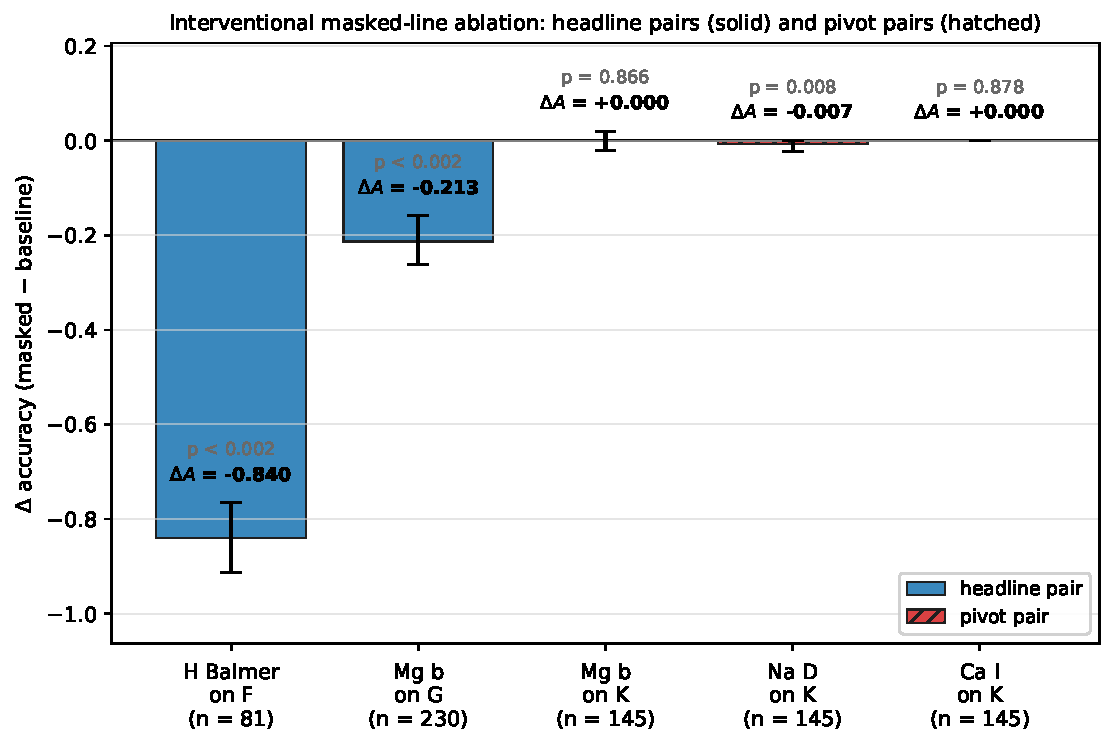
\includegraphics[width=0.85\linewidth]{ablation_bars.pdf}
\caption{Change in class recall $\dA_k^{(\mathcal{L})}$ for the headline (solid) and pivot (hatched) pairs in the primary configuration (production continuum, interpolation fill). Error bars are 95 percent bootstrap intervals (\ablNBoot{} resamples); each bar is annotated with $\dA$ and the Monte Carlo $p$-value against \ablNControls{} class-matched, bin-matched random windows (floor \ablFloor). The K bars are small but not exactly zero in rows (Section~\ref{subsec:kclass}); the values match Table~\ref{tab:ablation}.}
\label{fig:ablation}
\end{figure}

\subsection{The K class responds to no narrow window}
\label{subsec:kclass}

K-class recall barely changes under any of the five line sets (Table~\ref{tab:ablation-k}). Counting rows in the primary configuration, no line set loses more than \ablKMaxLost{} of the \nClassK{} K rows: \FeCr loses \ablPrimFeKLost{} and gains \ablPrimFeKGained{} (McNemar $p = \ablPrimFeKMcn$), (\Mgb, K) loses \ablPrimMgKLost{} and gains \ablPrimMgKGained{} ($p = \ablPrimMgKMcn$), (\NaD, K) loses \ablPrimNaKLost{} and gains \ablPrimNaKGained{} ($p = \ablPrimNaKMcn$), and (\CaI, K) loses \ablPrimCaKLost{} and gains \ablPrimCaKGained{}. The one-sided exact 95 percent upper bound on the loss rate is at most \ablKMaxUpper{} for any line set, \ablPrimMgKUpper{} for \Mgb and \NaD, and \ablPrimCaKUpper{} for \CaI. The largest decrease in K recall is \ablKMaxDrop. K recall can also rise: masking the Balmer lines gains \ablPrimHbKGained{} rows ($\dA_K = \ablPrimHbKDelta$, McNemar $p = \ablPrimHbKMcn$). This is the same temperature response as in Section~\ref{subsec:results-ablation}: a mask that makes a star look cooler can only add K rows, and the gain is not reliance of K on the masked region.

\emph{Why the Monte Carlo $p$ is not the K evidence.} For K the class-matched reference distribution is concentrated at zero: only \ablPrimNaKNullB{} of \ablNControls{} random \ablPrimNaKBins-bin windows lower K recall by as much as one row, so one lost row in (\NaD, K) ($\dA_K = \ablPrimNaKDelta$, McNemar $p = \ablPrimNaKMcn$) already gives $p_{\mathrm{MC}} = \ablPrimNaKP$. For (\FeCr, K) none of the random windows loses as many as \ablPrimFeKLost{} K rows (\ablPrimFeKNullB{} at least as extreme), so \ablPrimFeKLost{} lost rows sit at the floor, $p_{\mathrm{MC}} = \ablPrimFeKP$. These values say that the window is unusual among windows of its width, which is a statement about how rarely any window moves K, and not that the effect differs from zero. We therefore apply one standard to every K pair, namely flip counts, the exact McNemar test and the exact upper bound, and we do not call (\NaD, K) or (\FeCr, K) effects; the \FeCr result is suggestive at most.

For (\Mgb, K) the change is \ablPrimMgKDelta{} with interpolation (interval [\ablPrimMgKCiLo, \ablPrimMgKCiHi]) and \ablConstMgKDelta{} with the constant fill (\ablConstMgKLost{} lost, \ablConstMgKGained{} gained). Under polynomial\_n5 it is \ablPolyMgKDelta{} with interpolation (\ablPolyMgKLost{} lost, \ablPolyMgKGained{} gained; McNemar $p = \ablPolyMgKMcn$) and \ablPolyConstMgKDelta{} with the constant fill (\ablPolyConstMgKLost{} and \ablPolyConstMgKGained; $p = \ablPolyConstMgKMcn$). The McNemar test rejects in neither case, and the model is already degraded there. For (\CaI, K) under polynomial\_n5 the change is \ablPolyCaKDelta{} with $p_{\mathrm{MC}} = \ablPolyCaKP$. The defensible statement is that K predictions barely respond to any of the five line sets we masked (8 to 80~\AA{} total width). It is not evidence for a particular alternative route, and an upper bound is not a measurement of zero.

The \Mgb equivalent width on K spectra is not small: the median is \ewMedK~\AA{} against \ewMedG~\AA{} on G and \ewMedF~\AA{} on F (K minus G \ewDiff~\AA; KS $p = \ewKsP$). This rules out the explanation that the K \Mgb signal is too weak to matter, but \Mgb wings are a gravity indicator and the K sample is giant-dominated, so the comparison is confounded by luminosity (Section~\ref{subsec:lum}).

\begin{table}[ht]
\centering
\caption{K-class $\dA_K$ (rows lost/gained in brackets) for each line set under the 2 $\times$ 2 design: production or polynomial\_n5 continuum, each with interpolation (primary) or constant fill. The constant fill is the median of the training matrix outside the gap under the same continuum (\ablFillTrainProd{} for production, \ablFillTrainPoly{} for polynomial\_n5).}
\label{tab:ablation-k}
\small
\resizebox{\textwidth}{!}{% Generated by scripts/revision/manuscript_numbers.py from artifacts/revision/ablation_recalibrated.json
\begin{tabular}{lcccc}
\toprule
Line set & Prod., interp. & Prod., constant & Poly., interp. & Poly., constant \\
\midrule
H Balmer & \ensuremath{+0.055} (0/8) & \ensuremath{+0.028} (3/7) & \ensuremath{+0.076} (0/11) & \ensuremath{+0.076} (0/11) \\
Mg\,\textsc{b} & \ensuremath{+0.014} (1/3) & \ensuremath{0.000} (1/1) & \ensuremath{-0.014} (3/1) & \ensuremath{-0.034} (6/1) \\
Na\,\textsc{d} & \ensuremath{-0.007} (1/0) & \ensuremath{-0.007} (1/0) & \ensuremath{+0.007} (0/1) & \ensuremath{+0.007} (0/1) \\
Ca\,\textsc{i} & \ensuremath{0.000} (0/0) & \ensuremath{0.000} (0/0) & \ensuremath{-0.007} (1/0) & \ensuremath{-0.007} (1/0) \\
Fe\,\textsc{i}/Cr\,\textsc{i} & \ensuremath{-0.021} (3/0) & \ensuremath{-0.021} (3/0) & \ensuremath{-0.014} (2/0) & \ensuremath{-0.028} (4/0) \\
\bottomrule
\end{tabular}
}
\end{table}

\subsection{The luminosity-class confound}
\label{subsec:lum}

The K class is mostly giants and the F and G classes are almost all dwarfs (Table~\ref{tab:lum}, Figure~\ref{fig:kiel}). In the full sample \lumDwarfPctF{} percent of F rows, \lumDwarfPctG{} percent of G rows and \lumDwarfPctK{} percent of K rows have $\log g > \lumLoggCut$, with median $\log g$ of \lumLoggF, \lumLoggG{} and \lumLoggK. On the test set the model scores \lumAccKGiant{} on K giants ($n = \lumAccNKGiant$) and \lumAccKDwarf{} on K dwarfs ($n = \lumAccNKDwarf$); it scores \lumAccGDwarf{} on G dwarfs ($n = \lumAccNGDwarf$) and \lumAccGGiant{} on G giants ($n = \lumAccNGGiant$). The \gkErrN{} G rows predicted K include \gkErrDwarf{} dwarfs; their median $\log g$ is \gkErrLogg{} and median \Teff \gkErrTeff~K. ``K against G'' is therefore partly ``giant against dwarf''. The labels are \Teff bins on a dwarf scale, so ``K'' here means a \Teff bin that is mostly populated by red giants.

K rows also lie far from the class boundaries: the median distance to the nearest edge of the row's own \Teff bin is \bdMedK~K for K against \bdMedF{} for F and \bdMedG{} for G, and only \bdNearK{} of \nClassK{} K rows lie within \bdCut~K of an edge. Accuracy within that distance is \bdAccNearK{} for K and beyond it \bdAccFarK. Measuring the distance only to the shared 5300 and 6000~K boundaries gives a K median of \focusKMedInterior~K and \focusKNearInterior{} rows within \bdCut~K; the F and G values do not change. A push toward a hotter or cooler prediction, which is what masking a line does to a temperature estimator, rarely carries a K row across a boundary, which limits what an unchanged K recall can mean.

Table~\ref{tab:strata} splits the principal pairs by luminosity class and by boundary distance. For F and G the luminosity split is uninformative, since only three F rows and one G row are giants. Under \Mgb masking, \focusMgGDwarf{} of the \focusMgGLost{} lost G rows are dwarfs, and the loss is concentrated near the boundaries: $\dA_G = \strMgGNearDelta$ for the \strMgGNearN{} G rows within \bdCut~K of an edge of their bin against \strMgGFarDelta{} beyond it, and \focusMgGNear{} of the lost rows lie within that distance. For K, every row that changes class is a dwarf: across the five line sets \kLostDistinct{} distinct K rows are lost, \kLostDwarf{} of them dwarfs and \kLostNear{} within \bdCut~K of an edge, while K giants ($n = \lumAccNKGiant$) lose \kGiantLost{} and gain \kGiantGained{} rows. The K gains under Balmer masking are also dwarfs (\strHbKDwarfGained{} rows, $\dA_K = \strHbKDwarfDelta$ among the \strHbKDwarfN{} K dwarfs). The apparent insensitivity of the K class is therefore largely the insensitivity of its giants, which never change class under any mask.

\begin{table}[ht]
\centering
\caption{Composition and test accuracy by luminosity class. Dwarfs have $\log g > \lumLoggCut$. Fractions are over the full labelled sample; accuracies are on the held-out test rows (counts in brackets).}
\label{tab:lum}
\begin{tabular}{lrrrrcc}
\toprule
Class & $n$ & Dwarf (\%) & Median $\log g$ & Median \Teff (K) & Test acc., dwarfs & Test acc., giants \\
\midrule
F & \lumNF & \lumDwarfPctF & \lumLoggF & \lumTeffF & \lumAccFDwarf{} (\lumAccNFDwarf) & \lumAccFGiant{} (\lumAccNFGiant) \\
G & \lumNG & \lumDwarfPctG & \lumLoggG & \lumTeffG & \lumAccGDwarf{} (\lumAccNGDwarf) & \lumAccGGiant{} (\lumAccNGGiant) \\
K & \lumNK & \lumDwarfPctK & \lumLoggK & \lumTeffK & \lumAccKDwarf{} (\lumAccNKDwarf) & \lumAccKGiant{} (\lumAccNKGiant) \\
\bottomrule
\end{tabular}
\end{table}

\begin{figure}[ht]
\centering
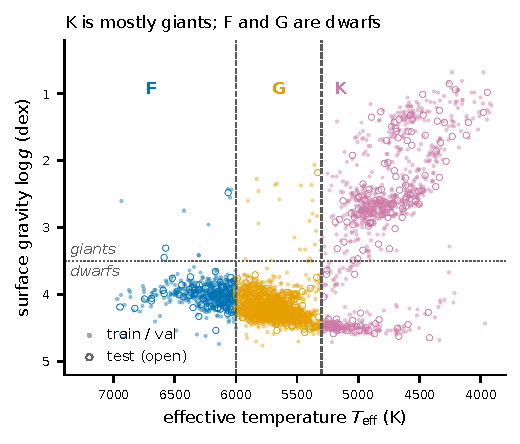
\includegraphics[width=0.8\linewidth]{kiel_diagram.pdf}
\caption{Kiel diagram of the labelled sample coloured by class. The F and G classes lie on the dwarf branch and the K class is dominated by giants; the dwarf cut is $\log g = \lumLoggCut$.}
\label{fig:kiel}
\end{figure}

\begin{table}[ht]
\centering
\caption{Ablation of the principal pairs by luminosity class and by distance to the nearest edge of the row's own \Teff bin (primary configuration). A dash marks an empty stratum.}
\label{tab:strata}
\small
\resizebox{\textwidth}{!}{% Generated by scripts/revision/manuscript_numbers.py from artifacts/revision/ablation_stratified.json
\begin{tabular}{llrrcr}
\toprule
Pair & Stratum & $n$ & $\dA$ [95\% CI] & Flips (l/g) & $\Delta\bar{P}_{\mathrm{true}}$ \\
\midrule
H Balmer, F & dwarfs & 78 & \ensuremath{-0.859} \ensuremath{[-0.936, -0.782]} & 67/0 & \ensuremath{-0.813} \\
 & giants & 3 & \ensuremath{-0.333} \ensuremath{[-1.000, +0.000]} & 1/0 & \ensuremath{-0.505} \\
 & $\leq 150$ K from boundary & 34 & \ensuremath{-0.706} \ensuremath{[-0.853, -0.559]} & 24/0 & \ensuremath{-0.667} \\
 & $> 150$ K from boundary & 47 & \ensuremath{-0.936} \ensuremath{[-1.000, -0.851]} & 44/0 & \ensuremath{-0.898} \\
\addlinespace
H Balmer, G & dwarfs & 229 & \ensuremath{-0.921} \ensuremath{[-0.952, -0.886]} & 211/0 & \ensuremath{-0.795} \\
 & giants & 1 & \ensuremath{0.000} \ensuremath{[+0.000, +0.000]} & 0/0 & \ensuremath{-0.305} \\
 & $\leq 150$ K from boundary & 72 & \ensuremath{-0.806} \ensuremath{[-0.889, -0.708]} & 58/0 & \ensuremath{-0.651} \\
 & $> 150$ K from boundary & 158 & \ensuremath{-0.968} \ensuremath{[-0.994, -0.937]} & 153/0 & \ensuremath{-0.857} \\
\addlinespace
H Balmer, K & dwarfs & 38 & \ensuremath{+0.211} \ensuremath{[+0.079, +0.342]} & 0/8 & \ensuremath{+0.181} \\
 & giants & 107 & \ensuremath{0.000} \ensuremath{[+0.000, +0.000]} & 0/0 & \ensuremath{+0.010} \\
 & $\leq 150$ K from boundary & 24 & \ensuremath{+0.292} \ensuremath{[+0.125, +0.459]} & 0/7 & \ensuremath{+0.254} \\
 & $> 150$ K from boundary & 121 & \ensuremath{+0.008} \ensuremath{[+0.000, +0.025]} & 0/1 & \ensuremath{+0.016} \\
\addlinespace
Mg\,\textsc{b}, G & dwarfs & 229 & \ensuremath{-0.258} \ensuremath{[-0.314, -0.205]} & 59/0 & \ensuremath{-0.262} \\
 & giants & 1 & \ensuremath{0.000} \ensuremath{[+0.000, +0.000]} & 0/0 & \ensuremath{0.000} \\
 & $\leq 150$ K from boundary & 72 & \ensuremath{-0.444} \ensuremath{[-0.556, -0.333]} & 32/0 & \ensuremath{-0.331} \\
 & $> 150$ K from boundary & 158 & \ensuremath{-0.171} \ensuremath{[-0.228, -0.114]} & 27/0 & \ensuremath{-0.229} \\
\addlinespace
Mg\,\textsc{b}, K & dwarfs & 38 & \ensuremath{+0.053} \ensuremath{[-0.053, +0.158]} & 1/3 & \ensuremath{+0.047} \\
 & giants & 107 & \ensuremath{0.000} \ensuremath{[+0.000, +0.000]} & 0/0 & \ensuremath{+0.004} \\
 & $\leq 150$ K from boundary & 24 & \ensuremath{+0.083} \ensuremath{[-0.083, +0.250]} & 1/3 & \ensuremath{+0.069} \\
 & $> 150$ K from boundary & 121 & \ensuremath{0.000} \ensuremath{[+0.000, +0.000]} & 0/0 & \ensuremath{+0.005} \\
\addlinespace
Na\,\textsc{d}, K & dwarfs & 38 & \ensuremath{-0.026} \ensuremath{[-0.079, +0.000]} & 1/0 & \ensuremath{-0.010} \\
 & giants & 107 & \ensuremath{0.000} \ensuremath{[+0.000, +0.000]} & 0/0 & \ensuremath{-0.001} \\
 & $\leq 150$ K from boundary & 24 & \ensuremath{-0.042} \ensuremath{[-0.125, +0.000]} & 1/0 & \ensuremath{-0.015} \\
 & $> 150$ K from boundary & 121 & \ensuremath{0.000} \ensuremath{[+0.000, +0.000]} & 0/0 & \ensuremath{-0.001} \\
\addlinespace
Ca\,\textsc{i}, K & dwarfs & 38 & \ensuremath{0.000} \ensuremath{[+0.000, +0.000]} & 0/0 & \ensuremath{-0.001} \\
 & giants & 107 & \ensuremath{0.000} \ensuremath{[+0.000, +0.000]} & 0/0 & \ensuremath{0.000} \\
 & $\leq 150$ K from boundary & 24 & \ensuremath{0.000} \ensuremath{[+0.000, +0.000]} & 0/0 & \ensuremath{-0.001} \\
 & $> 150$ K from boundary & 121 & \ensuremath{0.000} \ensuremath{[+0.000, +0.000]} & 0/0 & \ensuremath{0.000} \\
\addlinespace
Fe\,\textsc{i}/Cr\,\textsc{i}, K & dwarfs & 38 & \ensuremath{-0.079} \ensuremath{[-0.184, +0.000]} & 3/0 & \ensuremath{-0.049} \\
 & giants & 107 & \ensuremath{0.000} \ensuremath{[+0.000, +0.000]} & 0/0 & \ensuremath{-0.005} \\
 & $\leq 150$ K from boundary & 24 & \ensuremath{-0.083} \ensuremath{[-0.208, +0.000]} & 2/0 & \ensuremath{-0.051} \\
 & $> 150$ K from boundary & 121 & \ensuremath{-0.008} \ensuremath{[-0.025, +0.000]} & 1/0 & \ensuremath{-0.009} \\
\bottomrule
\end{tabular}
}
\end{table}

\subsection{Scale mismatch under polynomial re-normalisation}
\label{subsec:scale}

Re-deriving the continuum of the test rows with a sigma-clipped polynomial lowers G recall from \sdProdRecG{} to \sdPolyRecG{} and macro-F1 from \sdProdMacroF{} to \sdPolyMacroF, with \sdGtoKPoly{} of \nClassG{} G rows moving to K and \sdPolyGtoF{} to F (Table~\ref{tab:scale}). The re-normalisation changes two things at once: it removes the class-dependent level spread, and it lifts the global median level from \sdMedProdGlobal{} to \sdMedPolyGlobal, about \sdPolyShiftPct{} percent. Gradient-boosted trees split on absolute thresholds, so a level shift can move every bin across a split. The decomposition with the model held fixed separates the two effects (Table~\ref{tab:scale}, Figure~\ref{fig:continuum_medians}).

\begin{itemize}
\item Removing the spread while keeping the scale (every row rescaled to the common test median) costs \sdCostCommon{} in macro-F1 (to \sdCommonMacroF) and leaves \sdCommonGtoK{} G rows going to K.
\item Keeping the spread and shifting the scale (every row multiplied by \sdUniMult) reproduces the collapse: macro-F1 \sdUniNineMacroF, G recall \sdUniNineRecG, and \sdUniNineGtoK{} G rows going to K. The ratio of the global medians, \sdBestMult, gives \sdUniBestMacroF{} and \sdUniBestGtoK{} rows.
\item Swapping the G and K median levels costs \sdCostSwap{} and raises G$\to$K to \sdSwapGtoK.
\item Restoring the production values of the gap bins after re-normalisation changes macro-F1 by less than 0.005 (\sdPolyGapMacroF{} against \sdPolyMacroF), so the gap bins do not carry the effect.
\end{itemize}
The level itself holds weak class information. A one-feature logistic regression on the per-row off-gap median reaches accuracy \oneAcc{} (balanced accuracy \oneBal) on the test set, with ROC AUC \oneAucGK{} for G against K and \oneAucFG{} for F against G. The per-class median of the row medians is \medProdF{} (F), \medProdG{} (G) and \medProdK{} (K) under the production normalisation, a spread of \spreadProd{} percentage points with KS $p$ of \ksProdFG{} (F--G), \ksProdGK{} (G--K) and \ksProdFK{} (F--K). After the polynomial fit the medians are \medPolyF, \medPolyG{} and \medPolyK{} (a spread of \spreadPoly{} points, with the order reversed), and the KS $p$ are \ksPolyFG, \ksPolyGK{} and \ksPolyFK. The level carries real but weak class information, but a model that read only the level could not reach G recall of \sdProdRecG, and after re-normalisation all three class medians lie above the production F median, so a model that read the level would be expected to move G toward F rather than K. We conclude that the polynomial collapse is a train--test scale mismatch: the model has not seen the scale of the re-normalised inputs. This is brittleness to a normalisation convention, which is a failure to transfer to a shifted condition. We do not identify a specific unintended feature the model relies on, and we therefore do not call it shortcut learning.

\begin{table}[ht]
\centering
\caption{The fixed production model scored on transformed test spectra. Recall per class, macro-F1 and the number of G rows predicted K, with the median row level in the last column. ``Spread removed'' rescales each row to the common test median; ``G/K swap'' exchanges the two class median levels.}
\label{tab:scale}
\small
\begin{tabular}{lrrrrrr}
\toprule
Transformation & $R_F$ & $R_G$ & $R_K$ & macro-F1 & G$\to$K & Median level \\
\midrule
Production & \sdProdRecF & \sdProdRecG & \sdProdRecK & \sdProdMacroF & \sdProdGtoK & \sdProdLevel \\
Polynomial\_n5 & \sdPolyRecF & \sdPolyRecG & \sdPolyRecK & \sdPolyMacroF & \sdPolyGtoK & \sdPolyLevel \\
Polynomial\_n5, gap restored & \sdPolyGapRecF & \sdPolyGapRecG & \sdPolyGapRecK & \sdPolyGapMacroF & \sdPolyGapGtoK & \sdPolyGapLevel \\
Spread removed, scale kept & \sdCommonRecF & \sdCommonRecG & \sdCommonRecK & \sdCommonMacroF & \sdCommonGtoK & \sdCommonLevel \\
Every row $\times$ \sdUniMult & \sdUniNineRecF & \sdUniNineRecG & \sdUniNineRecK & \sdUniNineMacroF & \sdUniNineGtoK & \sdUniNineLevel \\
Every row $\times$ \sdBestMult & \sdUniBestRecF & \sdUniBestRecG & \sdUniBestRecK & \sdUniBestMacroF & \sdUniBestGtoK & \sdUniBestLevel \\
G/K swap & \sdSwapRecF & \sdSwapRecG & \sdSwapRecK & \sdSwapMacroF & \sdSwapGtoK & \sdSwapLevel \\
\bottomrule
\end{tabular}
\end{table}

\begin{figure}[ht]
\centering
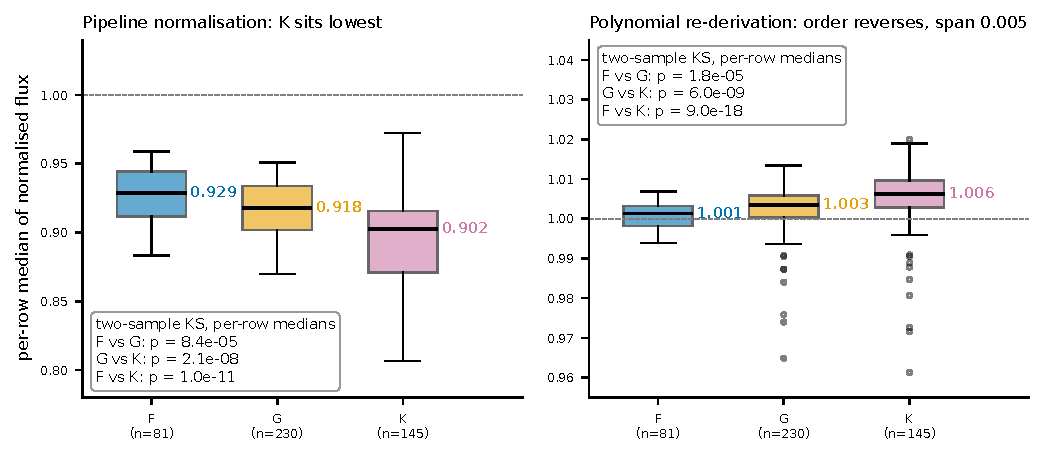
\includegraphics[width=0.92\linewidth]{continuum_medians.pdf}
\caption{Per-row median of normalised flux outside the inter-chip gap by class on the test set, under the production normalisation (left) and after the polynomial re-normalisation (right). Class medians are given in Section~\ref{subsec:scale}; the numbers come from the same artifact as Table~\ref{tab:scale}.}
\label{fig:continuum_medians}
\end{figure}

\subsection{Retraining on re-normalised spectra}
\label{subsec:retrain}

We ran the retraining experiment that tests whether the K result depends on the continuum convention (Table~\ref{tab:retrain}). The production retrain reproduces the deposited model exactly (macro-F1 difference \rtReproDiff, identical confusion matrix, best iteration \rtProdIter). Retrained on polynomial\_n5 features the model reaches macro-F1 \rtPolyMacroF{} and on row-median-normalised features \rtRowMedMacroF, a loss of \rtDeltaMacroPoly{} and \rtDeltaMacroRow{} against the production \rtProdMacroF. This is within the fold-to-fold spread of 5-fold cross-validation on the production matrix (\rtCvMean{} with sample SD \rtCvSd). The classifier loses about a hundredth of macro-F1 without the level, so the level is not what carries performance. In every retrained model the (\Mgb, K) change is null or slightly positive (\rtProdMgKDelta, \rtPolyMgKDelta, \rtPolyGapMgKDelta, \rtRowMedMgKDelta{} for the four matrices), while (\Mgb, G) is clearly negative (\rtProdMgGDelta, \rtPolyMgGDelta, \rtPolyGapMgGDelta, \rtRowMedMgGDelta). The change in K recall seen when the fixed model scores polynomial-normalised inputs (\ablPolyMgKDelta{} with interpolation and \ablPolyConstMgKDelta{} with the constant fill; Table~\ref{tab:ablation-k}) is therefore a response of a model scored far from its training conditions (baseline accuracy \ablBaseAccPoly), not a property of the K class. The retraining was first planned as future work; because the same rows train, validate and test, it does not invalidate the split. The \Mgb results do not depend on the normalisation convention.

\begin{table}[ht]
\centering
\caption{LightGBM retrained with the production hyperparameters on each feature matrix (same train/validation/test rows). Recall per class, macro-F1, G rows predicted K, and the \Mgb ablation on K and G (constant fill at the test-matrix median, class-matched null, \rtNControls{} windows, \rtNBoot{} bootstrap resamples). Intervals are 95 percent bootstrap intervals.}
\label{tab:retrain}
\footnotesize
\resizebox{\textwidth}{!}{%
\begin{tabular}{lrrrrrcc}
\toprule
Features & $R_F$ & $R_G$ & $R_K$ & macro-F1 & G$\to$K & $\dA_K$ (\Mgb) [95\%] ($p_{\mathrm{MC}}$) & $\dA_G$ (\Mgb) [95\%] ($p_{\mathrm{MC}}$) \\
\midrule
Production & \rtProdRecF & \rtProdRecG & \rtProdRecK & \rtProdMacroF & \rtProdGtoK & \rtProdMgKDelta{} [\rtProdMgKCiLo, \rtProdMgKCiHi] (\rtProdMgKP) & \rtProdMgGDelta{} [\rtProdMgGCiLo, \rtProdMgGCiHi] (\rtProdMgGP) \\
Polynomial\_n5 & \rtPolyRecF & \rtPolyRecG & \rtPolyRecK & \rtPolyMacroF & \rtPolyGtoK & \rtPolyMgKDelta{} [\rtPolyMgKCiLo, \rtPolyMgKCiHi] (\rtPolyMgKP) & \rtPolyMgGDelta{} [\rtPolyMgGCiLo, \rtPolyMgGCiHi] (\rtPolyMgGP) \\
Polynomial\_n5, gap restored & \rtPolyGapRecF & \rtPolyGapRecG & \rtPolyGapRecK & \rtPolyGapMacroF & \rtPolyGapGtoK & \rtPolyGapMgKDelta{} [\rtPolyGapMgKCiLo, \rtPolyGapMgKCiHi] (\rtPolyGapMgKP) & \rtPolyGapMgGDelta{} [\rtPolyGapMgGCiLo, \rtPolyGapMgGCiHi] (\rtPolyGapMgGP) \\
Row-median & \rtRowMedRecF & \rtRowMedRecG & \rtRowMedRecK & \rtRowMedMacroF & \rtRowMedGtoK & \rtRowMedMgKDelta{} [\rtRowMedMgKCiLo, \rtRowMedMgKCiHi] (\rtRowMedMgKP) & \rtRowMedMgGDelta{} [\rtRowMedMgGCiLo, \rtRowMedMgGCiHi] (\rtRowMedMgGP) \\
\bottomrule
\end{tabular}}
\end{table}

\subsection{Robustness of the (\texorpdfstring{\Mgb}{Mg b}, K) effect to training choices}
\label{subsec:robustness}

Two further retrains were run on the production features with the deposited constant fill. With uniform class weights the model reaches macro-F1 \uwMacroF{} and the (\Mgb, K) change is \uwDelta. Across a $3 \times 3$ grid of \texttt{max\_depth} $\in \{6, 8, 10\}$ and \texttt{num\_leaves} $\in \{31, 63, 127\}$ (\gridNCells{} cells) the largest absolute change is \gridMaxDelta. The grid does not vary the learning rate, the column subsampling, the objective or the regularisation, so this is a statement about those nine cells and not about gradient-boosted trees in general.

\section{Discussion}
\label{sec:discussion}

\paragraph{What the audit adds.} A fixed, pre-specified list of line sets, a per-class readout and a class-matched, bin-matched null make the answer to ``does this classifier depend on this window for this class'' reproducible, and the flip counts and McNemar test make the K-class statement honest about how few rows move. The method is an operation on the input domain of a fixed model and does not depend on the architecture. It does not separate a physical dependence from a response to an edited input, since masking and interpolation can leave the data manifold \citep{Hooker2019Benchmark,Covert2021Removing}, and it measures reliance on a window, not the causal effect of a stellar property. The prior-art approaches that build the dependence structure into the model \citep{2019ApJ...879...69T,2019ApJS..245...34X,2019MNRAS.483.3255L} answer a different question: how to constrain a model, where we probe an unconstrained one.

\paragraph{Attribution baselines and ablation.} The three baselines of Section~\ref{subsec:triangulation} point at the Balmer and \Mgb regions and disagree elsewhere. A ranking says where the model looks; only the intervention says whether the prediction changes when the region is edited, and K-class insensitivity is a property of that response. The scale mismatch is not an attribution result at all: it appears when the per-class level and the global scale of the inputs are examined directly.

\paragraph{The scale mismatch.} The earlier reading, that the model used the per-class continuum level as its main G-versus-K discriminator, fails three tests. A uniform rescaling that keeps the spread reproduces the collapse; removing the spread while keeping the scale does not; and retraining without the level costs about a hundredth of macro-F1. For pipeline-normalised spectra the practical lesson is that a tree model scored on a re-normalised matrix, even by a small uniform shift, should be treated as scored on shifted inputs. We recommend reporting the normalisation convention, the global median level, and a uniform-rescaling sensitivity check alongside any such evaluation.

\paragraph{What the K result does and does not say.} K recall does not respond to any narrow window: K giants, which are \lumAccNKGiant{} of the \nClassK{} K test rows, lose \kGiantLost{} and gain \kGiantGained{} rows under all five masks. The class is giant-dominated, sits far from the class edges, and has many redundant temperature-sensitive features, so a narrow mask removes little that other bins cannot supply. We do not infer a shortcut from that, and the \FeCr result is suggestive at most. Comparing with an external parameter-inference network such as that of \citet{2024A&A...692A.228C} is not informative here, since it is a different task on a different instrument.

\section{Limitations}
\label{sec:limitations}

\textbf{Labels and luminosity.} The classes are \Teff bins from parameters derived from the same spectra, on a dwarf scale, and the K class is giant-dominated. The audit tests reproduction of a spectroscopic \Teff bin, and no claim about MK classification in the full spectral and luminosity sense follows. Restricting the audit to dwarfs would leave only \lumNDwarfKtest{} K test rows.

\textbf{Resolution and blends.} The bins correspond to $R \approx 2000$, so a line window is a blend (Table~\ref{tab:linesets}) and the native UVES resolving power is not used by the features. The \Mgb window contains \FeI lines, and ``\Mgb dependence'' means dependence on that 21~\AA{} region. The window widths differ by a factor of about ten, from 8 to 80~\AA, which is why the nulls are matched in bin count and drawn per class.

\textbf{Interventions.} Interpolation and constant fills are off-distribution edits. The ablation is on a single model, one instrument and one survey, with the GES parameters as labels. Effects based on a few rows do not support claims beyond the sample. The indifference zone was chosen after the data were seen and is descriptive.

\textbf{Leakage and spatial structure.} Because \singRowPct{} percent of train+val rows are in singleton spatial groups, the spatial pass does not bound cluster leakage tightly, and a residual contribution of order one to two points of macro-F1 cannot be excluded. The spatial group identifiers are re-derived, not deposited.

\textbf{External check.} The template cross-check failed its gate and so offers no corroboration (Appendix~\ref{app:pickles}).

\section{Conclusions}
\label{sec:conclusions}

A LightGBM classifier of three \Teff-bin classes on Gaia-ESO UVES U580 spectra reaches macro-F1 \testMacroF. Under pre-specified masked-line ablation, the F class depends on the Balmer region and the G class on the \Mgb region: masking them changes recall by \ablPrimHbFDelta{} and \ablPrimMgGDelta{} (\ablPrimHbFLost{} and \ablPrimMgGLost{} rows lost, \ablPrimMgGGained{} gained for \Mgb), and rows move as a temperature estimator would move them. The size of the Balmer effect and the destination of its errors depend on the fill; the \Mgb effect does not (\ablConstMgGDelta{} with the constant fill). The K class does not respond to any narrow window we tried: no line set loses more than \ablKMaxLost{} of \nClassK{} K rows, and masks that make a star look cooler add K rows. That is the full content of the K result. Its evidence is flip counts, exact McNemar tests and upper bounds, since the Monte Carlo $p$-values are near-degenerate for K, and it is a failure to detect a dependence in a giant-dominated class, not a finding about what the K class reads instead. The earlier claim of a class-level continuum shortcut does not survive: the collapse under polynomial re-normalisation is a train--test scale mismatch that a uniform \sdUniMult{} rescaling reproduces, and retraining on re-normalised spectra restores the classifier and leaves the \Mgb effect on K null. For anyone scoring a tree model on re-normalised spectra the caution is practical: report the normalisation convention and the global level, and check sensitivity to a uniform rescaling. The code, model, feature matrix, decision log and every number-producing script are released so that the same probe can be run on other classifiers.

\section*{Data and code availability}

Code is available at \url{https://github.com/TirtheshJani/ges-uves-mk-audit} under the MIT licence. The trained model (\texttt{lgbm\_mk.pkl}), the feature matrix (\texttt{features.npz}) and the numerical artifacts are deposited at Zenodo (DOI: to be assigned on Zenodo deposit) with the same release tag as the GitHub repository. Reproduction commands, seeds and run times are in \texttt{docs/reproducibility\_appendix.md}; the provenance of the three local copies of the project is in \texttt{docs/folder\_provenance.md} and the dated decision log is \texttt{docs/decision\_log.md}. Every number in this paper is written to \texttt{submission/revision\_numbers.tex} by \texttt{scripts/revision/manuscript\_numbers.py}, and \texttt{artifacts/revision/manuscript\_numbers\_index.json} maps each macro to its source artifact. The Gaia-ESO data are public through the ESO Science Archive Facility. The Pickles library is public through the STScI HLSP reference-atlases mirror and is not redistributed.

\section*{Acknowledgements}

This work uses data from the Gaia-ESO Public Spectroscopic Survey, ESO programme 188.B-3002, conducted with the FLAMES instrument at the VLT \citep{2022A&A...666A.120G,2014A&A...565A.113S}. Stellar parameters used for the labels are from \citet{2023A&A...676A.129H}. Atomic line rest wavelengths are from the NIST Atomic Spectra Database \citep{NIST_ASD_2023}. The Pickles library was retrieved from the STScI HLSP reference-atlases mirror. Software includes LightGBM \citep{Ke2017LightGBM}, SHAP \citep{LundbergLee2017SHAP,Lundberg2020TreeSHAP}, scikit-learn, numpy, scipy, astropy, astroquery and matplotlib.

\bibliographystyle{plainnat}
\bibliography{manuscript_citations}

\appendix

\section{External cross-check against the Pickles library: not passed}
\label{app:pickles}

\noindent\emph{No continuum convention reached the pre-specified agreement gate. The cross-check is reported as a failed external check, not as corroboration.}

We compared each test spectrum with the \pkNTemplates{} spectra of the Pickles UVKLIB library \citep{1998PASP..110..863P} by minimising a unit-variance chi-squared over bins finite in both spectra, and compared the spectral type of the best template with the classifier's prediction. The spectral type of each template is read from the \texttt{COMMENT1} card of its FITS header; the earlier version of this check used a hand-built index map that was mis-assigned from index 17 onward because the library interleaves metal-weak and metal-rich variants, and that map and its results are withdrawn. The embedded map now agrees with the headers for \pkEmbedAgree{} of \pkNTemplates{} templates, and the distribution assigns types in luminosity order (V, IV, III, II, I). The agreement gate was \pkGate{} with at least \pkGateMinN{} compared rows.

Table~\ref{tab:pickles} gives the result. The best agreement, \pkAgreeMfTwo{} for the 200~\AA{} median-filter normalisation, is below the gate. For that normalisation \pkSuperMfTwo{} percent of best-matching templates are supergiants, so the comparison is dominated by a luminosity class that is essentially absent from the test sample, and the agreement says little about the classifier. The polynomial\_n5 convention yields no F, G or K template matches (all rows land on templates outside the class range), and the additional variant fitted on the 4700 to 6900~\AA{} window only reaches \pkAgreePolyWin. A template library without luminosity or metallicity matching to the sample cannot test a three-class \Teff classifier at this resolution, and we have not tried to repair it. We cut the earlier confusion-matrix figure, which was produced with the withdrawn map.

\begin{table}[ht]
\centering
\caption{Agreement between the classifier and the spectral type of the best-matching Pickles template under four continuum conventions (gate: agreement $\ge \pkGate$ and at least \pkGateMinN{} compared rows). ``Super.'' is the fraction of best-matching templates that are supergiants. The polynomial\_n5 convention gives no F, G or K matches. The last row is an additional variant fitted on a restricted window and is not part of the pre-specified set.}
\label{tab:pickles}
\begin{tabular}{lrrrr}
\toprule
Convention & $n_{\mathrm{FGK}}$ & Agreement & Macro-F1 & Super. (\%) \\
\midrule
200~\AA{} median filter & \pkNMfTwo & \pkAgreeMfTwo & \pkMacroMfTwo & \pkSuperMfTwo \\
50~\AA{} median filter & \pkNMfFifty & \pkAgreeMfFifty & \pkMacroMfFifty & \pkSuperMfFifty \\
Polynomial $n=5$ (sigma-clipped) & \pkNPolyN & \pkAgreePolyN & \pkMacroPolyN & \pkSuperPolyN \\
Polynomial $n=5$, 4700--6900~\AA{} window & \pkNPolyWin & \pkAgreePolyWin & \pkMacroPolyWin & \pkSuperPolyWin \\
\bottomrule
\end{tabular}
\end{table}

\section{Attribution and confusion figures}

\begin{figure}[ht]
\centering
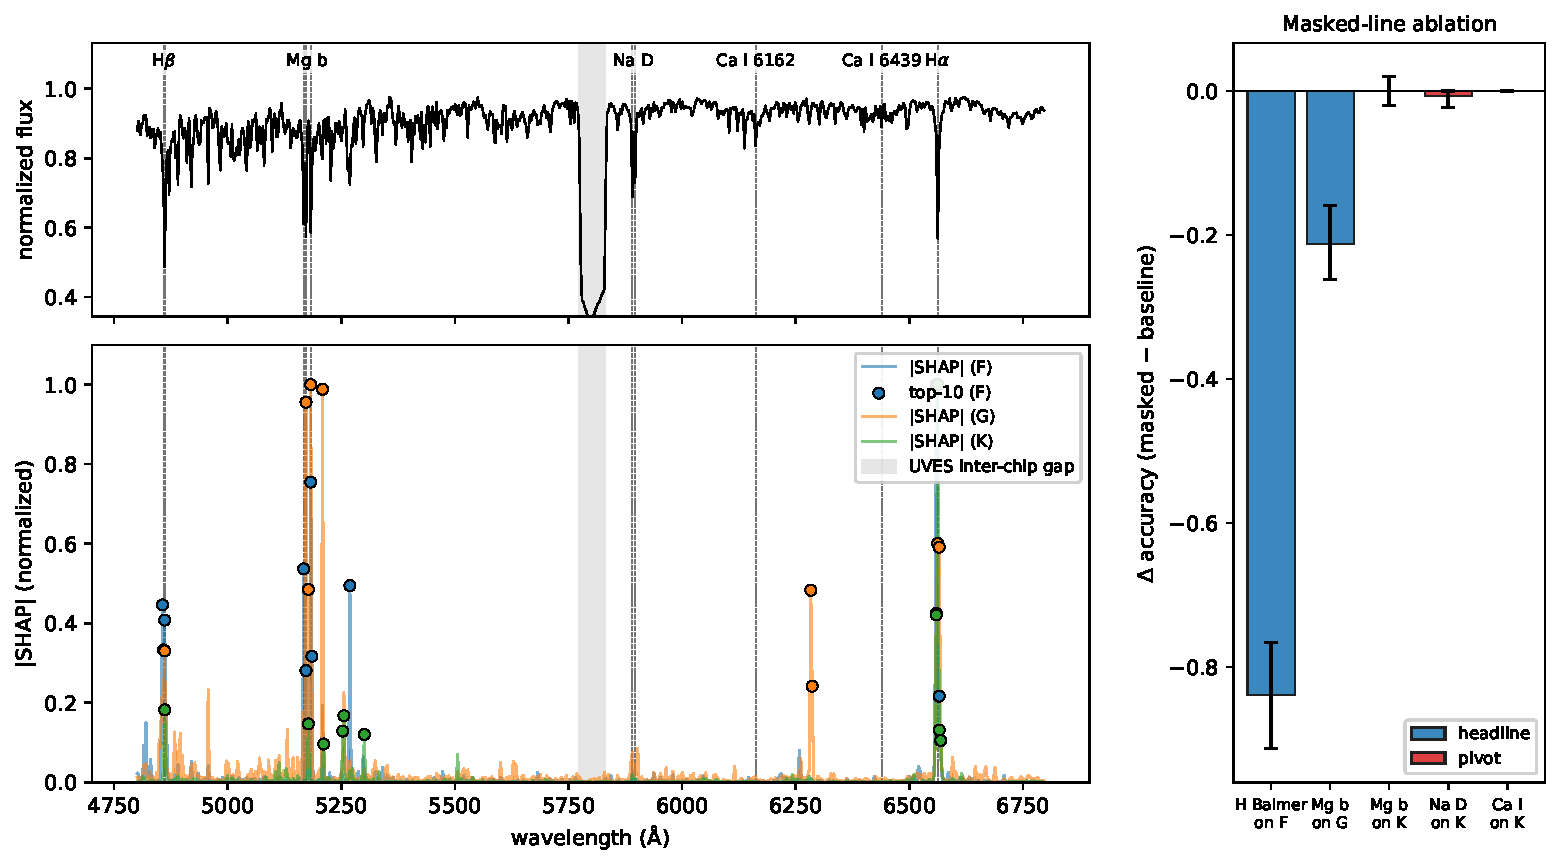
\includegraphics[width=0.92\linewidth]{importance_main.pdf}
\caption{Top: per-bin median normalised spectrum of the G class with the diagnostic-line positions marked and the inter-chip gap shaded. Bottom: normalised mean $|\mathrm{SHAP}|$ per class (F blue, G orange, K green) with the ten largest bins of each class marked. Right: $\dA$ (change in per-class accuracy, that is recall) for the headline and pivot pairs from the primary ablation run (production continuum, linear-interpolation fill), with 95 percent bootstrap intervals; the same quantities with their random-window $p$-values are in Figure~\ref{fig:ablation} and Table~\ref{tab:ablation}.}
\label{fig:importance}
\end{figure}

\begin{figure}[ht]
\centering
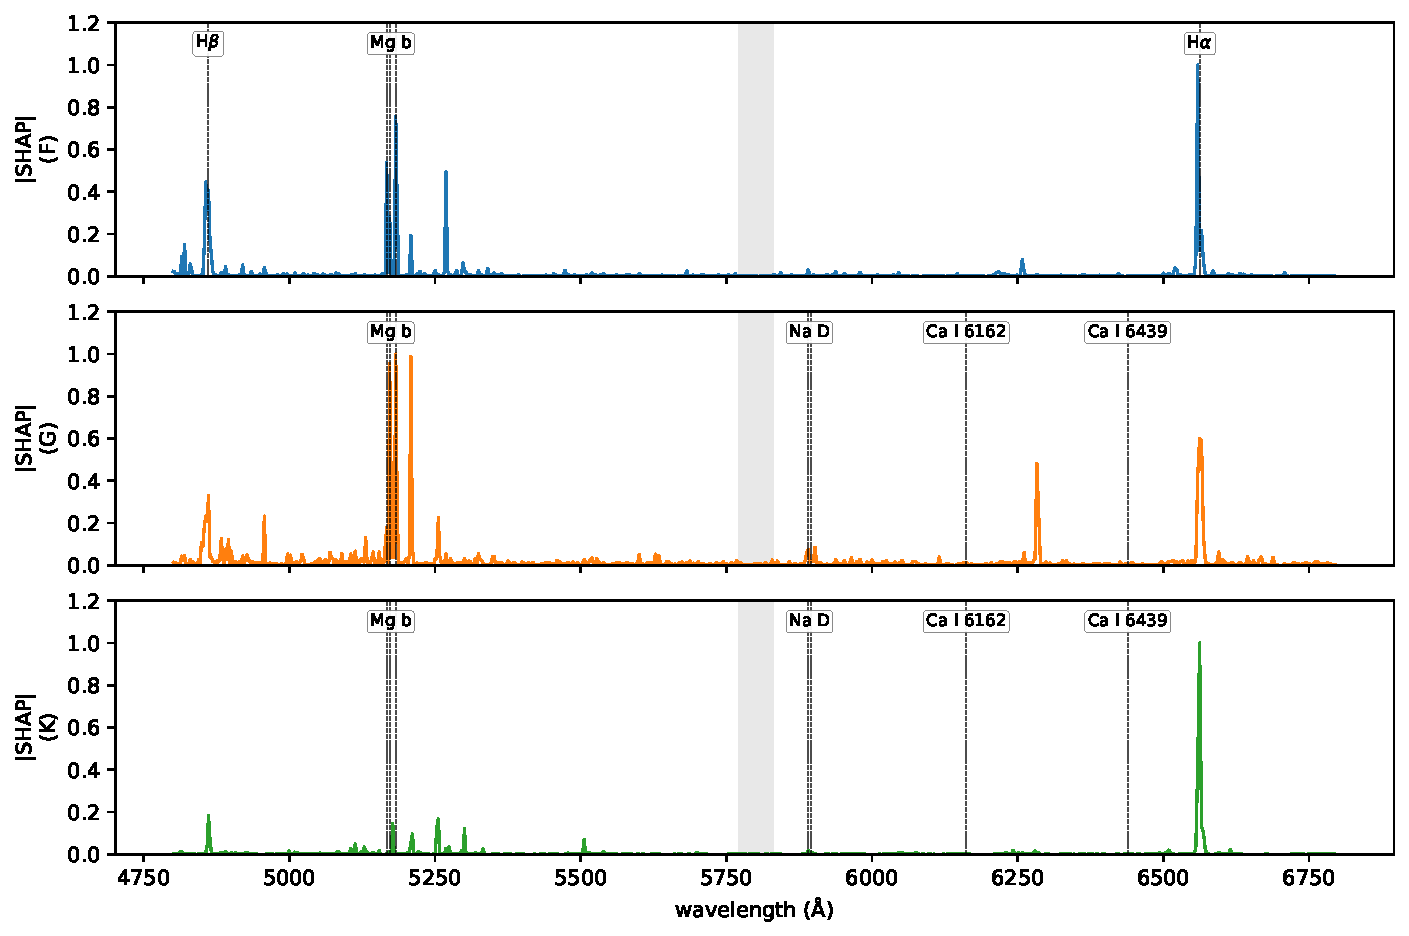
\includegraphics[width=0.82\linewidth]{importance_per_class_gapmask.pdf}
\caption{Per-class SHAP overlay with the inter-chip gap shaded.}
\label{fig:perclass}
\end{figure}

\begin{figure}[ht]
\centering
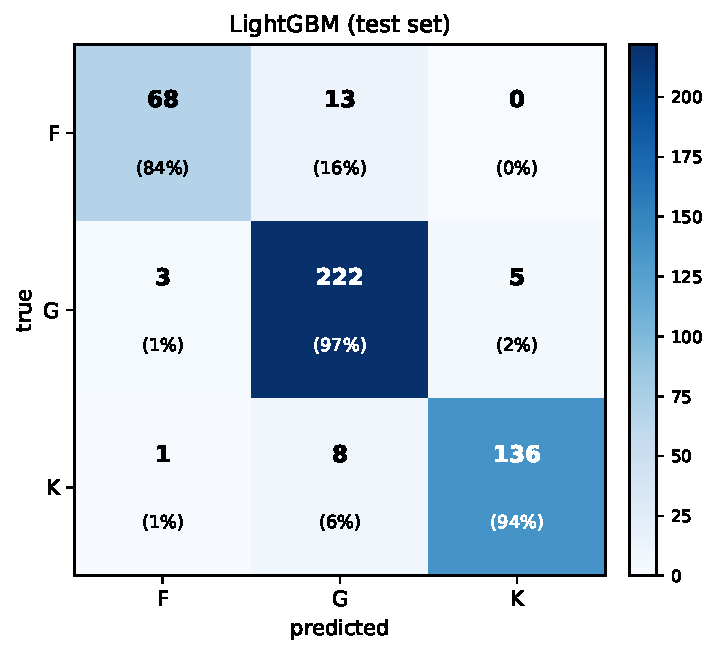
\includegraphics[width=0.55\linewidth]{confusion_matrix_test.pdf}
\caption{Held-out test confusion matrix. Rows are the true class and columns the predicted class, in F--G--K order.}
\label{fig:confusion}
\end{figure}

\end{document}
